% AU template last modified by AU: 2010 Jul 02
% SH modifications for Markdown made in September 2018

\documentclass[12pt,econ]{sources/authesis}
\usepackage{natbib}  % natbib citation style
% The following packages are for the LaTeX generated graph
\usepackage{threeparttable}
\usepackage{tikz}
\usetikzlibrary{arrows}
\usepackage{tikz}
\usepackage{lscape}
\usepackage[hidelinks]{hyperref}
\usepackage{float} % to float tables
\usepackage{longtable} % for tables that are longer than one page
\usepackage{booktabs} % for stuff like \bottomrule in tables
\usepackage{adjustbox} % for \resizebox for tables
\usepackage{dcolumn} % to align on the decimal point of numbers in table columns
\usepackage{bm} % to make math symbols bold with \bm{}
\usepackage{changepage} % for \adjustwidth
\usepackage{amsfonts} % for math symbol "mathfrak"

% next 11 lines to create math symbol "reallywidehat"
\usepackage{scalerel,stackengine}
\stackMath
\newcommand\reallywidehat[1]{%
\savestack{\tmpbox}{\stretchto{%
  \scaleto{%
    \scalerel*[\widthof{\ensuremath{#1}}]{\kern-.6pt\bigwedge\kern-.6pt}%
    {\rule[-\textheight/2]{1ex}{\textheight}}%WIDTH-LIMITED BIG WEDGE
  }{\textheight}% 
}{0.5ex}}%
\stackon[1pt]{#1}{\tmpbox}%
}


%%-------------------------------------------------
%% For flowchart(s)
%%-------------------------------------------------

\usepackage{tikz}
\usetikzlibrary{shapes,arrows,positioning}

% Define block
\tikzstyle{block} = [rectangle, draw, fill=blue!20, text width=1cm, text centered, rounded corners, minimum height=3em]

% Define another block
\tikzstyle{block2} = [rectangle, draw, fill=blue!20, text width=3cm, text centered, rounded corners, minimum height=2em]

% Define another block
\tikzstyle{block2r} = [rectangle, draw, fill=red!20, text width=3cm, text centered, rounded corners, minimum height=2em]

% Define yet another block
\tikzstyle{block3} = [rectangle, draw, fill=blue!20, text width=2cm, text centered, rounded corners, minimum height=3em]

% And another block
\tikzstyle{block4} = [rectangle, draw, text width=3cm, text centered, rounded corners, minimum height=3em]

% Define cloud
\tikzstyle{cloud} = [draw, ellipse, fill=red!20, node distance=1cm, minimum height=3em]

% Define another cloud
\tikzstyle{cloud2} = [draw, ellipse, node distance=1cm, minimum height=3em]

% Define another cloud
\tikzstyle{cloud3} = [draw, ellipse, fill=red!20, node distance=1cm, minimum height=2em]

% Define line
\tikzstyle{line} = [draw, -latex', node distance = 0.1cm, auto]


% 
% FIGURES
%
\usepackage{graphicx}
% SH: The following generates all images so they have a width \maxwidth. This means that they will get their normal width if they fit onto the page, but are scaled down if they would overflow the margins:
\makeatletter
\def\maxwidth{\ifdim\Gin@nat@width>\linewidth\linewidth
\else\Gin@nat@width\fi}
\makeatother
\let\Oldincludegraphics\includegraphics
\renewcommand{\includegraphics}[1]{\Oldincludegraphics[width=\maxwidth]{#1}}
% SH: The following is repeated from the .cls file to make it appear in Markdown. The commands set the figure float, count etc.
\makeatletter
\def\fps@figure{ht} 
\def\ftype@figure{1}
\def\ext@figure{lof}
\def\fnum@figure{\figurename~\thefigure}
\def\figure{\@float{figure}}
\let\endfigure\end@float
\@namedef{figure*}{\@dblfloat{figure}}
\@namedef{endfigure*}{\end@dblfloat}
\makeatother
% SH: The following is repeated from the .cls file to make it appear in Markdown. The commands set the captions and also make the lof and lot double-spaced (unless it extends to more than one line, in which case it's single-spaced)
\makeatletter
\def\caption{\refstepcounter\@captype \@dblarg{\@caption\@captype}}
\long\def\@caption#1[#2]#3{%
  \par \par
  \addcontentsline{\csname ext@#1\endcsname}{#1}%
    {\protect\numberline{\csname the#1\endcsname.}{\ignorespaces #2}}%
  \addtocontents{\csname ext@#1\endcsname}{\protect\addvspace{10\p@}}%
  \begingroup
    \@parboxrestore
    \if@minipage
      \@setminipage
    \fi
    \normalsize
    \itshape % SH: Added \itshape myself for aesthetics -- to distinguish figure caps from text
    \@makecaption{\csname fnum@#1\endcsname}{\ignorespaces #3}\par
  \endgroup}
\makeatother
% end SH



% Declarations for Front Matter
%
% IMPORTANT: IF A TITLE OR SUBTITLE EXCEEDS MORE THAN ONE LINE,
%            THERE SHOULD ONLY BE  48 CHARACTERS PER LINE.
%
% The dissertation title must be capitalized for AU-CAS

\title{WHAT THE PEOPLE THINK: ADVANCES IN PUBLIC OPINION MEASUREMENT USING ORDINAL VARIABLES}
\author{Simon Heuberger}
\degreeyear{2020}
\degree{Doctor of Philosophy}
\chair{Professor Jeff Gill}
\secondreader{Professor Ryan T. Moore}
\thirdreader{Professor Elizabeth Suhay}
\fourthreader{Professor R. Michael Alvarez}
\degreefield{Government}

\begin{document}

\maketitle

\maketitle

% The following command makes the copyright page

\copyrightpage

% The frontmatter environment uses roman lower case page numbering. The
% abstract, acknowledgements, table of contents, list of figures, and
% list of tables are a part of this environment.
\begin{frontmatter}

% The Guide requires one numbered abstract page.
% The 'abstractn' macro generates a numbered abstract page.
% Do NOT use the 'abstract' macro, which generates an unnumbered, abstract page.
% (NOTE: The Guide no longer requires two abstract pages, one numbered, one without numbers.)

\abstractn{Surveys are a central part of political science. Without surveys, we would not know what people think about political issues. Survey experiments further enable us to test how people react to given treatments. Surveys and survey experiments are only as good as the measurements and analytical techniques we as researchers employ, though. For one particular survey variable called ordinal variables, some of our current measurements and techniques are insufficient. Ordinal variables consist of ordered categories where the spacing between each category is uneven and not known. Ordinal variables are highly important because the most important predictor of political behavior is an ordinal variable: Education. Ordinal example categories for education could be ``Some High School'', ``High School Graduate'', and ``Bachelor's Degree''. The literature currently often does not take the special nature of ordinal variables, i.e.~their uneven spacing, into account. This could misrepresent the data and potentially distort survey results. It is important that we measure and use education and other ordinal variables correctly. My dissertation develops two methods to do so and applies them in original survey research. Chapter II develops a new method to improve the use of ordinal variables in the assignment of treatment in survey experiments. Chapter III develops a new method to treat missing survey data with ordinal variables. Chapter IV applies both methods in an online survey experiment on political framing.}

%This is an abstractn.  There are page numbers.
%The \emph{Guide} says an abstract should not exceed 350 words.
%(If you do exceed this,
%then under the CAS option, the first page is numbered bottom center, and %the rest are numbered top right.)


% Acknowledgements are optional. If you do not wish to include them,
% simply do not include this command in your source.

\acknowledgements{I want to thank Fendi and Muesli, the two greatest creatures on the planet. And of course Waldemar Burgo.}


\listoftables

\listoffigures

\tableofcontents


\end{frontmatter}

\hypertarget{intro}{%
\chapter{INTRODUCTION}\label{intro}}

\hypertarget{intro-ordinal}{%
\section{Ordinal Variables}\label{intro-ordinal}}

Ordinal variables matter in surveys. One of the most important ordinal variables in political science surveys is education. It is widely established that education represents one of the major driving forces behind public opinion and political behavior, such as turnout or donations, in the U.S. (Abramowitz, 2010; Dawood, 2015; Druckman, Peterson, \& Slothuus, 2013; Fiorina \& Abrams, 2009; Fiorina, Abrams, \& Pope, 2011; King, 1997; Leighley \& Nagler, 2014). Ordinal variables are part of the larger framework of categorical variables. Categorical variables represent types of data which are commonly divided into three groups: Nominal, interval, and ordinal variables. Nominal variables are categorical variables with two or more categories that are not intrinsically ordered. Examples include gender (Female, Male, Transgender etc.), race (African-American, White, Hispanic etc.), and party ID (Democrat, Republican, Independent) where the categories cannot be ordered sensibly into highest or lowest. Interval variables are ordered categorical variables with evenly spaced values. Examples include income (\$20,000, \$40,000, \$60,000, \$80,000 etc.), where the distance between \$20,000 and \$40,000 is the same as the distance between \$60,000 and \$80,000. Ordinal variables are ordered categorical variables where the spacing between values is not the same. Examples include education (Elementary School, Some High School, High School Graduate etc.) where the distance between ``Elementary School'' and ``Some High School'' is likely different than the distance between ``High School Graduate'' and ``Some College''. Each subsequent category has quantitatively more education than the previous, but the exact measure of the distance between the categories is unclear.

For statistical analysis, the categories of nominal variables are often turned into binary variables. This manipulation does not impose any unnatural ordering onto the variable and thus does not require any theoretical assumptions. Interval variables are often made numeric, which is statistically sound. It makes sense to assign numeric values such as 1, 2, 3, and 4 to income categories of \$20,000, \$40,000, \$60,000, and \$80,000 as the distance between each of these categories is identical between any adjacent pair and thus translates perfectly into the numeric values with identical distances -- the distance between \$20,000 and \$40,000 is the same as the distance between 1 and 2. Ordinal variables are also often made numeric for analytic purposes. This is problematic because of their unevenly spaced categories. If the education categories ``Elementary School'', ``Some High School'', and ``High School Graduate'' were turned into the numeric values 1, 2, and 3, we would wrongly assume that the distances between the education categories correspond to these evenly spaced values. Do the numbers 1 to 3 really represent the distances between the categories? Perhaps the true spacing between some of the categories is so narrow they should not even be separate categories at all. We cannot answer this by making an arbitrary assumption that is not justified by the data. Alternatively, if ``Elementary School'', ``Some High School'', and ``High School Graduate'' were turned into three separate dummy variables, we would wrongly assume that there is no ordering to these values. In both cases, important information would be lost, which could lead to a large degree of distortion (O'Brien, 1981). To truly use the ordinal nature of a variable, we need to use both its quantitative and its inherent unevenly spaced ordered aspects to make a more underlying description of the data possible (Agresti, 2010). To fill this gap, I borrow from machine learning, which has close connections to problems of causal inference (Grimmer, 2015), and propose an ordered probit model that estimates an ordinal variable's underlying latent continuous structure and is trained on external data.

\hypertarget{intro-op}{%
\section{Ordered Probit Approach}\label{intro-op}}

Many approaches in the literature on the analysis of ordinal variables incorporate the distribution of the variable categories (Agresti, 1996). The most promising suggestions focus on natural extensions of probit and logit models (Winship \& Mare, 1984) by assigning scores to be estimated from the data (Agresti, 1990) and quantifying each non-quantitative variable according to the empirical distributions of the variable, assuming the presence of a continuous underlying variable for each ordinal indicator (Lucadamoa \& Amenta, 2014). In fact, Agresti (2010) states ``that the type of ordinal method used is not that crucial'' but that the ``results may be quite different, however, from those obtained using methods that treat all the variables as nominal'' (p.~3). The same applies to methods which treat ordinal variables as interval (Gertheiss \& Tutz, 2008). This suggests that a probit or logit model is suitable to uncover the latent continuous variable underlying an ordinal variable, thus using the ordinal information provided and respecting uneven distances. In the literature, this approach is focused exclusively on the analysis of ordinal variables as a response variable. I propose an ordered probit model that applies to ordinal variables as predictive variables.

Let there be \(\bm{X}\), an \(n \times k\) matrix of explanatory variables. Let further \(\bm{Y}\) be observed on the ordered categories \(\bm{Y}_i \in [1,\ldots,k]\), for \(i=1,\ldots n\), and let \(\bm{Y}\) be assumed to be produced by the unobserved latent continuous variable \(\bm{Y^{cont}}\). \(\bm{Y^{cont}}\) is continuous on \(R\) from \(-\infty\) to \(\infty\). The `response mechanism' for the \(r^{th}\) category is \(Y=r \Longleftrightarrow \xi_{r-1} < Y^{cont} < \xi_r\). This requires there to be thresholds on \(R\):
\(Y^{cont}_i: \; \xi_0 \underset{a=1}{\longleftarrow\!\longrightarrow} \xi_1 \underset{a=2}{\longleftarrow\!\longrightarrow} \xi_2 \underset{a=3}{\longleftarrow\!\longrightarrow} \xi_3\ldots \xi_{A-1} \underset{a=A}{\longleftarrow\!\longrightarrow} \xi_A\). The vector of (unseen) utilities across individuals in the sample, \(Y^{cont}\), is determined by a linear model of explanatory variables: \(\bm{Y^{cont}} = \bm{X} \bm{\beta} + \mu\), where \(\bm{\beta} =[\beta_1,\beta_2,\ldots,\beta_p]\) does not depend on the \(\xi_j\) and \(\mu \sim F_{\mu}\). For the observed vector \(\bm{Y}\),
\begin{align}
p(\bm{Y} \leq r|\bm{X}) &= p(\bm{Y^{cont}} \leq \xi_r) = p(\bm{X}\bm{\beta} + \mu \leq \xi_r) \nonumber\\
&= p(\mu \leq \xi_r+\bm{X}\bm{\beta}) = F_{\mu}(\xi_r + \bm{X}\bm{\beta})
\end{align}
is called the cumulative model because \(p(\bm{Y} \leq \xi_r|\bm{X}) = p(\bm{Y}=1|\bm{X}) + p(\bm{Y}=2|\bm{X}) + \ldots + p(\bm{Y}=r|\bm{X})\). A logistic distributional assumption on the errors produces the ordered logit specification
\begin{align}
F_{\mu}(\xi_r - \bm{X}'\bm{\beta}) = P(\bm{Y} \leq r|\bm{X}) = [1+\exp(-\xi_r-\bm{X}'\bm{\beta})]^{-1}. 
\end{align}
The likelihood function is
\begin{align}
L(\bm{\beta},\bm{\xi}|\bm{X},\bm{Y}) = \prod_{i=1}^{n}\prod_{j=1}^{A-1}\left[\Lambda(\xi_j + \bm{X}_i'\bm{\beta}) - \Lambda(\xi_{j-1} + \bm{X}_i'\bm{\beta}) \right]^{z_{ij}}
\end{align}
where \(z_{ij}=1\) if the \(i^\text{th}\) case is in the \(j^\text{th}\) category, and \(z_{ij}=0\) otherwise. The thresholds on \(R\) partition the variable into regions corresponding to the ordinal categories. The linear model, \(Y^{cont}\), bins the observations between these thresholds according to the linear predictors.

Practically, we need to estimate a linear combination of meaningful covariates as predictors and an ordinal variable as the dependent variable. We then train this model on externally and internally valid data. This estimates cutoff thresholds between the ordinal categories and bins data cases according to the linear predictors. The binned cases determine which variable categories make sense, given the underlying latent continuous variable. We then replace the original categories with these re-estimated categories and conduct the statistical analysis of interest. In \texttt{R}, the ordered probit model can be implemented with the \texttt{polr} function from the \texttt{MASS} package (Ripley et al., 2020).

\clearpage

\hypertarget{intro-blocking}{%
\section{Blocking}\label{intro-blocking}}

How the ordered probit approach for ordinal variables is used to `prepare' the data before blocking.

\hypertarget{intro-missing}{%
\section{Missing Data}\label{intro-missing}}

How the ordered probit approach is used to impute missing data with ordinal variables.

\hypertarget{intro-application}{%
\section{Application}\label{intro-application}}

How the the ordered probit blocking and ordered probit missing data methods are applied in a framing survey experiment.

\hypertarget{ordblock}{%
\chapter{PRECISION IN SURVEY EXPERIMENTS -- A NEW METHOD TO IMPROVE BLOCKING ON ORDINAL VARIABLES}\label{ordblock}}

\hypertarget{ordblock-intro}{%
\section{Introduction}\label{ordblock-intro}}

Survey experiments collect background information and attempt to uncover treatment effects on public opinion and/or behavior. In order to identify such potential effects, the treatment groups need to be comparable. All treatment groups need to look the same in every measure, i.e.~they must be balanced. This can be achieved through random assignment of participants to treatment groups. Randomization, i.e.~flipping a coin to decide which treatment group a participant is assigned to, probabilistically results in balance based on the Law of Large Numbers (Urdan, 2010). For small samples, however, it can lead to serious imbalance. It can easily be that the treatment groups will not look the same. This can leave experimental results in statistically murky waters (Fox, 2015; Imai, 2018; King, Keohane, \& Verba, 1994). In survey experiments, the overall sample size is often split across several treatment groups, which can exacerbate the problem. Chong \& Druckman (2007), for instance, split 869 participants in a framing experiment on urban growth over 17 treatment groups, which leads to an average of just over 50 participants per group. Randomization is unlikely to lead to balanced treatment groups of this size. Researchers need to employ statistical methods to obtain balanced groups here. Blocking, i.e.~arranging participants in groups that are equal in terms of participants' covariates and using random allocation within these groups, can alleviate such worries.

Blocking depends on covariates. In political science, many covariates with high predictive power are categorical variables, i.e.~variables where the data can be divided into groups. These include interval (ordered and evenly spaced, e.g.~\texttt{Income}) and ordinal (ordered and unevenly spaced, e.g.~\texttt{Education}) variables. To block, these variables are often made numeric, e.g.~by assigning the numbers 1-4 to the variable categories. This is acceptable for interval variables as the evenly spaced numbers correspond to the evenly spaced categories. For ordinal variables, however, this can be problematic. An arbitrary evenly spaced string of numbers does not correspond to the unevenly spaced ordinal categories and may misrepresent the data. I propose an ordered probit threshold approach to circumvent this problem: This approach estimates an assumed underlying latent continuous structure underneath ordinal variables whose data-driven categories can then be used for blocking. By training a linear model on meaningful data, it creates numerical thresholds which partition the variable into regions corresponding to the ordinal categories and bins the observations between these thresholds according to the explanatory variables. These binned cases determine which of the original categories make sense given the underlying latent continuous structure. The result is a data-based and non-arbitrary re-estimated set of variable categories. Because of their data-driven estimation, these categories can be safely used for blocking. This approach allows researchers to block on ordinal variables in survey experiments without making unwarranted assumptions in terms of arbitrary numeric values whilst fully utilizing the ordinal information provided and respecting uneven spaces.

The following sections provide a background on survey experiments and blocking, describe the key aspects of ordinal variables, and outline my proposed ordered probit approach. I then demonstrate the benefits and implications of this approach with external survey data and original data from an online survey experiment. Since there currently is no available tool to block in online survey experiments, I create my own survey environment in \texttt{shiny}, which will be described in more detail below.

\hypertarget{ordblock-theory}{%
\section{Theory}\label{ordblock-theory}}

\hypertarget{ordblock-theory-experiments}{%
\subsection{Preliminary Notations on Survey Experiments}\label{ordblock-theory-experiments}}

The simplest of survey experiments has two potential outcomes for participants \(i\), \(y_{1i}\) and \(y_{0i}\), with 1 denoting the treatment and 0 referring to the control. Consider a simplified version of a famous survey experiment by Tversky \& Kahneman (1981), where researchers want to test the effect of the mortality format on participants' choices. They provide participants with the following scenario:

\vspace{0.3cm}
\begin{adjustwidth}{50pt}{50pt}
\ssp
\noindent Imagine that the US is preparing for the outbreak of an unusual Asian disease, which is expected to kill 600 people. A program to combat the disease has been proposed. Assume that the exact scientific estimates of the consequences of the program are as follows...
\end{adjustwidth}
Participants in the control group receive the program description in survival format:

\vspace{0.3cm}
\begin{adjustwidth}{50pt}{50pt}
\ssp
\noindent If the program is adopted, 200 out of 600 people will live.
\end{adjustwidth}
Participants in the treatment group receive the program description in mortality format:

\vspace{0.3cm}
\begin{adjustwidth}{50pt}{50pt}
\ssp
\noindent If the program is adopted, 400 out of 600 people will die.
\end{adjustwidth}
All participants are subsequently asked whether they support or oppose the program. The treatment effect for each individual participant \(i\) is given by \(y_{1i} - y_{0i}\). If both groups of participants look the same regarding their covariates (\texttt{Age}, \texttt{Education}, \texttt{Income} etc.), a comparison of the groups' average support reveals the Average Treatment Effect (ATE) across all participants, \(\mathbf{E}[\delta] = \mathbf{E}[y_{1i} - y_{0i}]\). A central characteristic of such a comparison is the fundamental problem of causal inference (Holland, 1986; Rubin, 1974): We are unable to observe both potential outcomes for the same participant at once. In our case, we cannot observe how much participant A supports the program if given the survival format whilst also observing how much the same participant A would have supported the program if given the mortality format. If we could, it would be simple to calculate the true average treatment effect, \(\mathbf{E}[\delta] = \mathbf{E}[y_{1i}|T=1] - \mathbf{E}[y_{0i}|T=0]\), with \(T=0\) denoting the control and \(T=1\) the treatment group. Since the true average treatment effect is unobservable, we need to use statistical means to assess the counterfactuals. This can be done by balancing the treatment and control groups. If both groups of participants look the same in every measure, we can use the participants who received the mortality format (treatment) to estimate what would have happened to the participants who did not receive the mortality format (control). The crucial aspect is whether the two groups do indeed look the same in terms of participants' covariates. The potential outcome of the control needs to mirror what would have happened in the case of treatment, and vice versa. There are two main means by which this may be achieved: Randomization and blocking.

\hypertarget{ordblock-theory-randomization}{%
\subsection{Randomization}\label{ordblock-theory-randomization}}

Randomization is equivalent to flipping a coin for each participant to be assigned to treatment or control. This chance procedure gives each participant an equal chance of being assigned to either group (or groups, in case of multiple treatment groups) (Lachin, 1988). Randomization increases covariate balance as the number of participants, \(n\), increases (Imai, King, \& Nall, 2009). The larger a researcher's sample, the better the resulting balance from randomization in expectation. Probabilistically, randomization enables the comparison of the average treatment effect to be unbiased, which allows the researcher to attribute any treatment effects to the treatment (King et al., 2007).

While randomization thus guarantees balance as the sample size reaches infinity, it often does not do so in the naturally finite sample sizes researchers actually work with. With huge samples, the Law of Large Numbers predicts that treatment groups selected through randomization will be balanced. With small samples, however, it is possible to get unlucky and end up with unbalanced groups (Imai, King, \& Elizabeth A. Stuart, 2008). Blocking can help achieve balance in such scenarios (Epstein \& King, 2002).

\hypertarget{ordblock-theory-blocking}{%
\subsection{Blocking}\label{ordblock-theory-blocking}}

Identical levels in terms of covariates across treatment groups represent the key aspect in experimental studies. In randomization, this is achieved by random chance. In blocking, this is achieved by combining covariate information about the participants with randomization. Specifically, participants are blocked into treatment groups that are similar to one another in terms of the their covariates before treatment is assigned. Their similarity is estimated with the Mahalanobis or Euclidian distance. Blocking is better suited to achieving balance in finite samples than randomization, as it ``directly controls the estimation error due to differing levels of observed covariates in the treatment and control groups'' (Moore, 2012, p. 463). This is particularly relevant with small samples and a high number of treatment groups, as the overall number of participants needs to be divided up. Figures \ref{BoxLawLarNum} and \ref{HistLawLarNum} show this visually. A numeric discrete variable with levels 1 to 5 is randomized and blocked for different sample sizes and numbers of treatment groups. This is repeated 100 times for each sample size. Figure \ref{BoxLawLarNum} shows the maximum distances between treatment groups across these repetitions for sample sizes up to 1,000 for two, three, five, and ten treatment groups. Blocking outperforms randomization in every scenario. The difference between the two methods is smallest for large samples and a small number of treatment groups.
\begin{figure}
\centering
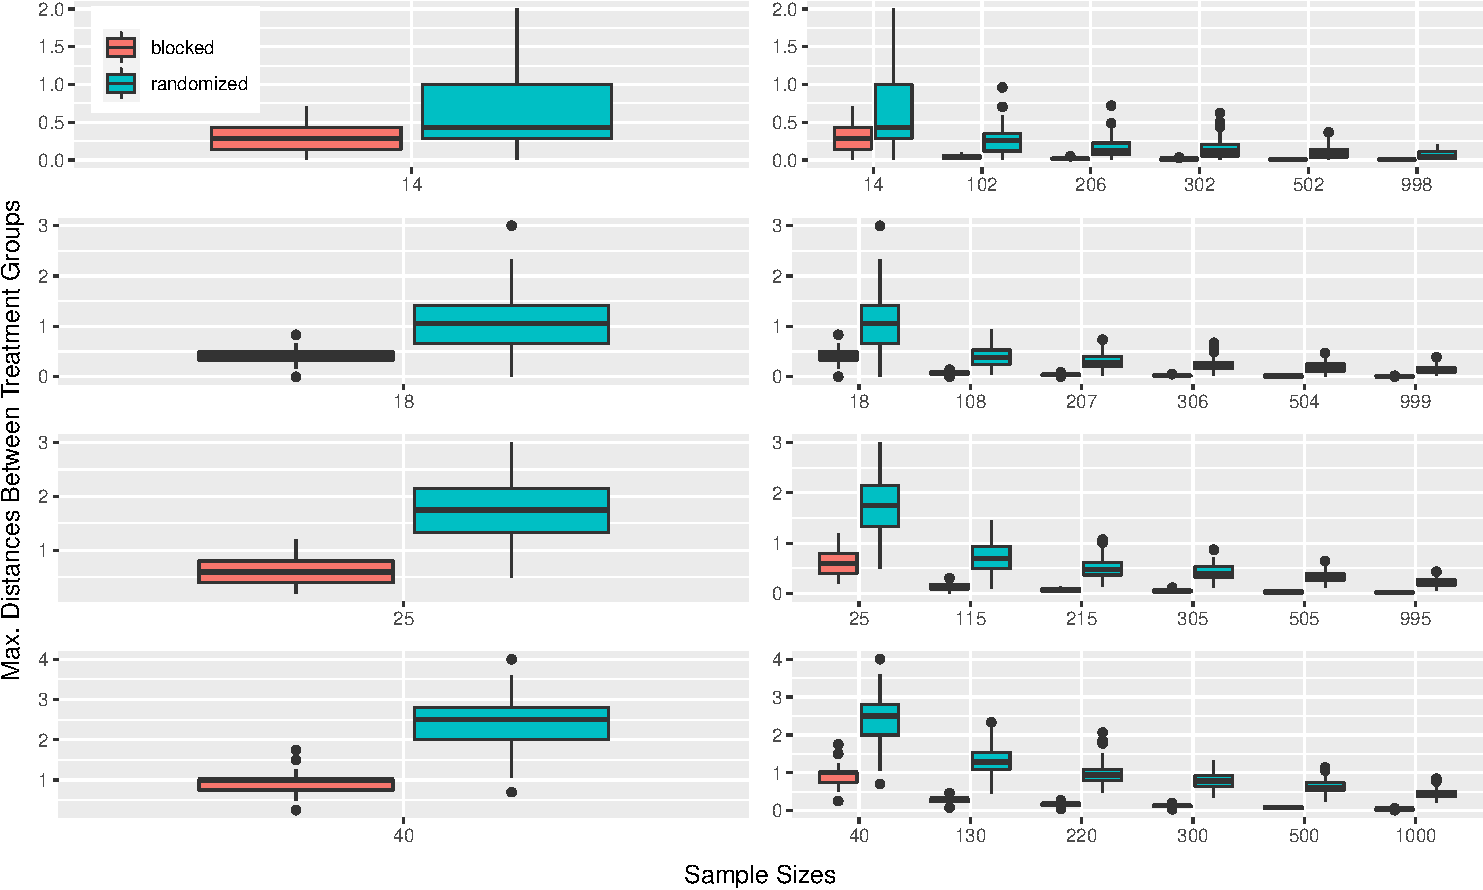
\includegraphics{dissertation_files/figure-latex/Boxplot-Law-Large-Numbers-1.pdf}
\caption{\label{fig:Boxplot-Law-Large-Numbers}Distances between treatment group means in randomized and blocked data. Increasing sample size for 2 (top row), 3 (second row), 5 (third row), and 10 treatment groups (bottom row). Leftmost pair on right panel is exactly the pair on the left panel\label{BoxLawLarNum}}
\end{figure}
For \(n = 998\) and two treatment groups, the largest distance between randomized treatment groups is 0.208, and the largest distance between blocked treatment groups is 0.01. For small samples and a large number of treatment groups, however, the difference is much starker. For \(n = 40\) and ten treatment groups, the largest distance between randomized treatment groups is 4, and the largest distance between blocked treatment groups is 1.75. Figure \ref{HistLawLarNum} shows the distribution of these imbalances.
\begin{figure}
\centering
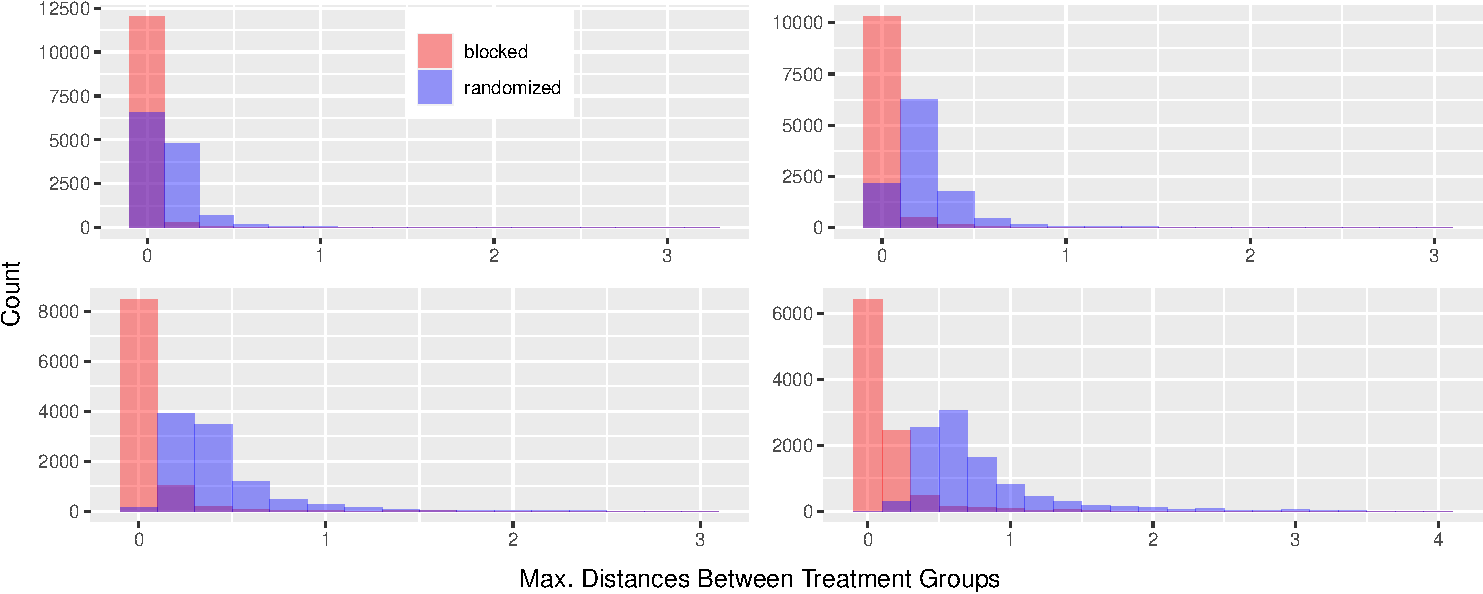
\includegraphics{dissertation_files/figure-latex/Hist-Law-Large-Numbers-1.pdf}
\caption{\label{fig:Hist-Law-Large-Numbers}Distribution of treatment group differences in randomized and blocked data for 2 (top left), 3 (top right), 5 (bottom left), and 10 (bottom right) treatment groups\label{HistLawLarNum}}
\end{figure}
\hypertarget{ordblock-theory-blocking-onthego}{%
\subsubsection{Blocking On The Go}\label{ordblock-theory-blocking-onthego}}

In political science, researchers often have an already-collected data set in front of them. One example would be the American National Election Studies (ANES), a pre-existing survey database, which is often used to analyze voter turnout (see for instance Jackman \& Spahn, 2018; Leighley \& Nagler, 2014), among many others. This setup means all covariate information on all participants is known at the time of assignment, which makes blocking straight-forward. Oftentimes, however, the covariate information of all participants is not known at the time of assignment. This is the case, for instance, for online survey experiments, where each participant completes the survey at differing times. Participants `trickle in' for treatment assignment as the experiment progresses. `Traditional' blocking can not be used here, since it relies on covariate information about the entire sample. Instead, we need to block continuously as the experiment progresses, or block `on the go'. This is called sequential blocking.

Sequential blocking in political science is based on covariate-adaptive randomization, which varies probabilities based on knowledge about previous participants and the current participant (Chow \& Chang, 2007). Traditional covariate-adaptive approaches, such as the biased coin design (Efron, 1971) and minimization (Pocock \& Simon, 1975), assign the incoming participant to the treatment group with the fewest participants with identical covariate information. This works for discrete covariates as the number of possible covariate levels is finite. For continuous covariates, the number of possible covariate levels rises exponentially. Participants are unlikely to look the same, and identical participants are rare. Blocking on continuous covariates is not possible with these traditional approaches (Eisele, 1995; Markaryan \& Rosenberger, 2010; Rosenberger \& Lachin, 2002). Moore \& Moore (2013) develop a method to do so by exploiting relationships between the current participant's covariate profile and those of all previously assigned participants. They define the similarity between participants with the Mahalanobis distance (MD) between participants \(q\) and \(r\) with covariate vectors \(\bm{x}_q\) and \(\bm{x}_r\), \newline \noindent \(MD_{qr} = \sqrt{(\bm{x}_q - \bm{x}_r)' \reallywidehat{\sum}^{-1} (\bm{x}_q - \bm{x}_r)}\). To aggregate pairwise similarity, they implement the mean, median, and trimmed mean of the pairwise MDs between the current participant and the participants in each treatment condition: Participants are indexed with treatment condition \(t\) using \(r \in \{1,...,R\}\). For each condition \(t\), an average MD between the current participant, \(q\), and the participants previously assigned, \(t\). If the distance in terms of MD for the incoming participant is 2 in the control and 5 for the treatment condition, the incoming participant looks more similar to the control condition. To set the probability of assignment, Moore \& Moore (2013) calculate the mean Mahalanobis distances for each incoming participant, \(q\), for all treatment conditions, \(t\), and sort the treatment conditions by these averages. Randomization is biased towards conditions with high scores. For each value of \(k\), with \(k \in \{2,3,...,6\}\), the condition with the highest average MD is then assigned a probability \(k\) times larger than all other assignment probabilities.

Blocking is thus possible when all covariate information is known at the time of assignment and when this information `trickles in' over time. Covariate information, however, is only one side of the coin. Researchers also need to take into consideration the characteristics of the variable to block on. Not all types of variables can and should be used the same way to be blocked on. Specifically, the current use of ordinal variables as blocking variables is somewhat problematic. I describe these problems and my proposed solution in section \ref{intro} above. The following section will apply this solution to differing types of data.

\hypertarget{ordblock-data}{%
\section{Data}\label{ordblock-data}}

One of the most respected and recognized externally and internally valid data sets are the American National Election Studies. I thus choose the following ordered probit model with the 2016 ANES data (the predictors are standard linear predictors in political science literature):

\vspace{-1cm}

\[Education \sim Gender + Race + Age + Income + Occupation + Party ID\]

When trained on the 2016 ANES data, this ordinal probit model estimates the thresholds between each of the education categories shown in Table \ref{education-categories}.
\begin{table}[!htbp] \centering 
  \caption{Ordered Probit Threshold Estimates} 
  \label{education-categories} 
\begin{tabular}{@{\extracolsep{5pt}} D{.}{.}{-3} D{.}{.}{-3} D{.}{.}{-3} D{.}{.}{-3} } 
\\[-1.8ex]\hline 
\hline \\[-1.8ex] 
\multicolumn{1}{c}{Thresholds} & \multicolumn{1}{c}{Coefficients} & \multicolumn{1}{c}{Standard Errors} & \multicolumn{1}{c}{t-values} \\ 
\hline \\[-1.8ex] 
\multicolumn{1}{c}{Up to 1st\textbar 1st-4th} & -7.869 & 1.024 & -7.681 \\ 
\multicolumn{1}{c}{1st-4th\textbar 5th-6th} & -7.146 & 0.717 & -9.965 \\ 
\multicolumn{1}{c}{5th-6th\textbar 7th-8th} & -5.379 & 0.326 & -16.515 \\ 
\multicolumn{1}{c}{7th-8th\textbar 9th} & -4.671 & 0.253 & -18.472 \\ 
\multicolumn{1}{c}{9th\textbar 10th} & -3.920 & 0.206 & -19.070 \\ 
\multicolumn{1}{c}{10th\textbar 11th} & -3.468 & 0.188 & -18.489 \\ 
\multicolumn{1}{c}{11th\textbar 12th} & -2.984 & 0.174 & -17.100 \\ 
\multicolumn{1}{c}{12th\textbar HS grad} & -2.511 & 0.166 & -15.116 \\ 
\multicolumn{1}{c}{HS grad\textbar Some college} & -0.711 & 0.154 & -4.607 \\ 
\multicolumn{1}{c}{Some college\textbar Associate} & 0.384 & 0.154 & 2.500 \\ 
\multicolumn{1}{c}{Associate\textbar Bachelor's} & 1.045 & 0.154 & 6.766 \\ 
\multicolumn{1}{c}{Bachelor's\textbar Master's} & 2.478 & 0.160 & 15.538 \\ 
\multicolumn{1}{c}{Master's\textbar Professional} & 4.099 & 0.177 & 23.144 \\ 
\multicolumn{1}{c}{Professional\textbar Doctorate} & 4.838 & 0.197 & 24.589 \\ 
\hline \\[-1.8ex] 
\end{tabular} 
\end{table}
The observations in the data are binned according to the estimated threshold coefficients, which in turn determines what education categories make sense, given the underlying latent continuous variable. Figure \ref{BarEducCat} shows the distribution of both the original and the model-estimated education categories.
\begin{figure}
\centering
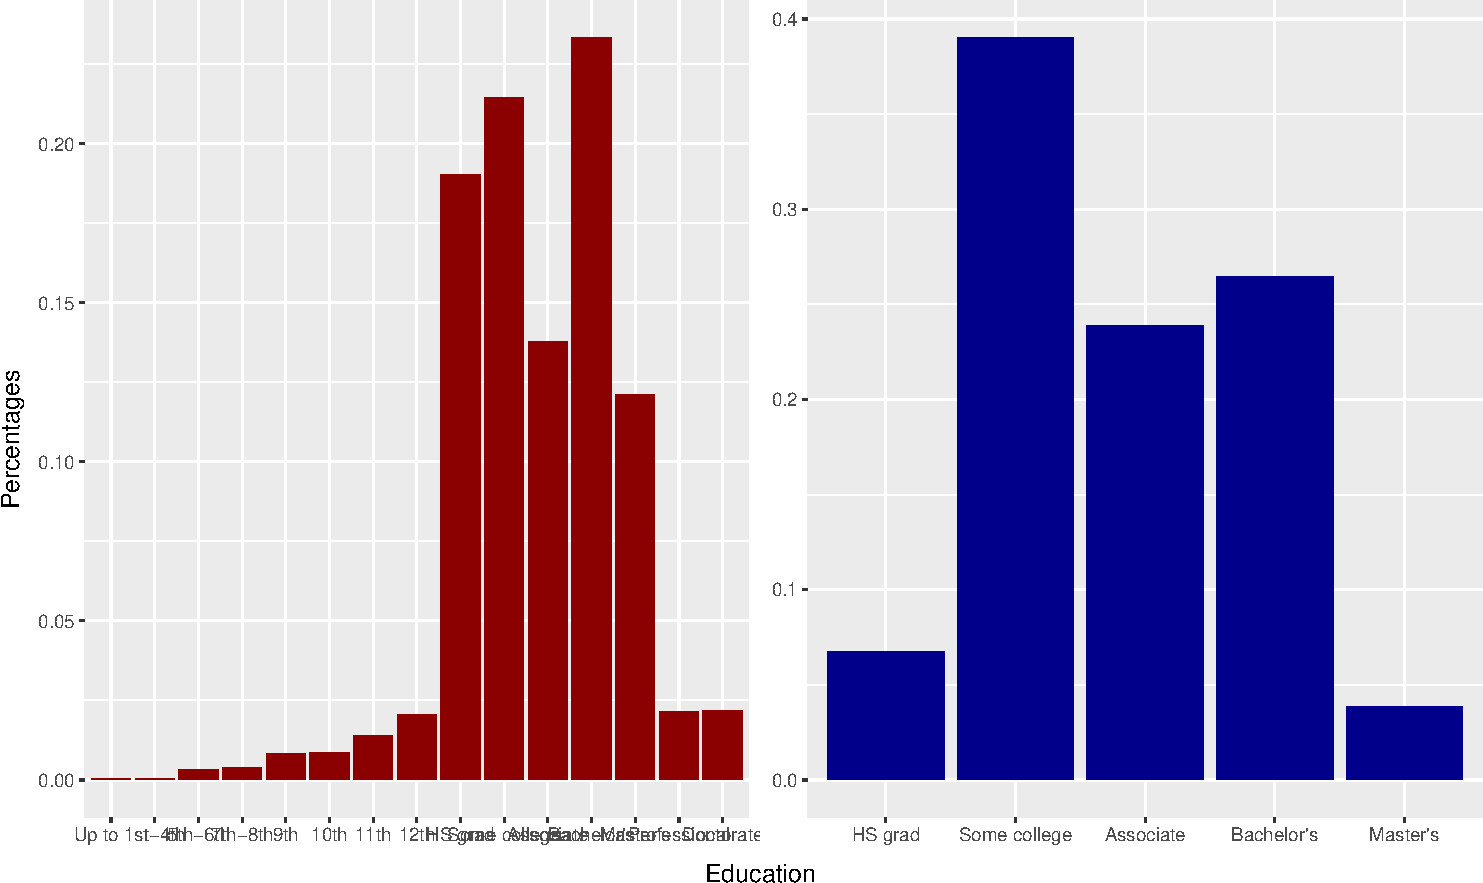
\includegraphics{dissertation_files/figure-latex/Barplot-Education-Categories-1.pdf}
\caption{\label{fig:Barplot-Education-Categories}Distribution of Education Categories. Original 2016 ANES categories on the left, ordered probit estimated categories on the right\label{BarEducCat}}
\end{figure}
As we can see, all categories `below' ``High school graduate'' and `above' ``Master's'' are collapsed because they do not fit the data. The ordered probit model uses the ordinal information with unevenly spaced distances provided and returns categories that do fit the data. We can now use these estimated education categories as the basis for blocking. Assigning numeric values to the new categories is now justifiable because they are based on data-driven estimations. This allows us to block on numerical values with the Mahalanobis distance, which would not be possible without empirical justification. The following sections show that the new estimated categories significantly affect analyses and results.

\hypertarget{ordblock-data-sims}{%
\subsection{Simulations}\label{ordblock-data-sims}}

I conduct various simulations to compare the Ordered Probit Model and its resulting reestimated education categories with the original ANES categories.

\hypertarget{ordblock-data-plac}{%
\subsection{Placebo Regression}\label{ordblock-data-plac}}

We separately block the 2016 ANES on the original and the ordered probit education categories into two treatment groups. We then model the following OLS regression on an interval response variable, a feeling thermometer towards Donald Trump as the Republican presidential candidate:

\vspace{-1cm}

\[Feel.Trump \sim Group + Dem + Rep + Income + Male + White + Black + Hispanic\]

\texttt{Group} indicates a placebo treatment, as no actual treatment is administered. In the absence of actual treatment, the difference between both treatment groups should thus be zero.

\hypertarget{ordblock-data-framing}{%
\subsection{Framing Survey}\label{ordblock-data-framing}}

\hypertarget{ordblock-results}{%
\section{Results}\label{ordblock-results}}

\hypertarget{ordblock-results-sims}{%
\subsection{Simulations}\label{ordblock-results-sims}}

\hypertarget{ordblock-results-plac}{%
\subsection{Placebo Regression}\label{ordblock-results-plac}}

To test this, each blocking/regression process for each set of categories is repeated 1,000 times. The distribution of the placebo treatment indicator (\texttt{Group}) is visualized in Figure \ref{DensPlacTreat}.
\begin{figure}
\centering
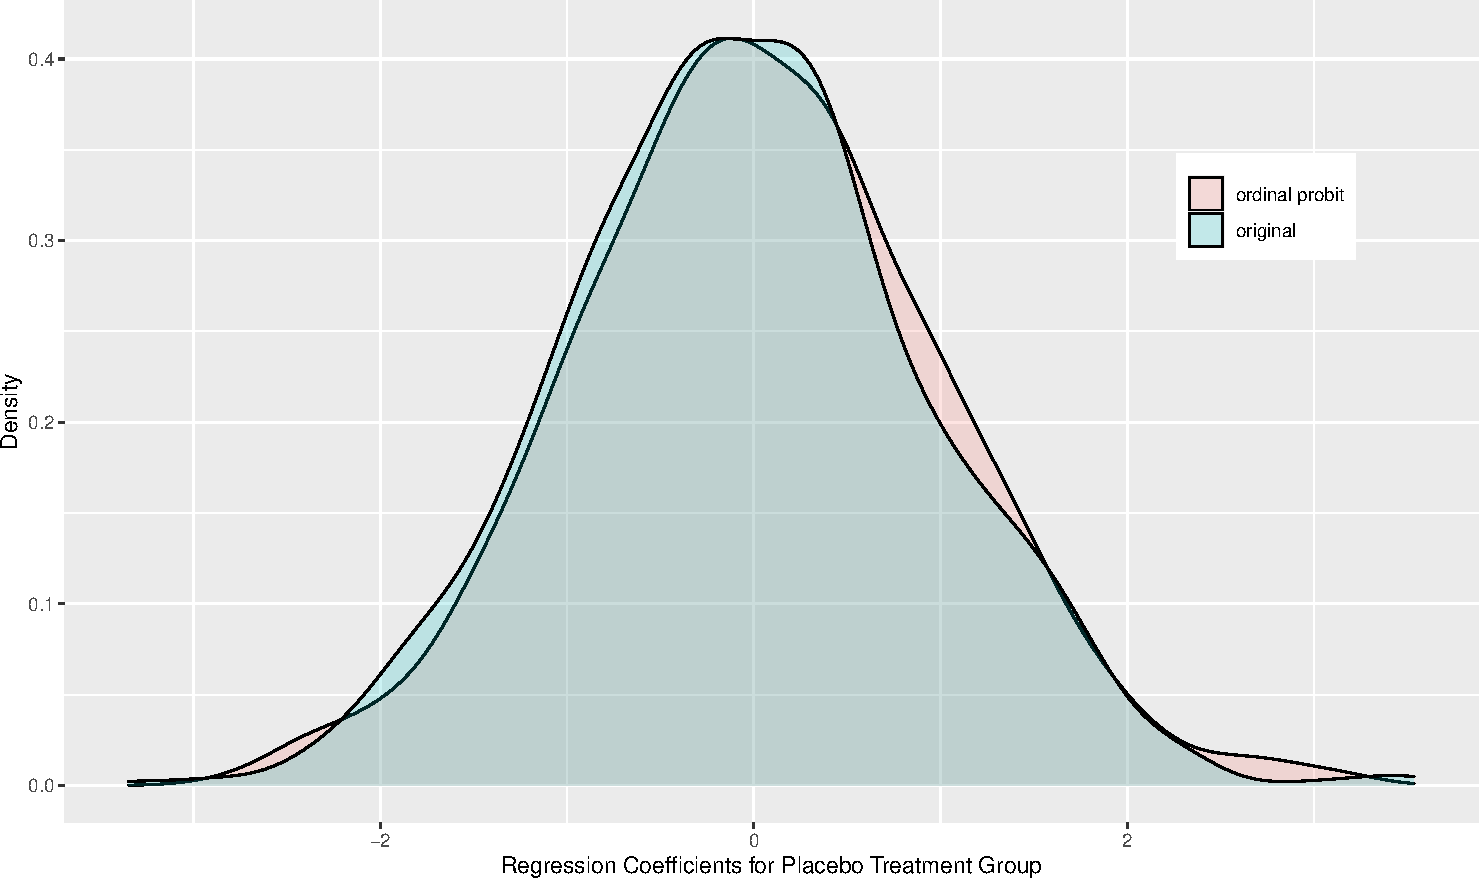
\includegraphics{dissertation_files/figure-latex/Density-Plot-Placebo-Treatment-1.pdf}
\caption{\label{fig:Density-Plot-Placebo-Treatment}Distribution of placebo treatment coefficients by education model\label{DensPlacTreat}}
\end{figure}
Both distributions center around zero, as is the statistical expectation. Upon closer inspection, the ordered probit categories are closer to the true values than the original categories on both mean (-0.05 v. 0.019) and median (-0.07 v. -0.01). This indicates slightly superior performance by the ordered probit categories.

\hypertarget{ordblock-results-framing}{%
\subsection{Framing Survey}\label{ordblock-results-framing}}

Put text here

\hypertarget{ordblock-conclusion}{%
\section{Conclusion}\label{ordblock-conclusion}}

\hypertarget{ordmiss}{%
\chapter{QUALITY COMPARISON OF MAJOR MISSING DATA SOLUTIONS WITH A PROPOSED NEW METHOD FOR ORDINAL VARIABLES}\label{ordmiss}}

\hypertarget{ordmiss-intro}{%
\section{Introduction}\label{ordmiss-intro}}

Missing data are ubiquitous in survey research (Allison, 2002; Raghunathan, 2016). Respondents frequently refuse to answer questions, select ``Don't Know'' as a response option, or drop out during the response collection process (Honaker \& King, 2010). This poses a big problem for researchers because data can typically not be analyzed with statistical software if they contain missing values (Little \& Rubin, 2002; Molenberghs \& Kenward, 2007). Scholars have developed several ways to treat missing data. These can be roughly categorized into deletion, single imputation, and multiple imputation. Single imputation concerns the replacement of missing values with substitute estimates such as the mean, regression coefficients, or values from randomly drawn `similar' respondents in the data. Multiple imputation estimates missing values from conditional distributions and subsequently averages the results into a single parameter of inference (Fay, 1996; King, Honaker, Joseph, \& Scheve, 2001; Rubin, 1976).

Multiple imputation has become the state of the art in missing data management since it accounts for and incorporates uncertainty around the estimated imputations through repeated draws (Andridge \& Little, 2010; Graham \& Schafer, 1999; Schafer \& Graham, 2002; White, Royston, \& Wood, 2011). This is missing from single imputation techniques which treat the single estimated replacement value as a de-facto data entry on par with observed values. Uncertainty is not reflected in the imputed values, which leads to biased standard errors and confidence intervals (Gill \& Witko, 2013; Kroh, 2006). Similarly, listwise deletion has been shown to induce bias with political data (Bodner, 2008; Collins, Schafer, \& Kam, 2001; Pigott, 2001; Rees \& Duke-Williams, 1997; Reilly, 1993).

However, parametric multiple imputation as applied by the most popular imputation packages in \texttt{R} is not necessarily always the most suitable method for all types of variables. For discrete data, multiple hot deck imputation, a combination of the single imputation method hot decking (see section \ref{ordmiss-theory-impute-hd}) and multiple imputation, proves more precise as it avoids the common multiple imputation technique of imputing discrete data on a continuous scale (Gill \& Cranmer, 2012). This practically turns discrete variables into continuous variables which changes their nature and can result in non-observable and biased imputation values with artificially smaller standard errors (Fuller \& Kim, 2005; Kim, 2004; Kim \& Fuller, 2004). Multiple hot deck imputation on the other hand preserves the integrity of discrete data, does not change the size of standard errors, and produces more accurate imputations. It estimates affinity scores for each missing value to measure how similar a respondent with a missing value is to another respondent across all variables except the missing one.

However, multiple hot deck imputation does not account for ordinal variables as its affinity score algorithm assumes even distances between categories in discrete data. This assumption does not apply for ordinal variables. I propose a method designed to impute discrete missing data specifically from ordinal variables. Because of the success of multiple hot deck imputation in its applicability to missing data with discrete variables with a small number of categories (Gill \& Cranmer, 2012), this method is based on multiple hot deck imputation and adapted to account for the specific circumstances of ordinal variables. Based on the ordered probit model approach described in section \ref{intro-op}, it applies a scaled solution with newly estimated numeric thresholds from an assumed underlying latent continuous variable to measure the distances between the categories and calculate affinity scores.

The following is an outline of the remainder of this chapter: Sections \ref{ordmiss-theory-mechanisms} to \ref{ordmiss-theory-singimpute} will discuss the theory behind missing data mechanisms and provide an overview of listwise deletion as well as the most common single imputation methods. Section \ref{ordmiss-theory-multimpute} explains the basics of multiple imputation and outlines major \texttt{R} packages that implement it. These include \texttt{Amelia}, \texttt{mice}, \texttt{hot.deck} (applying multiple hot deck imputation), and my self-penned multiple hot deck imputation function for ordinal variables, \texttt{hd.ord}. Since single imputation is widely condemned as a general imputation method, my focus lies on multiple imputation. Section \ref{ordmiss-data} describes the survey data these packages/functions are tested on: A selection of the 2016 ANES and a subset of the 2016 CCES. Each dataset is complete and randomly amputed to insert missing data. Each of the four \texttt{R} packages/functions is applied to each dataset and tested for accuracy and speed for different types of missingness (MAR, MNAR) and variables (nominal, ordinal, interval). Section \ref{ordmiss-results} shows the results and assesses the usefulness of my proposed new method. Finally, section \ref{ordmiss-conclusion} will feature concluding remarks.

\hypertarget{ordmiss-theory}{%
\section{Theory}\label{ordmiss-theory}}

\hypertarget{ordmiss-theory-mechanisms}{%
\subsection{Missing Data Mechanisms}\label{ordmiss-theory-mechanisms}}

Let there be \(Y\), an \(n \times v\) matrix with data on \(n\) respondents for \(v\) variables. Let there also be the response indicator \(R\) as an \(n \times v\) matrix with values of 0 or 1. Let their respective elements be denoted by \(y_{ij}\) and \(r_{ij}\), with \(i = 1, ..., n\) and \(j = 1, ..., v\). If \(y_{ij}\) is observed, \(r_{ij} = 1\). If \(y_{ij}\) is missing, \(r_{ij} = 0\). All elements where \(r_{ij} = 0\) make up the missing data, \(Y^{miss}\). All elements where \(r_{ij} = 1\) make up the observed data, \(Y^{obs}\). Together, \(Y^{obs}\) and \(Y^{miss}\) form the complete data \(Y\). Missing data can then generally be described by \(\text{prob}(R = 0 | Y^{obs}, Y^{miss}, \beta)\), i.e.~the probability of missing data depends on the observed data, the missing data, and a vector of unknown parameters.\footnote{The literature often uses \(\theta\) for missing data notation, but since my concern lies primarily with regression style models, I will be using \(\beta\) instead.} Depending on the mechanism by which data is missing, this expression can be further simplified.

Data can be missing by three basic mechanisms: It can be missing completely at random (MCAR), missing at random (MAR), or missing not at random (MNAR). It is not possible to test respective data on the mechanism underlying their missingness. The onus here is on the researcher to make substantive assumptions based on the nature of the data at hand -- in other words: Researchers need to make assumptions about how the data came to be missing in the first place.

The simplest and easiest case is missing completely at random (MCAR). Under the MCAR assumption, there is no process guiding the missingness; it is inserted truly at random. In statistical terms, this means both the unobserved and the missing data independently from each other form a random sample of the population and have the same underlying distribution. Missing data would not pose such a serious problem, if it routinely and ubiquitously occurred MCAR. Unfortunately, however, that is not the case, even when restricted to survey data: Survey respondents are known to withhold sensitive data (Groves et al., 2009). This can stretch from the unwillingness to divulge information deemed to be personally private (income, sexual orientation) to the refusal to answer sensitive questions out of fear of political or social repercussions in the community (union membership, support for polarizing political candidates). These types of missing data occur systematically, e.g.~answers have not been refused randomly across the whole range of income levels but are missing only for respondents with very high or very low income. Similarly, only answers criticizing the authorities are missing in surveys in non-democratic states, while the state-loyal responses are present. Notationally, the general missing data expression can be simplified under the MCAR assumption to \(\text{prob}(R = 0 | \beta)\), i.e.~the generic probability of missing data, independent of the data themselves and only dependent on \(\beta\).

As a result, a MCAR assumption in political science surveys is rare and requires tremendous justification. It is more commonly assumed among researchers that missing data are missing at random (MAR). MAR means missing data are related to the observed but not the unobserved data. In practical terms, this for instance means missing data on income can be related to observed data on education or occupation. Here, the missing data are not a random sample of the entire data. MAR transforms the general missing data expression to \(\text{prob}(R = 0 | Y^{obs}, \beta)\), i.e.~the chances of missing data depend on the observed data and \(\beta\).

Finally, missing data can be missing not at random (MNAR).\footnote{Data MNAR is also sometimes called `non-ignorable' (see for instance Gill \& Cranmer (2012) and Allison (2002)).} This is the case when missing data are related to unknown and/or unobserved parameters. Continuing the example of missing data on income, under MNAR we do not observe data on education or occupation that can be used to fill the missing income data slot. In the case of data MNAR, the general missing data expression remains unchanged, \(\text{prob}(R = 0 | Y^{obs}, Y^{miss}, \beta)\), i.e.~the missingness of data depends on the observed and the missing data.

As mentioned above, it is not possible to test whether missing data is MCAR, MAR, or MNAR. The assessment of the missing data mechanism underlying any respective data comes from researchers and their understanding of the data generating process. The statistical methods to address missing data can be broadly categorized into deletion, imputation, and multiple imputation. Sections \ref{ordmiss-theory-delete} to \ref{ordmiss-theory-multimpute} outline these below. Given the focus of this chapter, special attention lies on section \ref{ordmiss-theory-multimpute}.

\hypertarget{ordmiss-theory-delete}{%
\subsection{Listwise Deletion}\label{ordmiss-theory-delete}}

One of the most common methods of handling missing data in quantitative political science is listwise deletion. This involves the removal of any incomplete observations, thereby reducing the sample size. The resulting sample is then ready for analysis. Whilst almost unbeatable in its simplicity and speed, this method often induces bias, depending on how much data are missing, how non-random the pattern of missingness is, and other aspects (Allison, 2002; King et al., 2001; Little \& Rubin, 2002).

In the case of data MCAR, listwise deletion is not biased, as it removes a random sample of the population (King et al., 2001; Schafer \& Graham, 2002). When missing data are MAR, listwise deletion is always biased, since the observed data is tilted towards respondents with characteristics that make them more likely to respond. Whether this bias is trivial or substantial depends on the research in question (Collins et al., 2001; Graham, Hofer, Donaldson, MacKinnon, \& Schafer, 1997). The potential for severe bias increases with data MNAR (Collins et al., 2001; Diggle \& Kenward, 1994; Glynn, Laird, \& Rubin, 1993; Robins, Rotznitzky, \& Scharfstein, 1998).

While the bias inserted by listwise deletion in each individual data analysis may not necessarily be drastic, studies have shown that it can be so severe as to alter substantive conclusions (Brown, 1994; Graham, Hofer, \& MacKinnon, 1996; Honaker \& King, 2010; Wothke, 2000). Even if that were not or only rarely the case and most data were MCAR, reducing the sample size is generally never a recommended approach as, among other aspects, standard errors from regression models are inflated. As King et al. (2001) put it, the result of listwise deletion ``is a loss of valuable information at best and severe selection bias at worst'' (p.~49). In \texttt{R}, listwise deletion can be implemented with the base function \texttt{na.omit}.

\hypertarget{ordmiss-theory-singimpute}{%
\subsection{Single Imputation}\label{ordmiss-theory-singimpute}}

Single imputation means replacing missing data with substituted values, i.e.~the structural opposite of deletion. Imputation requires some method of creating a predictive distribution, based on the observed data, from which value substitutions are picked. Single imputation, regardless of its exact nature, is not recommended to impute missing data since, similar to deletion, it biases standard errors and confidence intervals (Honaker \& King, 2010). Crucially, uncertainty is not reflected in the imputed values (Little \& Rubin, 2002). The following subsections are mere selections of the most common single imputation methods and make no claim of completeness. Since single imputation is widely condemned as a general imputation method and as my focus lies on multiple imputation, they are also brief.

\hypertarget{ordmiss-theory-impute-mean}{%
\subsubsection{Mean}\label{ordmiss-theory-impute-mean}}

Mean imputation, sometimes also called unconditional mean imputation, means replacing missing values within cells with the mean of the observed values, so \(Y^{miss} = \overline{Y^{obs}}\). While it does not change the mean of the sample, this method distorts the empirical distribution of \(Y\), which in turn produces biased estimates of any non-linear quantities such as variances and covariances (Haitovsky, 1968). It is also bound to be inaccurate in most cases, since few values generally fall exactly on the mean, and can be non-sensical for discrete variables (Efron, 1994).

Mean imputation can be done in many ways in \texttt{R}, for instance with the \texttt{impute} function in the \texttt{Hmisc} package or by setting \texttt{method\ =\ "mean"} in the \texttt{mice} function in the \texttt{mice} package. It is also very simple to execute in base \texttt{R}, e.g.~for a sample data frame \texttt{df} and the numeric column \texttt{x}: \(\text{df} \leftarrow \text{transform(df, x = ifelse(is.na(x), mean(x, na.rm=TRUE), x))}\).

\hypertarget{ordmiss-theory-impute-regress}{%
\subsubsection{Regression}\label{ordmiss-theory-impute-regress}}

Imputation by regression, sometimes also called conditional mean imputation, imputes missing values conditional on observed values. Researchers predict observed variable values based on other variables, while the fitted values from the regression model are then used to impute variable values where they are missing. Let there be an independent variable \(x\) in a multiple regression model. Assume that \(x\) contains missing values, \(x^{miss}\), and observed values, \(x^{obs}\). We regress \(x^{obs}\) on the other independent variables and use the estimated equation to generate predicted values for \(x^{miss}\), \(x^{pred}\). \(x^{pred}\) then replace \(x^{miss}\), thus completing the dataset. While more accurate than mean imputation, particularly for large samples with data MCAR, regression imputation nonetheless suffers from the same flaw that accompanies all single imputation approaches: Uncertainty is not reflected in the imputed values (Horton \& Kleinman, 2007).

Differing variations of imputation by regression exist in \texttt{R}, such as the \texttt{aregImpute} function in the \texttt{Hmisc} package, which performs additive regression, and setting \texttt{method\ =\ "norm.predict"} in the \texttt{mice} function to conduct linear regression. The \texttt{predict} function in base \texttt{R} also applies linear regression imputation.

\hypertarget{ordmiss-theory-impute-hd}{%
\subsubsection{Hot Decking}\label{ordmiss-theory-impute-hd}}

Hot deck imputation was developed in the 1970s and replaces missing values with values from similar respondents in the sample (Ernst, 1978; Ford, 1983). It is called `hot decking' as a reference to taking draws from a deck of matching computer punch-cards. The deck was `hot' since it was currently being processed, as opposed to pre-collected or `cold' data (Andridge \& Little, 2010; Little \& Rubin, 2002). In the most general version, researchers select all respondents that are `similar' to a respondent with missing data and randomly draw one of those respondents (with replacement) to fill in the missing value. The respondent with the initially missing value is termed the \textit{recipient}, while the `similar' respondent is called the \textit{donor}. Variations of the method include hot decking within adjustment cells, by nearest neighbor, and sequentially ordered by a covariate (Cox, 1980; David, Little, Samuhel, \& Triest, 1986; Kaiser, 1983; Kalton \& Kish, 1981; Rockwell, 1975).

Contrary to mean or regression imputation, hot deck imputation preserves the integrity of the data, i.e.~only actually observed values are used to fill in missing slots (Bailar \& Bailar, 1997). In both other single imputation methods, it is possible and sometimes even likely that missing values are replaced by values not found amongst the observed values. Contrary to regression imputation, hot decking also does not require a fitted model and is thus less vulnerable to model misspecification. However, hot decking does necessitate the existence of at least some donors for a respondent at every variable value that is missing. With a lot of missing data and few `similar' matches, the accuracy of hot decking greatly decreases (Young, Weckman, \& Holland, 2011). Hot decking works best for discrete data as continuous data are very unlikely to be matched or `similar', though the definition of what might constitute a `similar' respondent is somewhat subjective (Marker, Judkins, \& Winglee, 2002). As is the case with all single imputation methods, uncertainty is not reflected in the imputed values. Selecting the initial sample of `similar' respondents and the subsequent random sampling from that subsampling is treated as factual responses, which leads to smaller standard errors and confidence intervals than statistically valid (Little \& Rubin, 2002).

To my knowledge, there is currently no \texttt{R} package that applies single hot deck imputation. Nonetheless, variations of hot decking are still in use by some government statistics agencies such as the National Center for Education Statistics (for parts of the Current Population Survey) or the U.S. Bureau of the Census (NCES, 2002; USBC, 2002).

\hypertarget{ordmiss-theory-multimpute}{%
\subsection{Multiple Imputation}\label{ordmiss-theory-multimpute}}

Multiple imputation was invented by Rubin in the 1970s to account for the absence of uncertainty in single imputation methods and allow more accurate standard error estimates. It fills missing values with a predictive model that includes observed data and prior knowledge (Honaker \& King, 2010). Over the time of its development, it has become the dominant sophisticated strategy for handling missing data (Dempster, Laird, \& Rubin, 1977; Glynn et al., 1993; Heitjan \& Rubin, 1991; Little \& Rubin, 2002; Rubin, 1976, 1987, 1996; Rubin \& Schenker, 1986). Multiple imputation involves three general steps:
\begin{enumerate}
\def\labelenumi{(\arabic{enumi})}
\item
  Impute a dataset with missing values \(m\) times. This results in \(i\) complete datasets (with \(i = 1, ..., m\))
\item
  Analyze each of the \(i\) complete datasets
\item
  Combine the results from each of the \(i\) analysis results into one collective result
\end{enumerate}
\vspace{0.8cm}

\ssp
\begin{figure}[ht]
\centering
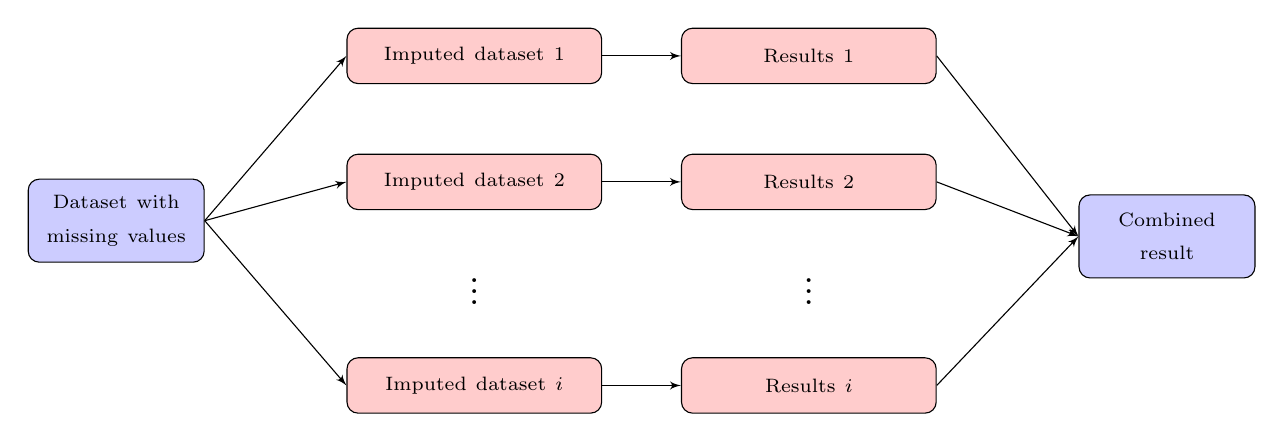
\begin{tikzpicture}
    \node [block3] (ds) {\scriptsize{Dataset with missing values}};
    \node [block2r, above right=1.2cm and 1.8cm of ds] (imp1) {\scriptsize{Imputed dataset 1}};
    \node [block2r, above right=-0.4cm and 1.8cm of ds] (imp2) {\scriptsize{Imputed dataset 2}};
    \node [block2r, below right=1.2cm and 1.8cm of ds] (impi) {\scriptsize{Imputed dataset $i$}};
    \coordinate[right=0cm of ds] (dsc);
    \coordinate[left=0cm of imp1] (imp1lc); 
    \coordinate[left=0cm of imp2] (imp2lc); 
    \coordinate[left=0cm of impi] (impilc); 
    \path [line] (dsc) -- (imp1lc);
    \path [line] (dsc) -- (imp2lc);
    \path (imp2) --node[auto=false]{\Large{\vdots}} (impi);
    \path [line] (dsc) -- (impilc);
    \node [block2r, right=1cm of imp1] (results1) {\scriptsize{Results 1}};
    \node [block2r, right=1cm of imp2] (results2) {\scriptsize{Results 2}};
    \node [block2r, right=1cm of impi] (resultsi) {\scriptsize{Results $i$}};
    \coordinate[right=0cm of imp1] (imp1rc);
    \coordinate[right=0cm of imp2] (imp2rc);
    \coordinate[right=0cm of impi] (impirc);
    \coordinate[left=0cm of results1] (results1lc); 
    \coordinate[left=0cm of results2] (results2lc); 
    \coordinate[left=0cm of resultsi] (resultsilc); 
    \path [line] (imp1rc) -- (results1lc);
    \path [line] (imp2rc) -- (results2lc);
    \path (results2) --node[auto=false]{\Large{\vdots}} (resultsi);
    \path [line] (impirc) -- (resultsilc);
    \node [block3, below right=1.4cm and 1.8cm of results1] (results) {\scriptsize{Combined result}};
    \coordinate[left=0cm of results] (resultsc);
    \coordinate[right=0cm of results1] (results1rc);    
    \coordinate[right=0cm of results2] (results2rc);    
    \coordinate[right=0cm of resultsi] (resultsirc);    
    \path [line] (results1rc) -- (resultsc);
    \path [line] (results2rc) -- (resultsc);
    \path [line] (resultsirc) -- (resultsc);
\end{tikzpicture}
\caption{Multiple Imputation Workflow} 
\label{mi-workflow}
\end{figure}
\dsp

Figure \ref{mi-workflow} provides a graphical overview of this workflow. Each missing value is imputed \(m\) times from a conditional distribution using other present values for the respective value to create \(i\) imputed complete datasets. The chosen statistical analysis \(\tau\), for instance a regression model, is applied to each of these \(i\) datasets, resulting in \(\tau_{i}\), with \(i = 1, ..., m\). Averaging \(\tau_{i}\) then gives us the single estimate, \(\overline{\tau}\). Together, this is expressed as:
\begin{align}
\overline{\tau} = \frac{1}{m}\sum\limits_{i=1}^{m} \tau_{i}.
\end{align}
Following Rubin (1987), the total variance of \(\overline{\tau}\), \(Var_T\) consists of the mean variance of \(\tau_i\) within each dataset \(i\), \(\overline{Var_W}\), and the sample variance of \(\tau\) across both datasets, \(Var_A\):
\begin{align}
\overline{Var_W} &= \frac{1}{m} \sum\limits_{i=1}^{m} SE(\tau_i)^2\\
Var_A &= \sum\limits_{i=1}^{m} \frac{(\tau_{i} - \overline{\tau})^2}{m -1}\\
Var_T &= \overline{Var_W} + Var_A
\end{align}
Multiplied by a factor correcting for small numbers of \(m\) (as \(m < \infty\)), \(Var_T\) is adjusted to:
\begin{align}
Var_T = \overline{Var_W} + Var_A (1 + \frac{1}{m})
\end{align}
Each imputed complete dataset is identical to all other imputed complete datasets, with the exception of the imputed value. The imputed values for a missing value differ with each imputation of \(M\) in order to reflect uncertainty levels. The `multiple' part of the imputation is a crucial aspect here since each imputation run will produce slightly different parameter estimates. Imputing multiple times and then averaging the results creates variability which adjusts the standard errors upward (Kroh, 2006). This deliberate random variation included in a deterministic multiple imputation run removes the overconfidence from single imputation, where the standard error estimates are too low (Schafer \& Graham, 2002). In a case where the utilized multiple imputation model predicts missing values well, variation across the imputed values is small. In other cases, variation may be larger, depending on the level of certainty we have about the missing value. Multiple imputation has been shown to produce consistent, asymptotically efficient and normal estimates for a variety of data MAR (Allison, 2002).

Choosing \(m\), the number of imputations, is somewhat subjective. Originally, \(m = 5\) was considered sufficient based on efficiency calculations (Rubin, 1987) and is still the default in most software packages. More recent discussions stress the need for an increase of \(m\) in order to estimate more nuanced standard errors. Various approaches continue to coexist, such as focusing on the parameter with the largest fraction of missing information (Kroh, 2006) or starting with \(m = 5\) and gradually increasing it in subsequent runs (Raghunathan, 2016). The most common current practice appears to be to set \(m\) to the percentage of missing data, i.e.~if 20 percent of data are missing, \(m = 20\) (Bodner, 2008; White et al., 2011).

There are numerous ways to implement multiple imputation. Up until the late 1990s, this required considerable statistical knowledge and sophisticated methodological skills (see Honaker \& King (2010) for an overview). The use of multiple imputation was thus limited to a rather specialized audience of statisticians and methodologists. Since then, numerous \texttt{R} packages have emerged to facilitate user-friendliness. The by far most popular packages are \texttt{mice} and \texttt{Amelia}. Since its inception in 2001, \texttt{mice} has been cited 5,276 times on Google Scholar at the time of writing. \texttt{Amelia} was created in 1998 and has been cited 1,836 times. They are both considered among the very best implementations of multiple imputation (Horton \& Kleinman, 2007). Any improvement in multiple imputation thus needs to be measured against them. \texttt{hot.deck}, the method by Gill \& Cranmer (2012) upon which my proposed method of multiple hot deck imputation with ordinal variables, \texttt{hd.ord} is based, follows this approach and demonstrates improved results when compared to \texttt{Amelia}. My \texttt{hd.ord} analysis extends this and also includes \texttt{mice} as a further benchmark of performance.

The following sections do not cover the full list of functions available in each package, as this would go far beyond the scope of this chapter and could literally fill books of its own, as evidenced by the 182-page package manual for \texttt{mice} (Buuren et al., 2020). Instead, I will focus on the packages' core underlying mechanisms and their major functions to perform imputation, which are named after their package namesakes: \texttt{mice}, \texttt{amelia}, \texttt{hot.deck}, and \texttt{hd.ord}.\footnote{For the remainder of this chapter and to avoid confusion, all names will refer to the function unless explicitly stated otherwise.} I extend the focus on simplicity and user-friendliness further by running these major imputation functions with their default settings. Survey analysts usually do not possess the statistical expertise that enable them to dive deeply into distribution or chain properties. The vast majority of users can be assumed to use imputation functions with their default settings, particularly when applied to surveys and survey experiments that cover a nationally representative population sample. If a package only proved superior over others by setting specific and highly technical function arguments, this would defeat the purpose of making multiple imputation the missing data approach for the masses. I apply only two very minor exceptions to the default settings: The number of imputations is set to the percentage of missingness instead of the default five, and the console printing options are turned off.

\hypertarget{ordmiss-theory-multimpute-mice}{%
\subsubsection{\texorpdfstring{\texttt{mice}: Multivariate Imputation by Chained Equations}{mice: Multivariate Imputation by Chained Equations}}\label{ordmiss-theory-multimpute-mice}}

The \texttt{R} package \texttt{mice} was released in 2001 (Buuren \& Oudshoorn, 2000). It stands for Multiple Imputation by Chained Equations (MICE), which means imputing incomplete multivariate data by full conditional specification (Buuren, 2007; Buuren \& Groothuis-Oudshoorn, 2011), a version of the imputation-posterior (IP) (King et al., 2001). Full conditional specification refers to imputation on a variable-by-variable basis, i.e.~a set of conditional densities is used to impute data for each individual missing value. This approach does not require the specification of a multivariate distribution for the missing data, which separates it from competing methods like joint modeling (Schafer, 1997). The initial release of \texttt{mice} featured predictor selection, passive imputation, and automatic pooling. Subsequent releases included functionality for imputing multilevel data, post-processing imputed values, specialized pooling, stable imputation of categorical data, and model selection, among many others. Imputation by chained equations is extensively used across domains (see Buuren \& Groothuis-Oudshoorn (2011) for a list of over 20 applied fields).

Chained equations are based on the Gibbs sampler, a randomized Markov chain Monte Carlo algorithm to estimate a sequence of observations from a specified multivariate probability distribution (Gelman et al., 2013; Gill, 2014). In essence, chained equations fill in missing values through an iterative repetition of univariate procedures that are chained together -- hence the name for the procedure. As the term univariate signifies, specification happens at the variable level, i.e.~each chained equation specifies the imputation model separately for each column of the data. Following deliberations by Rubin (1987) and Buuren \& Groothuis-Oudshoorn (2011), imputation by chained equations takes the missing data generating process into account and maintains data relations as well as the uncertainty about these relations. With these conditions satisfied, the imputation model results in statistically valid and factual imputations. This has been proven empirically under various circumstances, for instance for regression models (Giorgi, Belot, Gaudart, \& Launoy, 2008; Horton \& Kleinman, 2007; Horton \& Lipsitz, 2001), continuous data (Yu, Burton, \& Rivero-Arias, 2007), missing predictor variables (Moons, Donders, Stijnen, \& Harrell, 2006), large surveys (Schunk, 2008), and addressing issues of convergence (Brand, 1999; Buuren, Brand, Groothuis-Oudshoorn, \& Rubin, 2006; Drechsler \& Rassler, 2008).

Continuing the notation from section \ref{ordmiss-theory-mechanisms} and incorporating Buuren \& Groothuis-Oudshoorn (2011), let there be \(Y\), an \(n \times v\) matrix with data on \(n\) respondents for \(v\) variables, that is formed of missing, \(Y^{miss}\), and observed data, \(Y^{obs}\). As before, let there also be a vector of unknown parameters \(\beta\). Now let \(Y\) further be a random sample from the \(z\)-variate multivariate distribution, \(Z(Y | \beta)\), with \(\beta\) accounting for the multivariate distribution of \(Y\). The proverbial pot of gold here is how to estimate the multivariate distribution of \(\beta\). Under the chained equations model, we estimate a posterior distribution of \(\beta\) by sampling repeatedly from conditional distributions, i.e.:
\begin{align}
Z(Y_1 &| Y_{-1}, \beta_1) \nonumber\\
&\vdots \nonumber\\
Z(Y_z &| Y_{-z}, \beta_z)
\end{align}
Any iteration \(n\) of chained equations is then a Gibbs sampler that sequentially draws
\begin{align}
\beta_1^{\sim(n)} &\sim Z(\beta_1 | Y_1^{obs}, Y_2^{(n-1)}, ..., Y_z^{(n-1)}) \nonumber\\
Y_1^{\sim(n)} &\sim Z(Y_1 | Y_1^{obs}, Y_2^{(n-1)}, ..., Y_z^{(n-1)}, \beta_1^{\sim(n)}) \nonumber\\
&\vdots \nonumber\\
\beta_z^{\sim(n)} &\sim Z(\beta_z | Y_z^{obs}, Y_1^{(n)}, ..., Y_{z-1}^{(n)}) \nonumber\\
Y_z^{\sim(n)} &\sim Z(Y_z | Y_z^{obs}, Y_1^{(n)}, ..., Y_z^{(n)}, \beta_z^{\sim(n)})
\end{align}
with the chain starting from a random draw from observed marginal distributions and \(Y_i^{(n)} = (Y_i^{obs}, Y_i^{\sim(n)})\) being the \(i\)th imputed variable at iteration \(n\). Note that immediately preceding imputations, \(Y_i^{\sim(n-1)}\), do not affect \(Y_i^{\sim(n)}\) directly but only through connections with other variables.

Figure \ref{mice-func} shows the package's main imputation function, \texttt{mice}, with all its arguments. As stated above, I will use \texttt{mice} with its default settings to ensure simplicity and user-friendliness.
\begin{figure}[hbt]
  \centering
  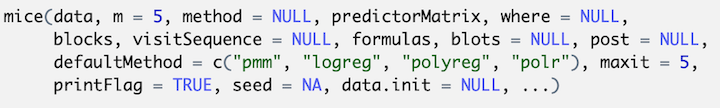
\includegraphics{figures/mice.png}
  \caption{The \texttt{mice} function}
  \label{mice-func}
\end{figure}
The majority of arguments are not of importance to general users. Arguments like \texttt{predictorMatrix}, which specifies the set of predictors to be used for each target column, and \texttt{blocks}, which provides the option to manually put variables into imputation blocks, require too much statistical knowledge to be of use to non-specialists. Other arguments do not affect the basic workings of the function. This applies for instance to \texttt{printFlag}, which sets the console printing preference, \texttt{seed}, which is used to offset the random number generator, and \texttt{data.init}, which specifies a data frame to be used to initialize imputations before the start of the iterative process.

The only important arguments for general users are \texttt{data}, \texttt{m}, and \texttt{defaultMethod}. Only \texttt{data} requires user input. As mentioned above, \texttt{m} should also be set to the percentage of missing data. The argument \texttt{defaultMethod} does not require user input but is crucial for insights into the default workings of \texttt{mice}. Its options \texttt{pmm}, \texttt{logreg}, \texttt{polyreg}, and \texttt{polr} refer to the default imputation methods that are implemented depending on the type of variable in question. The argument \texttt{pmm} (predictive mean matching) is used for numeric data, \texttt{logreg} (logistic regression imputation) for binary and factor data with two levels, \texttt{polyreg} (polytomous regression imputation) for factor data with more than two unordered levels, and \texttt{polr} (proportional odds model) for factor data with more than two ordered levels. Note that \texttt{mice} thus distinguishes between ordered and unordered as well as the number of factor levels, but does not specifically incorporate ordinal variables, which feature ordered but unevenly spaced levels.

\hypertarget{ordmiss-theory-multimpute-amelia}{%
\subsubsection{\texorpdfstring{\texttt{Amelia}: A Program for Missing Data}{Amelia: A Program for Missing Data}}\label{ordmiss-theory-multimpute-amelia}}

The \texttt{R} package \texttt{Amelia} was originally released in 1998 (Honaker, Joseph, King, Scheve, \& Singh, 1998). A second version, \texttt{Amelia\ II}, was released in 2010 (Honaker, King, \& Blackwell, 2012). Contrary to \texttt{mice}, which is based on IP, both versions of \texttt{Amelia} are based on the expectation-maximization (EM) algorithm (Dempster et al., 1977; Gelman et al., 2013; Jackman, 2000; McLachlan \& Krishan, 1997; Tanner, 1996). EM functions to a large part like IP, with the crucial exception that deterministic calculations of posterior means replace random draws from the entire posterior. This translates into running regressions to estimate the regression coefficient􏰒, imputing a missing value with a predicted value, re-estimating the regression coefficient, and repeating the process until convergence (King et al., 2001). While the iterations and parameters thus represent an entire density in IP, they are single maximum posterior values in EM. This makes EM comparatively much faster in finding the maximum of the likelihood function. On its own, however, EM is unsuitable for multiple imputation as it does not provide the rest of the distribution. The \texttt{Amelia} package circumvents this issue with expectation-maximization importance sampling (EMi) (Gelfand \& Smith, 1990; Rubin, 1987; Wei \& Tanner, 1990), which combines EM with the iterative simulation approach of importance sampling. This proved unsuitable for large datasets, however, as it led to high running times and system crashes. The \texttt{Amelia\ II} package addresses this by mixing EM with bootstrapping (Efron, 1994; Lahlrl, 2003; Rubin, 1994; Shao \& Sitter, 1996), allowing the imputation of more variables for more observations more quickly.

\texttt{Amelia\ II} is based on the assumption that the complete data (\(Y^{obs}\) and \(Y^{miss}\)) are multivariate normal (MVN): \(Y \sim N_v(\mu, \sum)\), with mean vector \(\mu\) and covariance matrix \(\sum\). The MVN model has been proven to work for a variety of variable types (Ezzati-Rice et al., 1995; Graham \& Schafer, 1999; Rubin \& Schenker, 1986; Schafer, 1997). Continuing the notation from section \ref{ordmiss-theory-mechanisms} and incorporating Honaker \& King (2010), let there be a vector of unknown parameters \(\beta\), with \(\beta = (\mu, \sum)\). Let there further be our missingness matrix\(R\) and the likelihood of \(Y^{obs}\), \(\text{prob}(Y^{obs}, R | \beta)\). \texttt{Amelia\ II} is explicitly set up for the MAR assumption of missing data, \(\text{prob}(R = 0 | Y^{obs}, \beta)\). Under this assumption, the likelihood can be transformed as
\begin{align}
\text{prob}(Y^{obs}, R | \beta) = \text{prob}(R | Y^{obs}) \text{prob}(Y^{obs} | \beta).
\end{align}
Since the missing mechanism is MAR, we are only interested in the inference on complete data parameters, thus the likelihood becomes
\begin{align}
L(\beta | Y^{obs}) \propto \text{prob}(Y^{obs} | \beta)
\end{align}
which further translates into
\begin{align}
\text{prob}(Y^{obs} | \beta) = \int \text{prob}(Y | \beta) y Y^{miss}
\end{align}
under the law of iterated expectations. This results in the posterior
\begin{align}
\text{prob}(\beta | Y^{obs}) \propto \text{prob}(Y^{obs} | \beta) = \int \text{prob}(Y | \beta) y Y^{miss}.
\end{align}
Taking draws from this posterior is computationally intensive since the contents of \(\mu\) and \(\sum\) increase exponentially as the number of variables increases -- this is the perennial crux of multiple imputation, particularly for large datasets with many variables. \texttt{Amelia\ II} solves this through a combination of EM and bootstrapping. This process bootstraps the data to simulate estimation uncertainty for each posterior draw, runs the EM algorithm to find the mode of the posterior bootstrapped data, and then imputes by drawing from \(Y^{miss}\) conditional on \(Y^{obs}\) and the respective draws of \(\beta\). The latter is a linear regression with parameters that can be estimated from \(\beta\). This bootstrapped EM approach is faster than IP as Markov chains do not need be assessed for convergence and an improvement over EMi since the variance matrix of \(\mu\) and \(\sum\) do not need to be calculated, allowing the algorithm to handle larger datasets.

Figure \ref{amelia-func} shows the package's main imputation function, \texttt{amelia}, with all its arguments. As stated above, I will use \texttt{amelia} with its default settings to ensure simplicity and user-friendliness.
\begin{figure}[hbt]
  \centering
  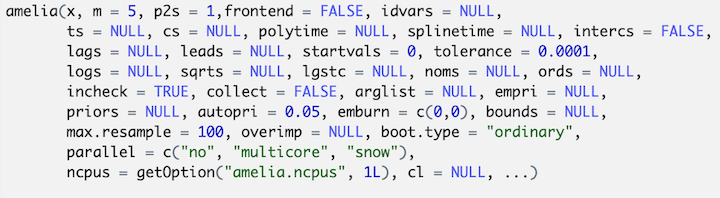
\includegraphics{figures/amelia.png}
  \caption{The \texttt{amelia} function}
  \label{amelia-func}
\end{figure}
As with \texttt{mice}, the majority of arguments are not of importance to general users. Specifications such as \texttt{splinetime}, which allows the control of cubic smoothing splines of time, and \texttt{lags}, which indicates columns in the data that should have their lags included in the imputation model, will only be used in very particular situations by a small minority of users. Other arguments likewise are not crucial to the basic workings of the function, such as \texttt{p2s} to control console printing and \texttt{parallel} to identify any type of parallel operation to be used.

The only argument that requires user input is \texttt{x}, which needs to be data with missing values that can be in a variety of formats. \texttt{m}, identical to \texttt{mice}, should be adjusted to reflect the percentage of missingness in the data. Three other arguments are important since they arguably comprise the core of \texttt{amelia}'s underlying imputation mechanism: \texttt{tolerance}, \texttt{autopri}, and \texttt{boot.type}. \texttt{tolerance} sets the convergence threshold for the EM algorithm. \texttt{autopri} allows the EM chain to increase the empirical prior if the path strays into an non-positive definite covariance matrix. \texttt{boot.type} offers the option to turn off the non-parametric bootstrap that is applied by default.

General multiple imputation research treats independent ordinal variables as continuous variables. \texttt{amelia} supports this and treats ordinal variables as continuous variables as a default. This means missing ordinal variables are imputed on a continuous scale, rather than preserved as the factual levels present in the observed data. However, the \texttt{ords} argument allows users to `disable' continuous ordinal imputation. In this case, ordinal variables are still imputed on a continuous scale, but these imputations are then scaled and used as the probability of success in a binomial distribution. The draw from this binomial distribution is then transformed into one of the ordinal levels present in the observed data by rounding. While \texttt{amelia} thus does incorporate ordinal variables to some extent, the rounding process changes the nature of ordinal variables to continuous variables. In addition, none of its features address or reflect the spacing between the ordinal variable categories.

\hypertarget{ordmiss-theory-multimpute-hdnorm}{%
\subsubsection{\texorpdfstring{\texttt{hot.deck}: Multiple Hot Deck Imputation}{hot.deck: Multiple Hot Deck Imputation}}\label{ordmiss-theory-multimpute-hdnorm}}

\texttt{hot.deck} is an \texttt{R} package released in 2012 (Gill \& Cranmer, 2012). It combines a variation of non-parametric hot decking (see section \ref{ordmiss-theory-singimpute}) with multiple imputation and aims to fill gaps where parametric multiple imputation, i.e.~the approach used in \texttt{mice} and \texttt{amelia}, falls short (Fuller \& Kim, 2005; Kim, 2004; Kim \& Fuller, 2004; Reilly, 1993). Like hot decking, \texttt{hot.deck} uses draws of actual observable values (\textit{donors}) to fill missing values (\textit{recipients}). In order to account for uncertainty around the drawn values, \texttt{hot.deck} iterates these draws over \(m\) imputations and pools the results.

The main proposed advantage of \texttt{hot.deck} lies in its applicability to missing data with discrete variables with a small number of categories. Approaches like the one used in \texttt{amelia}, for instance, by default impute discrete data on a continuous scale. This changes the nature of discrete variables and practically turns them into continuous variables. This can result in non-observable, biased, and sometimes even non-sensical imputation values with artificially smaller standard errors. The proposed \texttt{amelia} solution of rounding continuous imputations is problematic as well: Let imputation 1 of a binary variable between 0 and 1 be 0.4. Let further imputation 2 of the binary variable be 0.6. With rounding, these imputations become 0 and 1, when they are in fact 0.4 and 0.6. Rounding thus by definition introduces at least some level of bias. The problem is exacerbated for ordinal variables, where the spacing between the discrete variable categories is unknown, since it arbitrarily reduces or lengthens distances between the categories. This is not the case in \texttt{hot.deck} as it preserves the integrity of discrete data, does not change the size of standard errors, and produces more accurate imputations. \texttt{hot.deck} also does not require assumptions of a MVN distribution that are required by \texttt{amelia}.

Following Gill \& Cranmer (2012), \texttt{hot.deck} estimates affinity scores, \(\alpha\), for each missing value to measure how similar a respondent with a missing value, the recipient \(c\), is to another respondent, the potential donor \(o\), across all variables except the missing one. Each score is bounded by 0 and 1. The total set of affinity scores is denoted by \(\alpha_{co}\). For each respondent, let there be vector \((p, v)\), with \(p\) being the dependent variable and \(v\) a vector of discrete explanatory variables of length \(k\). If recipient \(c\) has \(q_c\) missing values in \(v_c\), then the potential donor vector, \(v_o\) has between 0 and \(k-q_c\) exact matches with \(c\). Let \(w_{co}\) be the number of variables where \(c\) and \(o\) have non-identical values. This leaves \(k-q_c -w_{co}\) as the number of variables where they have identical values. Scaled by the highest number of possible matches \((k-q_c)\), this value forms the affinity score
\begin{align}
\alpha_{co} = \frac{k-q_c-w_{co}}{k-q_c}
\end{align}
for each missing value recipient \(c\). When the number of identical matches decreases, so does \(\alpha_{co}\). While this might work well for binary variables, it poses a problem for discrete variables with many levels, as the probability to find identical matches decreases. To account for this, \texttt{hot.deck} treats potential donors \(o\) for the \(h\)th variable in \(v_{o[h]}\) that are `close' differently than potential donors \(o\) that are further away. `Close' is defined as \(v_{o[h]}\) and \(v_{c[h]}\) being in the same concentric standard deviation from \(\overline{h}\), the mean of variable \(h\). Values outside of this range are penalized while values within this range are counted as matches. All donors with the highest affinity scores, i.e.~all matches, form the best imputation cell \(B\). Since all values of \(v_{c[h]}\) in \(B\) are part of the same distribution of independent and identically distributed (iid) random variables, which satisfies the MCAR requirement, we can use random draws from \(B\) to impute the missing value. As with the other multiple imputation approaches, this process is then repeated \(m\) times for each missing value to account for imputation uncertainty, following the logic displayed in Figure \ref{mi-workflow}.

Figure \ref{hot.deck-func} shows the package's main imputation function, \texttt{hot.deck}, with all its arguments. As before, I will use \texttt{hot.deck} with its default settings.
\begin{figure}[hbt]
  \centering
  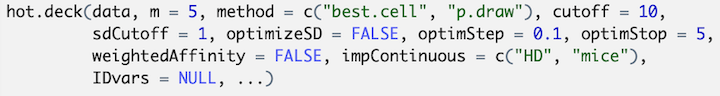
\includegraphics{figures/hot.deck.png}
  \caption{The \texttt{hot.deck} function}
  \label{hot.deck-func}
\end{figure}
Like \texttt{mice} and \texttt{amelia}, \texttt{hot.deck} only requires user input for \texttt{data}. \texttt{m} should once more be set to the percentage of missingness. Specialized arguments such as \texttt{optimStep} and \texttt{optimStop}, which can be tweaked to optimize standard deviation cutoff parameters, as well as \texttt{weightedAffinity}, which indicates whether a correlation-weighted affinity score should be used, do not apply to general users.

\texttt{method} and \texttt{cutoff} form the core of \texttt{hot.deck}. The default setting of \texttt{best.cell} in the \texttt{method} argument implements multiple hot deck imputation. The alternative, \texttt{p.draw}, on the other hand, merely conducts random probabilistic draws. \texttt{cutoff} allows users to specify which variables the algorithm should treat as discrete. By default, any variable up to and including ten unique values is considered discrete. This thus includes the majority of political science survey measures, with the sensible exceptions of variables like age or for instance widely spread assessments of income levels.

Overall, \texttt{hot.deck} is a specialized function to improve the application of multiple imputation for discrete data and has been shown to do so for highly granular discrete data (Gill \& Cranmer, 2012). Moreover, political science survey research relies on highly discrete measures. What is missing from \texttt{hot.deck}, however, is the incorporation of ordinal variables as a special form of discrete data. I thus identify this gap as the ideal leverage point to improve the use of ordinal variables in the imputation of missing data. To do so, I adapt \texttt{hot.deck} to form \texttt{hd.ord}, a function specifically designed to utilize the ordered but unevenly spaced information contained in ordinal variables.

\hypertarget{ordmiss-theory-multimpute-hdord}{%
\subsubsection{\texorpdfstring{\texttt{hd.ord}: Multiple Hot Deck Imputation with Ordinal Variables}{hd.ord: Multiple Hot Deck Imputation with Ordinal Variables}}\label{ordmiss-theory-multimpute-hdord}}

\texttt{hd.ord} is a self-penned \texttt{R} function designed specifically to implement multiple hot deck imputation with ordinal variables. It is an extension of \texttt{hot.deck} and fully utilizes the unevenly spaced yet ordered information contained in ordinal variables. As described in section \ref{intro-ordinal}, ordinal variables matter in political science surveys because a key variable in such surveys is ordinal: Education. The importance of the spacing between education values is best demonstrated with a simplified example shown in Table \ref{ordmiss-ordspace}.
\begin{table}[ht]
  \centering
  \begin{tabular}{lccccc}
  \bottomrule 
  \midrule
  Respondent & Age & Party ID & Education & Income & Gender\\
  \hline
  A & 25 & Republican & High School Graduate & \$30-40,000 & Male \\
  B & 40 & NA & Some High School &  \$20-30,000 & Female\\
  C & 30 & Democrat & Bachelor's Degree &  \$50-60,000 & Female\\
  \bottomrule 
  \end{tabular}
  \caption{Illustrative Data}.
  \label{ordmiss-ordspace}
\end{table}
Respondent B shows missing data for party ID. To impute a fill-in value, we look at how close respondents A and C are to B in terms of age, education, income, and gender. C is closer to B in terms of age and they share the same gender. A is closer to B on education and income. \texttt{hot.deck} measures these distances and estimates affinity scores for respondents A and C. The affinity scores measure how close A and C are to B on all variables except the missing one, i.e.~party ID. B then receives the party ID fill-in value from whichever respondent has the higher score. The algorithm building the affinity score is based on evenly spaced sequential numeric values, e.g.~1, 2, 3 etc. to represent the distances between the variable categories. This makes sense for age, income, and gender, but not for education, since education is an ordinal variable. Applying \texttt{hot.deck} to such a numeric representation would misrepresent the data.

Instead, \texttt{hd.ord} applies \texttt{polr} from the \texttt{MASS} package to any specified number of ordinal variables in the data to estimate the underlying latent continuous variable. This estimates cutoff thresholds between the ordinal categories and bins data cases according to the linear predictors. The binned cases determine which variable categories make sense, given the underlying latent continuous variable. This can result in a reduction of education categories if the categories are too finely thinned out. \texttt{hd.ord} uses these newly estimated categories. Rather than following the convention of assigning evenly spaced sequential numeric values to them, the function estimates the mid-cutpoints between each category, based on the \texttt{polr} results. We then replace the ordinal variable categories with the newly estimated numeric mid-cutpoints in the data. Finally, these values are scaled and used in the assessment of distance to calculate affinity scores.

Table \ref{ordmiss-ill-res} displays illustrative results from running \texttt{polr} on survey data, with column ``Thresholds'' showing the estimated cutoff thresholds between the education categories. Table \ref{ordmiss-ill-mid} in turn shows the estimated mid-cutpoints for each of the education categories. The mid-cutpoint values for the categories in Table \ref{ordmiss-ill-mid} fall between the adjacent values in Table \ref{ordmiss-ill-res}, i.e.~the mid-cutpoint of .547 for Some High School lies between the respective thresholds of .032 and 1.063. To estimate the beginning cutpoint for the first category (Less Than High School), we halve the difference between the first and second threshold and subtract this value from the first threshold: .032 \(-\) (1.063 \(-\) 0.032) / 2 = -0.483. The same process is applied to estimate the ending cutpoint for the last category (Master's Degree). The mid-cutpoint values are then scaled and used for the calculation of the affinity scores.
\begin{table}[!htbp] \centering 
  \caption{Illustrative Data polr Results} 
  \label{ordmiss-ill-res} 
\begin{tabular}{@{\extracolsep{5pt}} D{.}{.}{-3} D{.}{.}{-3} } 
\\[-1.8ex]\hline 
\hline \\[-1.8ex] 
\multicolumn{1}{c}{Intercepts} & \multicolumn{1}{c}{Thresholds} \\ 
\hline \\[-1.8ex] 
\multicolumn{1}{c}{Less Than High School\textbar Some High School} & \multicolumn{1}{c}{.032} \\ 
\multicolumn{1}{c}{Some High School\textbar High School Graduate} & \multicolumn{1}{c}{1.063} \\ 
\multicolumn{1}{c}{High School Graduate\textbar Some College} & \multicolumn{1}{c}{1.783} \\ 
\multicolumn{1}{c}{Some College\textbar Bachelor's Degree} & \multicolumn{1}{c}{3.302} \\ 
\multicolumn{1}{c}{Bachelor's Degree\textbar Master's Degree} & \multicolumn{1}{c}{4.907} \\ 
\hline \\[-1.8ex] 
\end{tabular} 
\end{table}
\begin{table}[!htbp] \centering 
  \caption{Illustrative Data Value Replacements} 
  \label{ordmiss-ill-mid} 
\begin{tabular}{@{\extracolsep{5pt}} D{.}{.}{-3} D{.}{.}{-3} } 
\\[-1.8ex]\hline 
\hline \\[-1.8ex] 
\multicolumn{1}{c}{Original Education Categories} & \multicolumn{1}{c}{Mid-Cutpoints} \\ 
\hline \\[-1.8ex] 
\multicolumn{1}{c}{Less Than High School} & \multicolumn{1}{c}{-.484} \\ 
\multicolumn{1}{c}{Some High School} & \multicolumn{1}{c}{.547} \\ 
\multicolumn{1}{c}{High School Graduate} & \multicolumn{1}{c}{1.423} \\ 
\multicolumn{1}{c}{Some College} & \multicolumn{1}{c}{2.542} \\ 
\multicolumn{1}{c}{Bachelor's Degree} & \multicolumn{1}{c}{4.104} \\ 
\multicolumn{1}{c}{Master's Degree} & \multicolumn{1}{c}{5.709} \\ 
\hline \\[-1.8ex] 
\end{tabular} 
\end{table}
Figure \ref{hd.ord-func} shows my self-penned imputation function, \texttt{hd.ord}, with all its arguments. As before, I will use \texttt{hd.ord} with its default settings. Since \texttt{hd.ord} is an adaptation of \texttt{hot.deck}, the two functions are identical except for the \texttt{ord} argument, which allows users to specify the ordinal variables for \texttt{polr} treatment.
\begin{figure}[hbt]
  \centering
  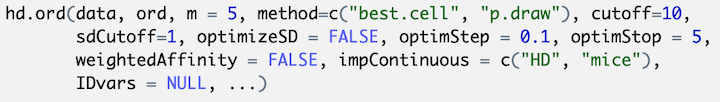
\includegraphics{figures/hd.ord.png}
  \caption{The \texttt{hd.ord} function}
  \label{hd.ord-func}
\end{figure}
\hypertarget{ordmiss-data}{%
\section{Data}\label{ordmiss-data}}

To test the performance of imputation methods, we need to work with complete data, as only complete data allow us to obtain the true values needed as a benchmark for comparison. I choose two different sets of survey data: Data from the 2016 ANES and the 2016 CCES. Data for all selected variables in both datasets is complete. In order to test the accuracy of several imputation methods, I delete data from these complete data sets with the \texttt{ampute} function from the \texttt{mice} package (Buuren et al., 2020). \texttt{ampute} allows the removal of data MCAR, MAR, and MNAR. Particularly the availability of the latter offers unique opportunities: Establishing whether real-life missing data is MNAR is a difficult feat. Data that are artificially created to be MNAR, however, circumvent this problem and allow us to test the accuracy of imputation methods for data MNAR as well. \texttt{ampute} has been shown to accurately remove data MCAR, MAR, and MNAR (Schouten, Lugtig, \& Vink, 2018).

Each dataset is imputed with four different functions: \texttt{amelia}, \texttt{mice}, \texttt{hot.deck}, and \texttt{hd.ord}. As outlined in section \ref{ordmiss-theory-multimpute}, all functions are used with their default settings with only two exceptions: The number of imputations is set to the percentage of missingness instead of the default five, and the console printing options are turned off.

I test each function for accuracy and speed for binary, ordinal, and interval variables in both datasets. Each dataset contains two ordinal (\texttt{Education}, \texttt{Interest}), two interval (\texttt{Age}, \texttt{Income}) and numerous binary variables. In order to enable factually accurate comparison and unless explicitly specified otherwise, each dataset contains 1,000 observations and six levels of the ordinal variable \texttt{Education}. 1,000 observations represent a common size for survey and survey experiment data, and the \texttt{polr} analysis from section \ref{ordblock-data} estimates five or six levels to best represent \texttt{Education} in a US context. Each dataset was imputed 1,000 times with each of the four imputation methods. With the exception of Table \ref{run.cces.perc}, 20 percent NA were randomly amputed in each iteration for each dataset.

Following Collins et al. (2001) and Honaker \& King (2010), as many relevant predictor variables as possible were used to impute each of the datasets. For the ANES data, up to 14 predictor variables were used: \texttt{Ind} (Independent), \texttt{Moderate}, \texttt{Black}, \texttt{Hisp} (Hispanic), \texttt{Asian}, \texttt{Empl} (Employed), \texttt{Stud} (Student), \texttt{Religious}, \texttt{InternetHome}, \texttt{OwnHome}, \texttt{Rally} (have you attended a political rally), \texttt{Donate} (have you donated to a political candidate), \texttt{Married}, and \texttt{Separated}. For the CCES data, up to 17 predictor variables were used: \texttt{Rep} (Republican), \texttt{Moderate}, \texttt{Liberal}, \texttt{Black}, \texttt{Hisp}, \texttt{Asian}, \texttt{Empl}, \texttt{Unempl} (Unemployed), \texttt{Stud}, \texttt{Gay}, \texttt{Bisexual}, \texttt{StudLoans} (do you have student loans), \texttt{InternetHome}, \texttt{NotReligious}, \texttt{RentHome}, \texttt{Separated}, and \texttt{Single}. Highly collinear variables were excluded with a cutoff of .6.

The variable mean serves as the baseline of comparison for the performance of each imputation method. Since each dataset is complete, we know the true variable mean of all variables. The closer a method comes to the true mean, the better its performance. Sections \ref{ordmiss-results-mar} to \ref{ordmiss-results-increaseNA} show the results in terms of performance accuracy. First, I impute both datasets MAR (section \ref{ordmiss-results-mar}) and MNAR (section \ref{ordmiss-results-mnar}) for five and 12 amputed variables. The five amputed variables are consistent across both datasets: \texttt{Democrat} (binary), \texttt{Male} (binary), \texttt{Interest} (ordinal, scaled from 1 to 4), \texttt{Income} (interval), and \texttt{Age} (interval). The 12 amputed variables contain additional variables that differ between each dataset due to availability in the data. I do not impute these datasets MCAR for obvious reasons: Imputation is not necessary for data MCAR because simple deletion leads to unbiased and therefore valid results. In section \ref{ordmiss-results-increaseOrd}, I increase the number of ordinal variables to be treated by \texttt{polr} in \texttt{hd.ord} by including \texttt{Interest}. Imputations are again conducted MAR and MNAR for four and 11 amputed variables. The variables are the same as in sections \ref{ordmiss-results-mar} and \ref{ordmiss-results-mnar}, but without including \texttt{Interest}. Finally, I increase the amount of missing data to 50 percent (section \ref{ordmiss-results-increaseNA}).

Section \ref{ordmiss-results-speed} shows the results in terms of performance speed by the number of imputed variables (Table \ref{runtimes5var12var}) and the percentage of missingness (Table \ref{run.cces.perc}). All running times were achieved on a Code Ocean AWS EC2 instance with 16 cores and 120 GB of memory.

\hypertarget{ordmiss-results}{%
\section{Results}\label{ordmiss-results}}

\hypertarget{ordmiss-results-mar}{%
\subsection{MAR}\label{ordmiss-results-mar}}

This section shows the imputation results for the MAR missing data mechanism. MAR amputation was achieved by setting the \texttt{mech} argument in the \texttt{ampute} function to \texttt{MAR}. Table \ref{mar.5var} shows the results of imputing both datasets MAR for five amputed variables. For the two binary variables, \texttt{Dem} and \texttt{Male}, \texttt{hd.ord} performs on par or worse than \texttt{hot.deck} for both datasets, while \texttt{mice} and \texttt{amelia} perform best. \texttt{hd.ord} is relatively close for CCES \texttt{Dem} (+.0001 \texttt{amelia} vs.~+.0000 \texttt{hd.ord}) but further away for ANES ( +.0003 \texttt{mice} vs.~--.0010 \texttt{hd.ord} \texttt{Dem}; +.0001 \texttt{mice} vs.~--.0013 \texttt{hd.ord} \texttt{Male}) and CCES \texttt{Male} (--.0001 \texttt{amelia} vs.~--.0011 \texttt{hd.ord}).
\begin{table}[!htbp] \centering 
  \caption{Accuracy of Multiple Imputation Methods. MAR, 5 Variables with NA} 
  \label{mar.5var} 
\begin{threeparttable}
\begin{tabular}{@{\extracolsep{5pt}} D{.}{.}{-4} D{.}{.}{-4} D{.}{.}{-4} D{.}{.}{-4} } 
\\[-1.8ex]\hline 
\hline \\[-1.8ex] 
\multicolumn{1}{c}{Method} & \multicolumn{1}{c}{Variable} & \multicolumn{1}{c}{ANES} & \multicolumn{1}{c}{CCES} \\ 
\hline \\[-1.8ex] 
\multicolumn{1}{c}{true} & \multicolumn{1}{c}{Dem} & \multicolumn{1}{c}{.3420} & \multicolumn{1}{c}{.3770} \\ 
\multicolumn{1}{c}{hd.ord} & \multicolumn{1}{c}{Dem} & \multicolumn{1}{c}{--.0010} & \multicolumn{1}{c}{+.0000} \\ 
\multicolumn{1}{c}{hot.deck} & \multicolumn{1}{c}{Dem} & \multicolumn{1}{c}{--.0011} & \multicolumn{1}{c}{--.0004} \\ 
\multicolumn{1}{c}{amelia} & \multicolumn{1}{c}{Dem} & \multicolumn{1}{c}{+.0004} & \multicolumn{1}{c}{+.0001} \\ 
\multicolumn{1}{c}{mice} & \multicolumn{1}{c}{Dem} & \multicolumn{1}{c}{+.0003} & \multicolumn{1}{c}{+.0002} \\ 
\multicolumn{1}{c}{na.omit} & \multicolumn{1}{c}{Dem} & \multicolumn{1}{c}{--.0290} & \multicolumn{1}{c}{--.0229} \\ 
\multicolumn{1}{c}{true} & \multicolumn{1}{c}{Male} & \multicolumn{1}{c}{.4890} & \multicolumn{1}{c}{.4830} \\ 
\multicolumn{1}{c}{hd.ord} & \multicolumn{1}{c}{Male} & \multicolumn{1}{c}{--.0013} & \multicolumn{1}{c}{--.0011} \\ 
\multicolumn{1}{c}{hot.deck} & \multicolumn{1}{c}{Male} & \multicolumn{1}{c}{--.0013} & \multicolumn{1}{c}{--.0014} \\ 
\multicolumn{1}{c}{amelia} & \multicolumn{1}{c}{Male} & \multicolumn{1}{c}{+.0002} & \multicolumn{1}{c}{--.0001} \\ 
\multicolumn{1}{c}{mice} & \multicolumn{1}{c}{Male} & \multicolumn{1}{c}{+.0001} & \multicolumn{1}{c}{--.0001} \\ 
\multicolumn{1}{c}{na.omit} & \multicolumn{1}{c}{Male} & \multicolumn{1}{c}{--.0392} & \multicolumn{1}{c}{--.0414} \\ 
\multicolumn{1}{c}{true} & \multicolumn{1}{c}{Interest} & \multicolumn{1}{c}{2.9340} & \multicolumn{1}{c}{3.3290} \\ 
\multicolumn{1}{c}{hd.ord} & \multicolumn{1}{c}{Interest} & \multicolumn{1}{c}{--.0130} & \multicolumn{1}{c}{--.0125} \\ 
\multicolumn{1}{c}{hot.deck} & \multicolumn{1}{c}{Interest} & \multicolumn{1}{c}{--.0191} & \multicolumn{1}{c}{--.0196} \\ 
\multicolumn{1}{c}{amelia} & \multicolumn{1}{c}{Interest} & \multicolumn{1}{c}{+.0003} & \multicolumn{1}{c}{+.0003} \\ 
\multicolumn{1}{c}{mice} & \multicolumn{1}{c}{Interest} & \multicolumn{1}{c}{+.0003} & \multicolumn{1}{c}{+.0000} \\ 
\multicolumn{1}{c}{na.omit} & \multicolumn{1}{c}{Interest} & \multicolumn{1}{c}{--.0705} & \multicolumn{1}{c}{--.0724} \\ 
\multicolumn{1}{c}{true} & \multicolumn{1}{c}{Inc} & \multicolumn{1}{c}{16.6140} & \multicolumn{1}{c}{6.4810} \\ 
\multicolumn{1}{c}{hd.ord} & \multicolumn{1}{c}{Inc} & \multicolumn{1}{c}{--.1068} & \multicolumn{1}{c}{--.0259} \\ 
\multicolumn{1}{c}{hot.deck} & \multicolumn{1}{c}{Inc} & \multicolumn{1}{c}{--.1278} & \multicolumn{1}{c}{--.0407} \\ 
\multicolumn{1}{c}{amelia} & \multicolumn{1}{c}{Inc} & \multicolumn{1}{c}{+.0008} & \multicolumn{1}{c}{--.0004} \\ 
\multicolumn{1}{c}{mice} & \multicolumn{1}{c}{Inc} & \multicolumn{1}{c}{+.0003} & \multicolumn{1}{c}{--.0002} \\ 
\multicolumn{1}{c}{na.omit} & \multicolumn{1}{c}{Inc} & \multicolumn{1}{c}{--.5631} & \multicolumn{1}{c}{--.2468} \\ 
\multicolumn{1}{c}{true} & \multicolumn{1}{c}{Age} & \multicolumn{1}{c}{50.0410} & \multicolumn{1}{c}{52.8230} \\ 
\multicolumn{1}{c}{hd.ord} & \multicolumn{1}{c}{Age} & \multicolumn{1}{c}{--.3888} & \multicolumn{1}{c}{--.2616} \\ 
\multicolumn{1}{c}{hot.deck} & \multicolumn{1}{c}{Age} & \multicolumn{1}{c}{--.4597} & \multicolumn{1}{c}{--.3895} \\ 
\multicolumn{1}{c}{amelia} & \multicolumn{1}{c}{Age} & \multicolumn{1}{c}{+.0007} & \multicolumn{1}{c}{--.0033} \\ 
\multicolumn{1}{c}{mice} & \multicolumn{1}{c}{Age} & \multicolumn{1}{c}{+.0017} & \multicolumn{1}{c}{--.0073} \\ 
\multicolumn{1}{c}{na.omit} & \multicolumn{1}{c}{Age} & \multicolumn{1}{c}{--1.1875} & \multicolumn{1}{c}{--1.2361} \\ 
\hline \\[-1.8ex] 
\end{tabular} 
\begin{tablenotes}[para,flushleft]
\footnotesize{\textit{Note:} Each \texttt{true} value shows the true variable mean. All other values show the differences between the imputation means and the true mean, indicated with a + or -- sign.}
\end{tablenotes}
\end{threeparttable}
\end{table}
For the ordinal variable, \texttt{Interest}, \texttt{hd.ord} performs worst for both datasets, with considerable distance to \texttt{hot.deck} (--.0130 vs.~--.0191 ANES; --.0125 vs.~--.0196 CCES). \texttt{mice} and \texttt{amelia} perform by far best across both datasets. The performance differences between the methods are far larger for the ordinal than for the binary variables: \texttt{mice} is not more than +.0003 (ANES) away from the true value across both datasets, while the maximum difference for \texttt{hd.ord} amounts to --.0130 (ANES).

For the interval variables, \texttt{Inc} and \texttt{Age}, \texttt{hd.ord} also performs worst for both datasets. The distance to \texttt{hot.deck} is once more considerable. \texttt{mice} performs best for \texttt{Inc} and \texttt{amelia} shows the best results for \texttt{Age}. The performance differences between the methods are even larger here: For \texttt{Inc}, \texttt{mice} is not more than --.0002 (CCES) away from the true value across both datasets, but the maximum difference for \texttt{hd.ord} is --.1068 (ANES). Similarly, \texttt{amelia}'s largest deviation from the true value for \texttt{Age} is --.0033 (CCES) as opposed to \texttt{hd.ord}'s --.3888 (ANES).

Table \ref{mar.12var} shows the results of imputing both datasets MAR for 12 amputed variables. The first five listed variables are the same as for the MAR analysis for five amputed variables in Table \ref{mar.5var}. The remaining variables were chosen based on availability in each dataset. As much as possible, the same variables were selected across both datasets. \texttt{Black}, \texttt{Empl}, \texttt{Religious}, \texttt{Married}, \texttt{OwnHome}, \texttt{Rally}, \texttt{Donate}, \texttt{Gay}, \texttt{StudLoans}, \texttt{Hisp}, \texttt{Official}, and \texttt{Stud} are binary variables. \texttt{Black} indicates whether a respondent is of African-American origin, \texttt{Empl} whether she is currently employed, \texttt{Religious} whether she follows a religious belief, \texttt{Married} whether she is currently married, \texttt{OwnHome} whether she owns her home, \texttt{Rally} whether she has attended a political rally, \texttt{Donate} whether she has donated to a political candidate, \texttt{Gay} whether she identifies as homosexual, \texttt{StudLoans} whether she currently has student loans, \texttt{Hisp} whether she is of Hispanic origin, \texttt{Official} whether she has contacted her political representative, and \texttt{Stud} whether she currently is a student. \texttt{Media} is an ordinal variable and indicates how much she follows public affairs in the media (scaled from 1 to 5). \texttt{Participation} is an interval variable and shows the accumulative count of political activities she has participated in (scaled from 0 to 4).

\ssp

\footnotesize
\begin{longtable}{@{\extracolsep{5pt}} D{.}{.}{-4} D{.}{.}{-4} D{.}{.}{-4} D{.}{.}{-4} } 
  \caption{Accuracy of Multiple Imputation Methods. MAR, 12 Variables with NA} 
  \label{mar.12var} 
\\[-1.8ex]\hline 
\hline \\[-1.8ex] 
\multicolumn{1}{c}{Method} & \multicolumn{1}{c}{Variable} & \multicolumn{1}{c}{ANES} & \multicolumn{1}{c}{CCES} \\ 
\hline \\[-1.8ex] 
\multicolumn{1}{c}{true} & \multicolumn{1}{c}{Dem} & \multicolumn{1}{c}{.3420} & \multicolumn{1}{c}{.3770} \\ 
\multicolumn{1}{c}{hd.ord} & \multicolumn{1}{c}{Dem} & \multicolumn{1}{c}{--.0005} & \multicolumn{1}{c}{--.0003} \\ 
\multicolumn{1}{c}{hot.deck} & \multicolumn{1}{c}{Dem} & \multicolumn{1}{c}{--.0005} & \multicolumn{1}{c}{--.0004} \\ 
\multicolumn{1}{c}{amelia} & \multicolumn{1}{c}{Dem} & \multicolumn{1}{c}{+.0000} & \multicolumn{1}{c}{+.0000} \\ 
\multicolumn{1}{c}{mice} & \multicolumn{1}{c}{Dem} & \multicolumn{1}{c}{+.0000} & \multicolumn{1}{c}{+.0001} \\ 
\multicolumn{1}{c}{na.omit} & \multicolumn{1}{c}{Dem} & \multicolumn{1}{c}{--.0191} & \multicolumn{1}{c}{--.0172} \\ 
\multicolumn{1}{c}{true} & \multicolumn{1}{c}{Male} & \multicolumn{1}{c}{.4890} & \multicolumn{1}{c}{.4830} \\ 
\multicolumn{1}{c}{hd.ord} & \multicolumn{1}{c}{Male} & \multicolumn{1}{c}{--.0004} & \multicolumn{1}{c}{--.0002} \\ 
\multicolumn{1}{c}{hot.deck} & \multicolumn{1}{c}{Male} & \multicolumn{1}{c}{--.0001} & \multicolumn{1}{c}{--.0003} \\ 
\multicolumn{1}{c}{amelia} & \multicolumn{1}{c}{Male} & \multicolumn{1}{c}{+.0001} & \multicolumn{1}{c}{--.0001} \\ 
\multicolumn{1}{c}{mice} & \multicolumn{1}{c}{Male} & \multicolumn{1}{c}{+.0000} & \multicolumn{1}{c}{--.0002} \\ 
\multicolumn{1}{c}{na.omit} & \multicolumn{1}{c}{Male} & \multicolumn{1}{c}{--.0256} & \multicolumn{1}{c}{--.0364} \\ 
\multicolumn{1}{c}{true} & \multicolumn{1}{c}{Interest} & \multicolumn{1}{c}{2.9340} & \multicolumn{1}{c}{3.3290} \\ 
\multicolumn{1}{c}{hd.ord} & \multicolumn{1}{c}{Interest} & \multicolumn{1}{c}{--.0053} & \multicolumn{1}{c}{--.0041} \\ 
\multicolumn{1}{c}{hot.deck} & \multicolumn{1}{c}{Interest} & \multicolumn{1}{c}{--.0077} & \multicolumn{1}{c}{--.0067} \\ 
\multicolumn{1}{c}{amelia} & \multicolumn{1}{c}{Interest} & \multicolumn{1}{c}{+.0001} & \multicolumn{1}{c}{--.0001} \\ 
\multicolumn{1}{c}{mice} & \multicolumn{1}{c}{Interest} & \multicolumn{1}{c}{+.0000} & \multicolumn{1}{c}{--.0001} \\ 
\multicolumn{1}{c}{na.omit} & \multicolumn{1}{c}{Interest} & \multicolumn{1}{c}{--.0620} & \multicolumn{1}{c}{--.0515} \\ 
\multicolumn{1}{c}{true} & \multicolumn{1}{c}{Inc} & \multicolumn{1}{c}{16.6140} & \multicolumn{1}{c}{6.4810} \\ 
\multicolumn{1}{c}{hd.ord} & \multicolumn{1}{c}{Inc} & \multicolumn{1}{c}{--.0470} & \multicolumn{1}{c}{--.0130} \\ 
\multicolumn{1}{c}{hot.deck} & \multicolumn{1}{c}{Inc} & \multicolumn{1}{c}{--.0591} & \multicolumn{1}{c}{--.0212} \\ 
\multicolumn{1}{c}{amelia} & \multicolumn{1}{c}{Inc} & \multicolumn{1}{c}{--.0007} & \multicolumn{1}{c}{--.0005} \\ 
\multicolumn{1}{c}{mice} & \multicolumn{1}{c}{Inc} & \multicolumn{1}{c}{--.0013} & \multicolumn{1}{c}{--.0003} \\ 
\multicolumn{1}{c}{na.omit} & \multicolumn{1}{c}{Inc} & \multicolumn{1}{c}{--.6303} & \multicolumn{1}{c}{--.2860} \\ 
\multicolumn{1}{c}{true} & \multicolumn{1}{c}{Age} & \multicolumn{1}{c}{50.0410} & \multicolumn{1}{c}{52.8230} \\ 
\multicolumn{1}{c}{hd.ord} & \multicolumn{1}{c}{Age} & \multicolumn{1}{c}{--.1391} & \multicolumn{1}{c}{--.0883} \\ 
\multicolumn{1}{c}{hot.deck} & \multicolumn{1}{c}{Age} & \multicolumn{1}{c}{--.1835} & \multicolumn{1}{c}{--.1435} \\ 
\multicolumn{1}{c}{amelia} & \multicolumn{1}{c}{Age} & \multicolumn{1}{c}{+.0056} & \multicolumn{1}{c}{--.0015} \\ 
\multicolumn{1}{c}{mice} & \multicolumn{1}{c}{Age} & \multicolumn{1}{c}{+.0048} & \multicolumn{1}{c}{--.0050} \\ 
\multicolumn{1}{c}{na.omit} & \multicolumn{1}{c}{Age} & \multicolumn{1}{c}{--.8638} & \multicolumn{1}{c}{--.5974} \\ 
\multicolumn{1}{c}{true} & \multicolumn{1}{c}{Black} & \multicolumn{1}{c}{.0790} & \multicolumn{1}{c}{.0950} \\ 
\multicolumn{1}{c}{hd.ord} & \multicolumn{1}{c}{Black} & \multicolumn{1}{c}{+.0000} & \multicolumn{1}{c}{+.0000} \\ 
\multicolumn{1}{c}{hot.deck} & \multicolumn{1}{c}{Black} & \multicolumn{1}{c}{+.0000} & \multicolumn{1}{c}{+.0000} \\ 
\multicolumn{1}{c}{amelia} & \multicolumn{1}{c}{Black} & \multicolumn{1}{c}{+.0000} & \multicolumn{1}{c}{+.0001} \\ 
\multicolumn{1}{c}{mice} & \multicolumn{1}{c}{Black} & \multicolumn{1}{c}{+.0000} & \multicolumn{1}{c}{+.0001} \\ 
\multicolumn{1}{c}{na.omit} & \multicolumn{1}{c}{Black} & \multicolumn{1}{c}{--.0092} & \multicolumn{1}{c}{--.0090} \\ 
\multicolumn{1}{c}{true} & \multicolumn{1}{c}{Empl} & \multicolumn{1}{c}{.6610} & \multicolumn{1}{c}{.4370} \\ 
\multicolumn{1}{c}{hd.ord} & \multicolumn{1}{c}{Empl} & \multicolumn{1}{c}{+.0006} & \multicolumn{1}{c}{+.0000} \\ 
\multicolumn{1}{c}{hot.deck} & \multicolumn{1}{c}{Empl} & \multicolumn{1}{c}{+.0006} & \multicolumn{1}{c}{+.0001} \\ 
\multicolumn{1}{c}{amelia} & \multicolumn{1}{c}{Empl} & \multicolumn{1}{c}{+.0000} & \multicolumn{1}{c}{+.0000} \\ 
\multicolumn{1}{c}{mice} & \multicolumn{1}{c}{Empl} & \multicolumn{1}{c}{+.0000} & \multicolumn{1}{c}{--.0001} \\ 
\multicolumn{1}{c}{na.omit} & \multicolumn{1}{c}{Empl} & \multicolumn{1}{c}{--.0087} & \multicolumn{1}{c}{--.0301} \\ 
\multicolumn{1}{c}{true} & \multicolumn{1}{c}{Religious} & \multicolumn{1}{c}{.6460} & \multicolumn{1}{c}{.6420} \\ 
\multicolumn{1}{c}{hd.ord} & \multicolumn{1}{c}{Religious} & \multicolumn{1}{c}{--.0006} & \multicolumn{1}{c}{--.0003} \\ 
\multicolumn{1}{c}{hot.deck} & \multicolumn{1}{c}{Religious} & \multicolumn{1}{c}{--.0005} & \multicolumn{1}{c}{--.0003} \\ 
\multicolumn{1}{c}{amelia} & \multicolumn{1}{c}{Religious} & \multicolumn{1}{c}{--.0001} & \multicolumn{1}{c}{--.0001} \\ 
\multicolumn{1}{c}{mice} & \multicolumn{1}{c}{Religious} & \multicolumn{1}{c}{--.0001} & \multicolumn{1}{c}{--.0002} \\ 
\multicolumn{1}{c}{na.omit} & \multicolumn{1}{c}{Religious} & \multicolumn{1}{c}{--.0166} & \multicolumn{1}{c}{--.0234} \\ 
\multicolumn{1}{c}{true} & \multicolumn{1}{c}{Married} & \multicolumn{1}{c}{.5290} & \multicolumn{1}{c}{.6310} \\ 
\multicolumn{1}{c}{hd.ord} & \multicolumn{1}{c}{Married} & \multicolumn{1}{c}{+.0002} & \multicolumn{1}{c}{--.0001} \\ 
\multicolumn{1}{c}{hot.deck} & \multicolumn{1}{c}{Married} & \multicolumn{1}{c}{+.0002} & \multicolumn{1}{c}{+.0001} \\ 
\multicolumn{1}{c}{amelia} & \multicolumn{1}{c}{Married} & \multicolumn{1}{c}{--.0001} & \multicolumn{1}{c}{--.0002} \\ 
\multicolumn{1}{c}{mice} & \multicolumn{1}{c}{Married} & \multicolumn{1}{c}{--.0001} & \multicolumn{1}{c}{--.0002} \\ 
\multicolumn{1}{c}{na.omit} & \multicolumn{1}{c}{Married} & \multicolumn{1}{c}{--.0384} & \multicolumn{1}{c}{--.0326} \\ 
\multicolumn{1}{c}{true} & \multicolumn{1}{c}{OwnHome} & \multicolumn{1}{c}{.6820} & \multicolumn{1}{c}{.7010} \\ 
\multicolumn{1}{c}{hd.ord} & \multicolumn{1}{c}{OwnHome} & \multicolumn{1}{c}{--.0001} & \multicolumn{1}{c}{--.0002} \\ 
\multicolumn{1}{c}{hot.deck} & \multicolumn{1}{c}{OwnHome} & \multicolumn{1}{c}{+.0000} & \multicolumn{1}{c}{+.0000} \\ 
\multicolumn{1}{c}{amelia} & \multicolumn{1}{c}{OwnHome} & \multicolumn{1}{c}{+.0001} & \multicolumn{1}{c}{+.0000} \\ 
\multicolumn{1}{c}{mice} & \multicolumn{1}{c}{OwnHome} & \multicolumn{1}{c}{--.0001} & \multicolumn{1}{c}{--.0001} \\ 
\multicolumn{1}{c}{na.omit} & \multicolumn{1}{c}{OwnHome} & \multicolumn{1}{c}{--.0334} & \multicolumn{1}{c}{--.0304} \\ 
\multicolumn{1}{c}{true} & \multicolumn{1}{c}{Rally} & \multicolumn{1}{c}{.0830} & \multicolumn{1}{c}{---} \\ 
\multicolumn{1}{c}{hd.ord} & \multicolumn{1}{c}{Rally} & \multicolumn{1}{c}{--.0001} & \multicolumn{1}{c}{---} \\ 
\multicolumn{1}{c}{hot.deck} & \multicolumn{1}{c}{Rally} & \multicolumn{1}{c}{--.0002} & \multicolumn{1}{c}{---} \\ 
\multicolumn{1}{c}{amelia} & \multicolumn{1}{c}{Rally} & \multicolumn{1}{c}{+.0001} & \multicolumn{1}{c}{---} \\ 
\multicolumn{1}{c}{mice} & \multicolumn{1}{c}{Rally} & \multicolumn{1}{c}{+.0001} & \multicolumn{1}{c}{---} \\ 
\multicolumn{1}{c}{na.omit} & \multicolumn{1}{c}{Rally} & \multicolumn{1}{c}{--.0191} & \multicolumn{1}{c}{---} \\ 
\multicolumn{1}{c}{true} & \multicolumn{1}{c}{Donate} & \multicolumn{1}{c}{.1390} & \multicolumn{1}{c}{---} \\ 
\multicolumn{1}{c}{hd.ord} & \multicolumn{1}{c}{Donate} & \multicolumn{1}{c}{--.0002} & \multicolumn{1}{c}{---} \\ 
\multicolumn{1}{c}{hot.deck} & \multicolumn{1}{c}{Donate} & \multicolumn{1}{c}{--.0005} & \multicolumn{1}{c}{---} \\ 
\multicolumn{1}{c}{amelia} & \multicolumn{1}{c}{Donate} & \multicolumn{1}{c}{+.0000} & \multicolumn{1}{c}{---} \\ 
\multicolumn{1}{c}{mice} & \multicolumn{1}{c}{Donate} & \multicolumn{1}{c}{+.0001} & \multicolumn{1}{c}{---} \\ 
\multicolumn{1}{c}{na.omit} & \multicolumn{1}{c}{Donate} & \multicolumn{1}{c}{--.0320} & \multicolumn{1}{c}{---} \\ 
\multicolumn{1}{c}{true} & \multicolumn{1}{c}{Gay} & \multicolumn{1}{c}{---} & \multicolumn{1}{c}{.0420} \\ 
\multicolumn{1}{c}{hd.ord} & \multicolumn{1}{c}{Gay} & \multicolumn{1}{c}{---} & \multicolumn{1}{c}{+.0001} \\ 
\multicolumn{1}{c}{hot.deck} & \multicolumn{1}{c}{Gay} & \multicolumn{1}{c}{---} & \multicolumn{1}{c}{+.0000} \\ 
\multicolumn{1}{c}{amelia} & \multicolumn{1}{c}{Gay} & \multicolumn{1}{c}{---} & \multicolumn{1}{c}{+.0000} \\ 
\multicolumn{1}{c}{mice} & \multicolumn{1}{c}{Gay} & \multicolumn{1}{c}{---} & \multicolumn{1}{c}{+.0000} \\ 
\multicolumn{1}{c}{na.omit} & \multicolumn{1}{c}{Gay} & \multicolumn{1}{c}{---} & \multicolumn{1}{c}{--.0112} \\ 
\multicolumn{1}{c}{true} & \multicolumn{1}{c}{StudLoans} & \multicolumn{1}{c}{---} & \multicolumn{1}{c}{.1910} \\ 
\multicolumn{1}{c}{hd.ord} & \multicolumn{1}{c}{StudLoans} & \multicolumn{1}{c}{---} & \multicolumn{1}{c}{+.0003} \\ 
\multicolumn{1}{c}{hot.deck} & \multicolumn{1}{c}{StudLoans} & \multicolumn{1}{c}{---} & \multicolumn{1}{c}{+.0002} \\ 
\multicolumn{1}{c}{amelia} & \multicolumn{1}{c}{StudLoans} & \multicolumn{1}{c}{---} & \multicolumn{1}{c}{+.0000} \\ 
\multicolumn{1}{c}{mice} & \multicolumn{1}{c}{StudLoans} & \multicolumn{1}{c}{---} & \multicolumn{1}{c}{--.0001} \\ 
\multicolumn{1}{c}{na.omit} & \multicolumn{1}{c}{StudLoans} & \multicolumn{1}{c}{---} & \multicolumn{1}{c}{--.0117} \\ 
\hline \\[-1.8ex] 
\end{longtable}
\dsp

\normalsize

The results are consistent with those presented in Table \ref{mar.5var}. For the binary variables, \texttt{amelia} and \texttt{mice} again perform best with results actually matching the true variable values, though \texttt{hd.ord} arguably shows closer results than in Table \ref{mar.5var} with a maximum difference to a true value of +.0006 (ANES \texttt{Empl}). For the ordinal variable, \texttt{hd.ord} continues to perform worst across both datasets. \texttt{mice} and \texttt{amelia} again show the best results. Note, however, that \texttt{hd.ord} is less worse in terms of performance differences when compared to the MAR analysis of five imputed variables. The maximum difference to the true \texttt{Interest} value is --.0053 (ANES) for 12 variables but --.0130 (ANES) for five variables. This is possibly explained by a thinner spread of missing values across a higher number of variables, resulting in a lower number of NAs in each amputed variable.

The results for the interval variables follow the same pattern: \texttt{hd.ord} displays the worst results for both datasets. The difference to \texttt{hot.deck} is still present though less pronounced than in the MAR analysis of five imputed variables. \texttt{mice} overall performs better than \texttt{amelia} for \texttt{Inc} and \texttt{Age}, with the exceptions of ANES \texttt{Inc} (--.0007 vs.~--.0013) and CCES \texttt{Age} (--.0015 vs.~--.0050).

\hypertarget{ordmiss-results-mnar}{%
\subsection{MNAR}\label{ordmiss-results-mnar}}

This section shows the imputation results for the MNAR missing data mechanism. MNAR amputation was achieved by setting the \texttt{mech} argument in the \texttt{ampute} function to \texttt{MNAR}. All MAR and MNAR analyses are otherwise identical. Table \ref{mnar.5var} shows the results of imputing both datasets MNAR for five amputed variables. It is immediately noticeable that the differences between the methods' imputation results and the true values are much higher for all methods for all variables for both datasets. The results for \texttt{Dem} and \texttt{Male}, for instance, hover around .0100 and .0125 for both datasets. In the corresponding MAR analysis, however, the results for \texttt{Dem} and \texttt{Male} showed around .0005.
\begin{table}[!htbp] \centering 
  \caption{Accuracy of Multiple Imputation Methods. MNAR, 5 Variables with NA} 
  \label{mnar.5var} 
\begin{threeparttable}
\begin{tabular}{@{\extracolsep{5pt}} D{.}{.}{-4} D{.}{.}{-4} D{.}{.}{-4} D{.}{.}{-4} } 
\\[-1.8ex]\hline 
\hline \\[-1.8ex] 
\multicolumn{1}{c}{Method} & \multicolumn{1}{c}{Variable} & \multicolumn{1}{c}{ANES} & \multicolumn{1}{c}{CCES} \\ 
\hline \\[-1.8ex] 
\multicolumn{1}{c}{true} & \multicolumn{1}{c}{Dem} & \multicolumn{1}{c}{.3420} & \multicolumn{1}{c}{.3770} \\ 
\multicolumn{1}{c}{hd.ord} & \multicolumn{1}{c}{Dem} & \multicolumn{1}{c}{--.0114} & \multicolumn{1}{c}{--.0099} \\ 
\multicolumn{1}{c}{hot.deck} & \multicolumn{1}{c}{Dem} & \multicolumn{1}{c}{--.0120} & \multicolumn{1}{c}{--.0105} \\ 
\multicolumn{1}{c}{amelia} & \multicolumn{1}{c}{Dem} & \multicolumn{1}{c}{--.0106} & \multicolumn{1}{c}{--.0102} \\ 
\multicolumn{1}{c}{mice} & \multicolumn{1}{c}{Dem} & \multicolumn{1}{c}{--.0099} & \multicolumn{1}{c}{--.0101} \\ 
\multicolumn{1}{c}{na.omit} & \multicolumn{1}{c}{Dem} & \multicolumn{1}{c}{--.0176} & \multicolumn{1}{c}{--.0140} \\ 
\multicolumn{1}{c}{true} & \multicolumn{1}{c}{Male} & \multicolumn{1}{c}{.4890} & \multicolumn{1}{c}{.4830} \\ 
\multicolumn{1}{c}{hd.ord} & \multicolumn{1}{c}{Male} & \multicolumn{1}{c}{--.0136} & \multicolumn{1}{c}{--.0116} \\ 
\multicolumn{1}{c}{hot.deck} & \multicolumn{1}{c}{Male} & \multicolumn{1}{c}{--.0133} & \multicolumn{1}{c}{--.0124} \\ 
\multicolumn{1}{c}{amelia} & \multicolumn{1}{c}{Male} & \multicolumn{1}{c}{--.0132} & \multicolumn{1}{c}{--.0121} \\ 
\multicolumn{1}{c}{mice} & \multicolumn{1}{c}{Male} & \multicolumn{1}{c}{--.0132} & \multicolumn{1}{c}{--.0120} \\ 
\multicolumn{1}{c}{na.omit} & \multicolumn{1}{c}{Male} & \multicolumn{1}{c}{--.0214} & \multicolumn{1}{c}{--.0219} \\ 
\multicolumn{1}{c}{true} & \multicolumn{1}{c}{Interest} & \multicolumn{1}{c}{2.9340} & \multicolumn{1}{c}{3.3290} \\ 
\multicolumn{1}{c}{hd.ord} & \multicolumn{1}{c}{Interest} & \multicolumn{1}{c}{--.0288} & \multicolumn{1}{c}{--.0246} \\ 
\multicolumn{1}{c}{hot.deck} & \multicolumn{1}{c}{Interest} & \multicolumn{1}{c}{--.0335} & \multicolumn{1}{c}{--.0296} \\ 
\multicolumn{1}{c}{amelia} & \multicolumn{1}{c}{Interest} & \multicolumn{1}{c}{--.0167} & \multicolumn{1}{c}{--.0146} \\ 
\multicolumn{1}{c}{mice} & \multicolumn{1}{c}{Interest} & \multicolumn{1}{c}{--.0167} & \multicolumn{1}{c}{--.0146} \\ 
\multicolumn{1}{c}{na.omit} & \multicolumn{1}{c}{Interest} & \multicolumn{1}{c}{--.0379} & \multicolumn{1}{c}{--.0372} \\ 
\multicolumn{1}{c}{true} & \multicolumn{1}{c}{Inc} & \multicolumn{1}{c}{16.6140} & \multicolumn{1}{c}{6.4810} \\ 
\multicolumn{1}{c}{hd.ord} & \multicolumn{1}{c}{Inc} & \multicolumn{1}{c}{--.2299} & \multicolumn{1}{c}{--.0928} \\ 
\multicolumn{1}{c}{hot.deck} & \multicolumn{1}{c}{Inc} & \multicolumn{1}{c}{--.2554} & \multicolumn{1}{c}{--.1038} \\ 
\multicolumn{1}{c}{amelia} & \multicolumn{1}{c}{Inc} & \multicolumn{1}{c}{--.1225} & \multicolumn{1}{c}{--.0578} \\ 
\multicolumn{1}{c}{mice} & \multicolumn{1}{c}{Inc} & \multicolumn{1}{c}{--.1229} & \multicolumn{1}{c}{--.0566} \\ 
\multicolumn{1}{c}{na.omit} & \multicolumn{1}{c}{Inc} & \multicolumn{1}{c}{--.2770} & \multicolumn{1}{c}{--.1334} \\ 
\multicolumn{1}{c}{true} & \multicolumn{1}{c}{Age} & \multicolumn{1}{c}{50.0410} & \multicolumn{1}{c}{52.8230} \\ 
\multicolumn{1}{c}{hd.ord} & \multicolumn{1}{c}{Age} & \multicolumn{1}{c}{--.6319} & \multicolumn{1}{c}{--.4596} \\ 
\multicolumn{1}{c}{hot.deck} & \multicolumn{1}{c}{Age} & \multicolumn{1}{c}{--.7415} & \multicolumn{1}{c}{--.5929} \\ 
\multicolumn{1}{c}{amelia} & \multicolumn{1}{c}{Age} & \multicolumn{1}{c}{--.2450} & \multicolumn{1}{c}{--.2266} \\ 
\multicolumn{1}{c}{mice} & \multicolumn{1}{c}{Age} & \multicolumn{1}{c}{--.2369} & \multicolumn{1}{c}{--.2160} \\ 
\multicolumn{1}{c}{na.omit} & \multicolumn{1}{c}{Age} & \multicolumn{1}{c}{--.6427} & \multicolumn{1}{c}{--.6392} \\ 
\hline \\[-1.8ex] 
\end{tabular} 
\begin{tablenotes}[para,flushleft]
\footnotesize{\textit{Note:} Each \texttt{true} value shows the true variable mean. All other values show the differences between the imputation means and the true mean, indicated with a + or -- sign.}
\end{tablenotes}
\end{threeparttable}
\end{table}
For the binary variables, \texttt{hd.ord} performs more closely on par with \texttt{amelia} and \texttt{mice} than in the corresponding MAR analysis above, sometimes more (--.0136 \texttt{hd.ord} vs.~--.0132 \texttt{amelia} ANES \texttt{Male}) and sometimes less so (--.0114 \texttt{hd.ord} vs.~--.0099 \texttt{mice} ANES \texttt{Dem}).

The results for the ordinal variables confirm those of the MAR analysis: \texttt{hd.ord} represents the worst method across both datasets. \texttt{amelia} and \texttt{mice} show by far the best results and are virtually identical with each other, though the differences to the true values are much higher than in the MAR analysis -- as is the case for the entire MNAR analysis.

The results for the interval variables paint the same picture as the ordinal ones. \texttt{hd.ord} shows the worst performance. Note that \texttt{na.omit} performs equally well as \texttt{hd.ord} for ANES \texttt{Age}.

Table \ref{mnar.12var} shows the results of imputing both datasets MNAR for 12 amputed variables. The results are consistent with those obtained for five amputed variables MNAR. \texttt{amelia} and \texttt{mice} perform better than \texttt{hd.ord} for the binary variables overall, but often not by much. Occasionally, \texttt{hd.ord} eclipses them (--.0055 vs.~--.0055 \texttt{mice} and \texttt{amelia} ANES \texttt{Male}). \texttt{na.omit} once more performs close to the other methods.

\ssp

\footnotesize
\begin{longtable}{@{\extracolsep{5pt}} D{.}{.}{-4} D{.}{.}{-4} D{.}{.}{-4} D{.}{.}{-4} } 
  \caption{Accuracy of Multiple Imputation Methods. MNAR, 12 Variables with NA} 
  \label{mnar.12var} 
\\[-1.8ex]\hline 
\hline \\[-1.8ex] 
\multicolumn{1}{c}{Method} & \multicolumn{1}{c}{Variable} & \multicolumn{1}{c}{ANES} & \multicolumn{1}{c}{CCES} \\ 
\hline \\[-1.8ex] 
\multicolumn{1}{c}{true} & \multicolumn{1}{c}{Dem} & \multicolumn{1}{c}{.3420} & \multicolumn{1}{c}{.3770} \\ 
\multicolumn{1}{c}{hd.ord} & \multicolumn{1}{c}{Dem} & \multicolumn{1}{c}{--.0049} & \multicolumn{1}{c}{--.0046} \\ 
\multicolumn{1}{c}{hot.deck} & \multicolumn{1}{c}{Dem} & \multicolumn{1}{c}{--.0049} & \multicolumn{1}{c}{--.0049} \\ 
\multicolumn{1}{c}{amelia} & \multicolumn{1}{c}{Dem} & \multicolumn{1}{c}{--.0043} & \multicolumn{1}{c}{--.0045} \\ 
\multicolumn{1}{c}{mice} & \multicolumn{1}{c}{Dem} & \multicolumn{1}{c}{--.0040} & \multicolumn{1}{c}{--.0044} \\ 
\multicolumn{1}{c}{na.omit} & \multicolumn{1}{c}{Dem} & \multicolumn{1}{c}{--.0092} & \multicolumn{1}{c}{--.0081} \\ 
\multicolumn{1}{c}{true} & \multicolumn{1}{c}{Male} & \multicolumn{1}{c}{.4890} & \multicolumn{1}{c}{.4830} \\ 
\multicolumn{1}{c}{hd.ord} & \multicolumn{1}{c}{Male} & \multicolumn{1}{c}{--.0055} & \multicolumn{1}{c}{--.0049} \\ 
\multicolumn{1}{c}{hot.deck} & \multicolumn{1}{c}{Male} & \multicolumn{1}{c}{--.0053} & \multicolumn{1}{c}{--.0051} \\ 
\multicolumn{1}{c}{amelia} & \multicolumn{1}{c}{Male} & \multicolumn{1}{c}{--.0055} & \multicolumn{1}{c}{--.0050} \\ 
\multicolumn{1}{c}{mice} & \multicolumn{1}{c}{Male} & \multicolumn{1}{c}{--.0055} & \multicolumn{1}{c}{--.0049} \\ 
\multicolumn{1}{c}{na.omit} & \multicolumn{1}{c}{Male} & \multicolumn{1}{c}{--.0093} & \multicolumn{1}{c}{--.0119} \\ 
\multicolumn{1}{c}{true} & \multicolumn{1}{c}{Interest} & \multicolumn{1}{c}{2.9340} & \multicolumn{1}{c}{3.3290} \\ 
\multicolumn{1}{c}{hd.ord} & \multicolumn{1}{c}{Interest} & \multicolumn{1}{c}{--.0113} & \multicolumn{1}{c}{--.0090} \\ 
\multicolumn{1}{c}{hot.deck} & \multicolumn{1}{c}{Interest} & \multicolumn{1}{c}{--.0134} & \multicolumn{1}{c}{--.0113} \\ 
\multicolumn{1}{c}{amelia} & \multicolumn{1}{c}{Interest} & \multicolumn{1}{c}{--.0068} & \multicolumn{1}{c}{--.0061} \\ 
\multicolumn{1}{c}{mice} & \multicolumn{1}{c}{Interest} & \multicolumn{1}{c}{--.0068} & \multicolumn{1}{c}{--.0061} \\ 
\multicolumn{1}{c}{na.omit} & \multicolumn{1}{c}{Interest} & \multicolumn{1}{c}{--.0236} & \multicolumn{1}{c}{--.0161} \\ 
\multicolumn{1}{c}{true} & \multicolumn{1}{c}{Inc} & \multicolumn{1}{c}{16.6140} & \multicolumn{1}{c}{6.4810} \\ 
\multicolumn{1}{c}{hd.ord} & \multicolumn{1}{c}{Inc} & \multicolumn{1}{c}{--.0899} & \multicolumn{1}{c}{--.0350} \\ 
\multicolumn{1}{c}{hot.deck} & \multicolumn{1}{c}{Inc} & \multicolumn{1}{c}{--.1046} & \multicolumn{1}{c}{--.0421} \\ 
\multicolumn{1}{c}{amelia} & \multicolumn{1}{c}{Inc} & \multicolumn{1}{c}{--.0495} & \multicolumn{1}{c}{--.0223} \\ 
\multicolumn{1}{c}{mice} & \multicolumn{1}{c}{Inc} & \multicolumn{1}{c}{--.0503} & \multicolumn{1}{c}{--.0218} \\ 
\multicolumn{1}{c}{na.omit} & \multicolumn{1}{c}{Inc} & \multicolumn{1}{c}{--.2088} & \multicolumn{1}{c}{--.0970} \\ 
\multicolumn{1}{c}{true} & \multicolumn{1}{c}{Age} & \multicolumn{1}{c}{50.0410} & \multicolumn{1}{c}{52.8230} \\ 
\multicolumn{1}{c}{hd.ord} & \multicolumn{1}{c}{Age} & \multicolumn{1}{c}{--.2571} & \multicolumn{1}{c}{--.1732} \\ 
\multicolumn{1}{c}{hot.deck} & \multicolumn{1}{c}{Age} & \multicolumn{1}{c}{--.3081} & \multicolumn{1}{c}{--.2251} \\ 
\multicolumn{1}{c}{amelia} & \multicolumn{1}{c}{Age} & \multicolumn{1}{c}{--.1100} & \multicolumn{1}{c}{--.1014} \\ 
\multicolumn{1}{c}{mice} & \multicolumn{1}{c}{Age} & \multicolumn{1}{c}{--.1047} & \multicolumn{1}{c}{--.0986} \\ 
\multicolumn{1}{c}{na.omit} & \multicolumn{1}{c}{Age} & \multicolumn{1}{c}{--.3397} & \multicolumn{1}{c}{--.1367} \\ 
\multicolumn{1}{c}{true} & \multicolumn{1}{c}{Black} & \multicolumn{1}{c}{.0790} & \multicolumn{1}{c}{.0950} \\ 
\multicolumn{1}{c}{hd.ord} & \multicolumn{1}{c}{Black} & \multicolumn{1}{c}{--.0035} & \multicolumn{1}{c}{--.0038} \\ 
\multicolumn{1}{c}{hot.deck} & \multicolumn{1}{c}{Black} & \multicolumn{1}{c}{--.0037} & \multicolumn{1}{c}{--.0038} \\ 
\multicolumn{1}{c}{amelia} & \multicolumn{1}{c}{Black} & \multicolumn{1}{c}{--.0037} & \multicolumn{1}{c}{--.0040} \\ 
\multicolumn{1}{c}{mice} & \multicolumn{1}{c}{Black} & \multicolumn{1}{c}{--.0034} & \multicolumn{1}{c}{--.0038} \\ 
\multicolumn{1}{c}{na.omit} & \multicolumn{1}{c}{Black} & \multicolumn{1}{c}{--.0045} & \multicolumn{1}{c}{--.0052} \\ 
\multicolumn{1}{c}{true} & \multicolumn{1}{c}{Empl} & \multicolumn{1}{c}{.6610} & \multicolumn{1}{c}{.4370} \\ 
\multicolumn{1}{c}{hd.ord} & \multicolumn{1}{c}{Empl} & \multicolumn{1}{c}{--.0034} & \multicolumn{1}{c}{--.0053} \\ 
\multicolumn{1}{c}{hot.deck} & \multicolumn{1}{c}{Empl} & \multicolumn{1}{c}{--.0033} & \multicolumn{1}{c}{--.0053} \\ 
\multicolumn{1}{c}{amelia} & \multicolumn{1}{c}{Empl} & \multicolumn{1}{c}{--.0031} & \multicolumn{1}{c}{--.0040} \\ 
\multicolumn{1}{c}{mice} & \multicolumn{1}{c}{Empl} & \multicolumn{1}{c}{--.0031} & \multicolumn{1}{c}{--.0040} \\ 
\multicolumn{1}{c}{na.omit} & \multicolumn{1}{c}{Empl} & \multicolumn{1}{c}{--.0014} & \multicolumn{1}{c}{--.0111} \\ 
\multicolumn{1}{c}{true} & \multicolumn{1}{c}{Religious} & \multicolumn{1}{c}{.6460} & \multicolumn{1}{c}{.6420} \\ 
\multicolumn{1}{c}{hd.ord} & \multicolumn{1}{c}{Religious} & \multicolumn{1}{c}{--.0045} & \multicolumn{1}{c}{--.0039} \\ 
\multicolumn{1}{c}{hot.deck} & \multicolumn{1}{c}{Religious} & \multicolumn{1}{c}{--.0043} & \multicolumn{1}{c}{--.0038} \\ 
\multicolumn{1}{c}{amelia} & \multicolumn{1}{c}{Religious} & \multicolumn{1}{c}{--.0040} & \multicolumn{1}{c}{--.0040} \\ 
\multicolumn{1}{c}{mice} & \multicolumn{1}{c}{Religious} & \multicolumn{1}{c}{--.0040} & \multicolumn{1}{c}{--.0040} \\ 
\multicolumn{1}{c}{na.omit} & \multicolumn{1}{c}{Religious} & \multicolumn{1}{c}{--.0049} & \multicolumn{1}{c}{--.0073} \\ 
\multicolumn{1}{c}{true} & \multicolumn{1}{c}{Married} & \multicolumn{1}{c}{.5290} & \multicolumn{1}{c}{.6310} \\ 
\multicolumn{1}{c}{hd.ord} & \multicolumn{1}{c}{Married} & \multicolumn{1}{c}{--.0041} & \multicolumn{1}{c}{--.0038} \\ 
\multicolumn{1}{c}{hot.deck} & \multicolumn{1}{c}{Married} & \multicolumn{1}{c}{--.0040} & \multicolumn{1}{c}{--.0037} \\ 
\multicolumn{1}{c}{amelia} & \multicolumn{1}{c}{Married} & \multicolumn{1}{c}{--.0042} & \multicolumn{1}{c}{--.0037} \\ 
\multicolumn{1}{c}{mice} & \multicolumn{1}{c}{Married} & \multicolumn{1}{c}{--.0042} & \multicolumn{1}{c}{--.0037} \\ 
\multicolumn{1}{c}{na.omit} & \multicolumn{1}{c}{Married} & \multicolumn{1}{c}{--.0122} & \multicolumn{1}{c}{--.0096} \\ 
\multicolumn{1}{c}{true} & \multicolumn{1}{c}{OwnHome} & \multicolumn{1}{c}{.6820} & \multicolumn{1}{c}{.7010} \\ 
\multicolumn{1}{c}{hd.ord} & \multicolumn{1}{c}{OwnHome} & \multicolumn{1}{c}{--.0030} & \multicolumn{1}{c}{--.0030} \\ 
\multicolumn{1}{c}{hot.deck} & \multicolumn{1}{c}{OwnHome} & \multicolumn{1}{c}{--.0028} & \multicolumn{1}{c}{--.0027} \\ 
\multicolumn{1}{c}{amelia} & \multicolumn{1}{c}{OwnHome} & \multicolumn{1}{c}{--.0027} & \multicolumn{1}{c}{--.0030} \\ 
\multicolumn{1}{c}{mice} & \multicolumn{1}{c}{OwnHome} & \multicolumn{1}{c}{--.0027} & \multicolumn{1}{c}{--.0030} \\ 
\multicolumn{1}{c}{na.omit} & \multicolumn{1}{c}{OwnHome} & \multicolumn{1}{c}{--.0111} & \multicolumn{1}{c}{--.0090} \\ 
\multicolumn{1}{c}{true} & \multicolumn{1}{c}{Rally} & \multicolumn{1}{c}{.0830} & \multicolumn{1}{c}{---} \\ 
\multicolumn{1}{c}{hd.ord} & \multicolumn{1}{c}{Rally} & \multicolumn{1}{c}{--.0043} & \multicolumn{1}{c}{---} \\ 
\multicolumn{1}{c}{hot.deck} & \multicolumn{1}{c}{Rally} & \multicolumn{1}{c}{--.0042} & \multicolumn{1}{c}{---} \\ 
\multicolumn{1}{c}{amelia} & \multicolumn{1}{c}{Rally} & \multicolumn{1}{c}{--.0040} & \multicolumn{1}{c}{---} \\ 
\multicolumn{1}{c}{mice} & \multicolumn{1}{c}{Rally} & \multicolumn{1}{c}{--.0039} & \multicolumn{1}{c}{---} \\ 
\multicolumn{1}{c}{na.omit} & \multicolumn{1}{c}{Rally} & \multicolumn{1}{c}{--.0077} & \multicolumn{1}{c}{---} \\ 
\multicolumn{1}{c}{true} & \multicolumn{1}{c}{Donate} & \multicolumn{1}{c}{.1390} & \multicolumn{1}{c}{---} \\ 
\multicolumn{1}{c}{hd.ord} & \multicolumn{1}{c}{Donate} & \multicolumn{1}{c}{--.0051} & \multicolumn{1}{c}{---} \\ 
\multicolumn{1}{c}{hot.deck} & \multicolumn{1}{c}{Donate} & \multicolumn{1}{c}{--.0054} & \multicolumn{1}{c}{---} \\ 
\multicolumn{1}{c}{amelia} & \multicolumn{1}{c}{Donate} & \multicolumn{1}{c}{--.0049} & \multicolumn{1}{c}{---} \\ 
\multicolumn{1}{c}{mice} & \multicolumn{1}{c}{Donate} & \multicolumn{1}{c}{--.0048} & \multicolumn{1}{c}{---} \\ 
\multicolumn{1}{c}{na.omit} & \multicolumn{1}{c}{Donate} & \multicolumn{1}{c}{--.0122} & \multicolumn{1}{c}{---} \\ 
\multicolumn{1}{c}{true} & \multicolumn{1}{c}{Gay} & \multicolumn{1}{c}{---} & \multicolumn{1}{c}{.0420} \\ 
\multicolumn{1}{c}{hd.ord} & \multicolumn{1}{c}{Gay} & \multicolumn{1}{c}{---} & \multicolumn{1}{c}{--.0024} \\ 
\multicolumn{1}{c}{hot.deck} & \multicolumn{1}{c}{Gay} & \multicolumn{1}{c}{---} & \multicolumn{1}{c}{--.0025} \\ 
\multicolumn{1}{c}{amelia} & \multicolumn{1}{c}{Gay} & \multicolumn{1}{c}{---} & \multicolumn{1}{c}{--.0026} \\ 
\multicolumn{1}{c}{mice} & \multicolumn{1}{c}{Gay} & \multicolumn{1}{c}{---} & \multicolumn{1}{c}{--.0024} \\ 
\multicolumn{1}{c}{na.omit} & \multicolumn{1}{c}{Gay} & \multicolumn{1}{c}{---} & \multicolumn{1}{c}{--.0035} \\ 
\multicolumn{1}{c}{true} & \multicolumn{1}{c}{StudLoans} & \multicolumn{1}{c}{---} & \multicolumn{1}{c}{.1910} \\ 
\multicolumn{1}{c}{hd.ord} & \multicolumn{1}{c}{StudLoans} & \multicolumn{1}{c}{---} & \multicolumn{1}{c}{--.0058} \\ 
\multicolumn{1}{c}{hot.deck} & \multicolumn{1}{c}{StudLoans} & \multicolumn{1}{c}{---} & \multicolumn{1}{c}{--.0058} \\ 
\multicolumn{1}{c}{amelia} & \multicolumn{1}{c}{StudLoans} & \multicolumn{1}{c}{---} & \multicolumn{1}{c}{--.0051} \\ 
\multicolumn{1}{c}{mice} & \multicolumn{1}{c}{StudLoans} & \multicolumn{1}{c}{---} & \multicolumn{1}{c}{--.0050} \\ 
\multicolumn{1}{c}{na.omit} & \multicolumn{1}{c}{StudLoans} & \multicolumn{1}{c}{---} & \multicolumn{1}{c}{--.0070} \\ 
\hline \\[-1.8ex] 
\end{longtable}
\dsp

\normalsize

For the ordinal variable, \texttt{hd.ord} shows the worst performance across both datasets. \texttt{mice} and \texttt{amelia} perform far better and display virtually identical results. \texttt{na.omit} does not perform as well as in the corresponding MAR analysis. \texttt{mice} and \texttt{amelia}'s superior performance is also visible in the results for the ordinal variables. \texttt{na.omit} performs better than \texttt{hot.deck} and \texttt{hd.ord} for CCES \texttt{Age} (--.1367 vs.~--.2251 and --.1732).

\hypertarget{ordmiss-results-increaseOrd}{%
\subsection{Increased Number of Ordinal Variables}\label{ordmiss-results-increaseOrd}}

This section shows the imputation results for an increased number of ordinal variables to be treated by \texttt{polr} in \texttt{hd.ord}. Specifically, I add \texttt{Interest} to the \texttt{ord} argument in \texttt{hd.ord}. The intuition behind this is a strengthening of the underlying latent continuous variable assumption. The results of the previous analyses do not show superior performance by \texttt{hd.ord}. However, this might be due to a lack of `influence' so far. Perhaps one ordinal variable treated with \texttt{polr} is not enough to manifest itself in improved results. By including another ordinal variable in the treatment, this `influence' is strengthened and the \texttt{polr} assumption is put to another test. As in sections \ref{ordmiss-results-mar} and \ref{ordmiss-results-mnar}, imputations are conducted MAR and MNAR. Because \texttt{Interest} `moves' to the \texttt{polr} treatment, the number of imputed variables is reduced to four and 11, respectively, to ensure accurate comparison. This means the amputed variables do not include an ordinal variable any more, since no suitable replacement could be found in the ANES and CCES data. The remaining variables are the same as before.

Table \ref{mult.mar.4var} shows the results of imputing both datasets with two \texttt{polr}-treated variables MAR for four amputed variables. \texttt{hd.ord} displays the worst results for \texttt{Dem} across both datasets and beats only \texttt{hot.deck} for \texttt{Male}. \texttt{amelia} and \texttt{mice} perform best and show virtually identically results that often match the true variable means. Comparison with the MAR analysis of five imputed variables reveals that \texttt{hd.ord} consistently performs slightly worse here: --.0008, +.0002 vs.~--.0010, +.0000 for \texttt{Dem} and --.0022, --.0019 vs.~--.0013, --.0011 for \texttt{Male}.
\begin{table}[!htbp] \centering 
  \caption{Accuracy of Multiple Imputation Methods. Two Ordinal Variables (Education, Interest), MAR, 4 Variables with NA} 
  \label{mult.mar.4var} 
\begin{threeparttable}
\begin{tabular}{@{\extracolsep{5pt}} D{.}{.}{-4} D{.}{.}{-4} D{.}{.}{-4} D{.}{.}{-4} } 
\\[-1.8ex]\hline 
\hline \\[-1.8ex] 
\multicolumn{1}{c}{Method} & \multicolumn{1}{c}{Variable} & \multicolumn{1}{c}{ANES} & \multicolumn{1}{c}{CCES} \\ 
\hline \\[-1.8ex] 
\multicolumn{1}{c}{true} & \multicolumn{1}{c}{Dem} & \multicolumn{1}{c}{.3420} & \multicolumn{1}{c}{.3770} \\ 
\multicolumn{1}{c}{hd.ord} & \multicolumn{1}{c}{Dem} & \multicolumn{1}{c}{--.0008} & \multicolumn{1}{c}{+.0002} \\ 
\multicolumn{1}{c}{hot.deck} & \multicolumn{1}{c}{Dem} & \multicolumn{1}{c}{--.0018} & \multicolumn{1}{c}{--.0005} \\ 
\multicolumn{1}{c}{amelia} & \multicolumn{1}{c}{Dem} & \multicolumn{1}{c}{+.0002} & \multicolumn{1}{c}{+.0001} \\ 
\multicolumn{1}{c}{mice} & \multicolumn{1}{c}{Dem} & \multicolumn{1}{c}{+.0001} & \multicolumn{1}{c}{+.0002} \\ 
\multicolumn{1}{c}{na.omit} & \multicolumn{1}{c}{Dem} & \multicolumn{1}{c}{--.0333} & \multicolumn{1}{c}{--.0294} \\ 
\multicolumn{1}{c}{true} & \multicolumn{1}{c}{Male} & \multicolumn{1}{c}{.4890} & \multicolumn{1}{c}{.4830} \\ 
\multicolumn{1}{c}{hd.ord} & \multicolumn{1}{c}{Male} & \multicolumn{1}{c}{--.0022} & \multicolumn{1}{c}{--.0019} \\ 
\multicolumn{1}{c}{hot.deck} & \multicolumn{1}{c}{Male} & \multicolumn{1}{c}{--.0015} & \multicolumn{1}{c}{--.0018} \\ 
\multicolumn{1}{c}{amelia} & \multicolumn{1}{c}{Male} & \multicolumn{1}{c}{+.0001} & \multicolumn{1}{c}{+.0000} \\ 
\multicolumn{1}{c}{mice} & \multicolumn{1}{c}{Male} & \multicolumn{1}{c}{+.0000} & \multicolumn{1}{c}{+.0000} \\ 
\multicolumn{1}{c}{na.omit} & \multicolumn{1}{c}{Male} & \multicolumn{1}{c}{--.0396} & \multicolumn{1}{c}{--.0407} \\ 
\multicolumn{1}{c}{true} & \multicolumn{1}{c}{Inc} & \multicolumn{1}{c}{16.6140} & \multicolumn{1}{c}{6.4810} \\ 
\multicolumn{1}{c}{hd.ord} & \multicolumn{1}{c}{Inc} & \multicolumn{1}{c}{--.0830} & \multicolumn{1}{c}{--.0246} \\ 
\multicolumn{1}{c}{hot.deck} & \multicolumn{1}{c}{Inc} & \multicolumn{1}{c}{--.1523} & \multicolumn{1}{c}{--.0516} \\ 
\multicolumn{1}{c}{amelia} & \multicolumn{1}{c}{Inc} & \multicolumn{1}{c}{+.0010} & \multicolumn{1}{c}{--.0006} \\ 
\multicolumn{1}{c}{mice} & \multicolumn{1}{c}{Inc} & \multicolumn{1}{c}{--.0008} & \multicolumn{1}{c}{+.0002} \\ 
\multicolumn{1}{c}{na.omit} & \multicolumn{1}{c}{Inc} & \multicolumn{1}{c}{--.5771} & \multicolumn{1}{c}{--.2564} \\ 
\multicolumn{1}{c}{true} & \multicolumn{1}{c}{Age} & \multicolumn{1}{c}{50.0410} & \multicolumn{1}{c}{52.8230} \\ 
\multicolumn{1}{c}{hd.ord} & \multicolumn{1}{c}{Age} & \multicolumn{1}{c}{--.2889} & \multicolumn{1}{c}{--.2350} \\ 
\multicolumn{1}{c}{hot.deck} & \multicolumn{1}{c}{Age} & \multicolumn{1}{c}{--.5431} & \multicolumn{1}{c}{--.4664} \\ 
\multicolumn{1}{c}{amelia} & \multicolumn{1}{c}{Age} & \multicolumn{1}{c}{+.0018} & \multicolumn{1}{c}{+.0085} \\ 
\multicolumn{1}{c}{mice} & \multicolumn{1}{c}{Age} & \multicolumn{1}{c}{+.0024} & \multicolumn{1}{c}{--.0002} \\ 
\multicolumn{1}{c}{na.omit} & \multicolumn{1}{c}{Age} & \multicolumn{1}{c}{--1.1521} & \multicolumn{1}{c}{--1.1228} \\ 
\hline \\[-1.8ex] 
\end{tabular} 
\begin{tablenotes}[para,flushleft]
\footnotesize{\textit{Note:} Each \texttt{true} value shows the true variable mean. All other values show the differences between the imputation means and the true mean, indicated with a + or -- sign.}
\end{tablenotes}
\end{threeparttable}
\end{table}
\texttt{hd.ord} also performs worst for both datasets across both interval variables. \texttt{amelia} and \texttt{mice} again perform best. \texttt{amelia} and \texttt{mice} perform equally well for ANES, while \texttt{mice} does better for CCES. As for the binary variables, the results for \texttt{hd.ord} consistently get slightly worse in the switch from one to two ordinal variables in \texttt{polr}-treatment: --.0830, --.0246 vs.~--.1068, --.0259 for \texttt{Inc} and --.2889, --.2350 vs.~--.3888, --.2616 for \texttt{Age}.

Table \ref{mult.mar.11var} shows the results of imputing both datasets with two \texttt{polr}-treated variables MAR for 11 amputed variables. A similar picture for Table \ref{mult.mar.4var} emerges for the binary variables, with \texttt{amelia} and \texttt{mice} once more displaying the best results, though \texttt{hd.ord} appears to perform somewhat closer here. Consistent with the deterioration of \texttt{hd.ord} results from Table \ref{mar.5var} to Table \ref{mult.mar.4var}, \texttt{hd.ord} again consistently performs slightly worse when compared to the MAR analysis with 12 amputed variables and only \texttt{Education} treated by \texttt{polr}: --.0002, --.0004 vs.~--.0005, --.0003 for \texttt{Dem} and --.0002, --.0005 vs.~--.0004, --.0002 for \texttt{Male}.

\ssp

\footnotesize
\begin{longtable}{@{\extracolsep{5pt}} D{.}{.}{-4} D{.}{.}{-4} D{.}{.}{-4} D{.}{.}{-4} } 
  \caption{Accuracy of Multiple Imputation Methods. Two Ordinal Variables (Education, Interest), MAR, 11 Variables with NA} 
  \label{mult.mar.11var} 
\\[-1.8ex]\hline 
\hline \\[-1.8ex] 
\multicolumn{1}{c}{Method} & \multicolumn{1}{c}{Variable} & \multicolumn{1}{c}{ANES} & \multicolumn{1}{c}{CCES} \\ 
\hline \\[-1.8ex] 
\multicolumn{1}{c}{true} & \multicolumn{1}{c}{Dem} & \multicolumn{1}{c}{.3420} & \multicolumn{1}{c}{.3770} \\ 
\multicolumn{1}{c}{hd.ord} & \multicolumn{1}{c}{Dem} & \multicolumn{1}{c}{--.0002} & \multicolumn{1}{c}{--.0004} \\ 
\multicolumn{1}{c}{hot.deck} & \multicolumn{1}{c}{Dem} & \multicolumn{1}{c}{--.0005} & \multicolumn{1}{c}{--.0005} \\ 
\multicolumn{1}{c}{amelia} & \multicolumn{1}{c}{Dem} & \multicolumn{1}{c}{+.0000} & \multicolumn{1}{c}{--.0001} \\ 
\multicolumn{1}{c}{mice} & \multicolumn{1}{c}{Dem} & \multicolumn{1}{c}{+.0000} & \multicolumn{1}{c}{+.0000} \\ 
\multicolumn{1}{c}{na.omit} & \multicolumn{1}{c}{Dem} & \multicolumn{1}{c}{--.0200} & \multicolumn{1}{c}{--.0213} \\ 
\multicolumn{1}{c}{true} & \multicolumn{1}{c}{Male} & \multicolumn{1}{c}{.4890} & \multicolumn{1}{c}{.4830} \\ 
\multicolumn{1}{c}{hd.ord} & \multicolumn{1}{c}{Male} & \multicolumn{1}{c}{--.0002} & \multicolumn{1}{c}{--.0005} \\ 
\multicolumn{1}{c}{hot.deck} & \multicolumn{1}{c}{Male} & \multicolumn{1}{c}{--.0001} & \multicolumn{1}{c}{--.0004} \\ 
\multicolumn{1}{c}{amelia} & \multicolumn{1}{c}{Male} & \multicolumn{1}{c}{+.0000} & \multicolumn{1}{c}{--.0001} \\ 
\multicolumn{1}{c}{mice} & \multicolumn{1}{c}{Male} & \multicolumn{1}{c}{+.0000} & \multicolumn{1}{c}{--.0001} \\ 
\multicolumn{1}{c}{na.omit} & \multicolumn{1}{c}{Male} & \multicolumn{1}{c}{--.0254} & \multicolumn{1}{c}{--.0350} \\ 
\multicolumn{1}{c}{true} & \multicolumn{1}{c}{Inc} & \multicolumn{1}{c}{16.6140} & \multicolumn{1}{c}{6.4810} \\ 
\multicolumn{1}{c}{hd.ord} & \multicolumn{1}{c}{Inc} & \multicolumn{1}{c}{--.0346} & \multicolumn{1}{c}{--.0114} \\ 
\multicolumn{1}{c}{hot.deck} & \multicolumn{1}{c}{Inc} & \multicolumn{1}{c}{--.0657} & \multicolumn{1}{c}{--.0241} \\ 
\multicolumn{1}{c}{amelia} & \multicolumn{1}{c}{Inc} & \multicolumn{1}{c}{--.0018} & \multicolumn{1}{c}{--.0007} \\ 
\multicolumn{1}{c}{mice} & \multicolumn{1}{c}{Inc} & \multicolumn{1}{c}{--.0027} & \multicolumn{1}{c}{--.0005} \\ 
\multicolumn{1}{c}{na.omit} & \multicolumn{1}{c}{Inc} & \multicolumn{1}{c}{--.6432} & \multicolumn{1}{c}{--.2888} \\ 
\multicolumn{1}{c}{true} & \multicolumn{1}{c}{Age} & \multicolumn{1}{c}{50.0410} & \multicolumn{1}{c}{52.8230} \\ 
\multicolumn{1}{c}{hd.ord} & \multicolumn{1}{c}{Age} & \multicolumn{1}{c}{--.0887} & \multicolumn{1}{c}{--.0704} \\ 
\multicolumn{1}{c}{hot.deck} & \multicolumn{1}{c}{Age} & \multicolumn{1}{c}{--.1951} & \multicolumn{1}{c}{--.1532} \\ 
\multicolumn{1}{c}{amelia} & \multicolumn{1}{c}{Age} & \multicolumn{1}{c}{+.0010} & \multicolumn{1}{c}{--.0021} \\ 
\multicolumn{1}{c}{mice} & \multicolumn{1}{c}{Age} & \multicolumn{1}{c}{--.0016} & \multicolumn{1}{c}{--.0055} \\ 
\multicolumn{1}{c}{na.omit} & \multicolumn{1}{c}{Age} & \multicolumn{1}{c}{--.8025} & \multicolumn{1}{c}{--.4330} \\ 
\multicolumn{1}{c}{true} & \multicolumn{1}{c}{Black} & \multicolumn{1}{c}{.0790} & \multicolumn{1}{c}{.0950} \\ 
\multicolumn{1}{c}{hd.ord} & \multicolumn{1}{c}{Black} & \multicolumn{1}{c}{+.0001} & \multicolumn{1}{c}{--.0001} \\ 
\multicolumn{1}{c}{hot.deck} & \multicolumn{1}{c}{Black} & \multicolumn{1}{c}{+.0000} & \multicolumn{1}{c}{--.0001} \\ 
\multicolumn{1}{c}{amelia} & \multicolumn{1}{c}{Black} & \multicolumn{1}{c}{+.0000} & \multicolumn{1}{c}{+.0001} \\ 
\multicolumn{1}{c}{mice} & \multicolumn{1}{c}{Black} & \multicolumn{1}{c}{+.0001} & \multicolumn{1}{c}{+.0001} \\ 
\multicolumn{1}{c}{na.omit} & \multicolumn{1}{c}{Black} & \multicolumn{1}{c}{--.0103} & \multicolumn{1}{c}{--.0122} \\ 
\multicolumn{1}{c}{true} & \multicolumn{1}{c}{Empl} & \multicolumn{1}{c}{.6610} & \multicolumn{1}{c}{.4370} \\ 
\multicolumn{1}{c}{hd.ord} & \multicolumn{1}{c}{Empl} & \multicolumn{1}{c}{+.0007} & \multicolumn{1}{c}{+.0003} \\ 
\multicolumn{1}{c}{hot.deck} & \multicolumn{1}{c}{Empl} & \multicolumn{1}{c}{+.0008} & \multicolumn{1}{c}{+.0001} \\ 
\multicolumn{1}{c}{amelia} & \multicolumn{1}{c}{Empl} & \multicolumn{1}{c}{+.0001} & \multicolumn{1}{c}{+.0000} \\ 
\multicolumn{1}{c}{mice} & \multicolumn{1}{c}{Empl} & \multicolumn{1}{c}{+.0001} & \multicolumn{1}{c}{--.0001} \\ 
\multicolumn{1}{c}{na.omit} & \multicolumn{1}{c}{Empl} & \multicolumn{1}{c}{--.0109} & \multicolumn{1}{c}{--.0328} \\ 
\multicolumn{1}{c}{true} & \multicolumn{1}{c}{Religious} & \multicolumn{1}{c}{.6460} & \multicolumn{1}{c}{.6420} \\ 
\multicolumn{1}{c}{hd.ord} & \multicolumn{1}{c}{Religious} & \multicolumn{1}{c}{--.0001} & \multicolumn{1}{c}{--.0002} \\ 
\multicolumn{1}{c}{hot.deck} & \multicolumn{1}{c}{Religious} & \multicolumn{1}{c}{--.0005} & \multicolumn{1}{c}{--.0003} \\ 
\multicolumn{1}{c}{amelia} & \multicolumn{1}{c}{Religious} & \multicolumn{1}{c}{+.0000} & \multicolumn{1}{c}{--.0001} \\ 
\multicolumn{1}{c}{mice} & \multicolumn{1}{c}{Religious} & \multicolumn{1}{c}{+.0000} & \multicolumn{1}{c}{--.0002} \\ 
\multicolumn{1}{c}{na.omit} & \multicolumn{1}{c}{Religious} & \multicolumn{1}{c}{--.0174} & \multicolumn{1}{c}{--.0241} \\ 
\multicolumn{1}{c}{true} & \multicolumn{1}{c}{Married} & \multicolumn{1}{c}{.5290} & \multicolumn{1}{c}{.6310} \\ 
\multicolumn{1}{c}{hd.ord} & \multicolumn{1}{c}{Married} & \multicolumn{1}{c}{--.0001} & \multicolumn{1}{c}{--.0002} \\ 
\multicolumn{1}{c}{hot.deck} & \multicolumn{1}{c}{Married} & \multicolumn{1}{c}{+.0003} & \multicolumn{1}{c}{+.0001} \\ 
\multicolumn{1}{c}{amelia} & \multicolumn{1}{c}{Married} & \multicolumn{1}{c}{--.0001} & \multicolumn{1}{c}{--.0002} \\ 
\multicolumn{1}{c}{mice} & \multicolumn{1}{c}{Married} & \multicolumn{1}{c}{--.0001} & \multicolumn{1}{c}{--.0002} \\ 
\multicolumn{1}{c}{na.omit} & \multicolumn{1}{c}{Married} & \multicolumn{1}{c}{--.0390} & \multicolumn{1}{c}{--.0324} \\ 
\multicolumn{1}{c}{true} & \multicolumn{1}{c}{OwnHome} & \multicolumn{1}{c}{.6820} & \multicolumn{1}{c}{.7010} \\ 
\multicolumn{1}{c}{hd.ord} & \multicolumn{1}{c}{OwnHome} & \multicolumn{1}{c}{--.0005} & \multicolumn{1}{c}{--.0001} \\ 
\multicolumn{1}{c}{hot.deck} & \multicolumn{1}{c}{OwnHome} & \multicolumn{1}{c}{--.0001} & \multicolumn{1}{c}{+.0002} \\ 
\multicolumn{1}{c}{amelia} & \multicolumn{1}{c}{OwnHome} & \multicolumn{1}{c}{+.0000} & \multicolumn{1}{c}{+.0001} \\ 
\multicolumn{1}{c}{mice} & \multicolumn{1}{c}{OwnHome} & \multicolumn{1}{c}{--.0001} & \multicolumn{1}{c}{+.0000} \\ 
\multicolumn{1}{c}{na.omit} & \multicolumn{1}{c}{OwnHome} & \multicolumn{1}{c}{--.0341} & \multicolumn{1}{c}{--.0295} \\ 
\multicolumn{1}{c}{true} & \multicolumn{1}{c}{Rally} & \multicolumn{1}{c}{.0830} & \multicolumn{1}{c}{---} \\ 
\multicolumn{1}{c}{hd.ord} & \multicolumn{1}{c}{Rally} & \multicolumn{1}{c}{+.0000} & \multicolumn{1}{c}{---} \\ 
\multicolumn{1}{c}{hot.deck} & \multicolumn{1}{c}{Rally} & \multicolumn{1}{c}{--.0002} & \multicolumn{1}{c}{---} \\ 
\multicolumn{1}{c}{amelia} & \multicolumn{1}{c}{Rally} & \multicolumn{1}{c}{+.0001} & \multicolumn{1}{c}{---} \\ 
\multicolumn{1}{c}{mice} & \multicolumn{1}{c}{Rally} & \multicolumn{1}{c}{+.0002} & \multicolumn{1}{c}{---} \\ 
\multicolumn{1}{c}{na.omit} & \multicolumn{1}{c}{Rally} & \multicolumn{1}{c}{--.0186} & \multicolumn{1}{c}{---} \\ 
\multicolumn{1}{c}{true} & \multicolumn{1}{c}{Donate} & \multicolumn{1}{c}{.1390} & \multicolumn{1}{c}{---} \\ 
\multicolumn{1}{c}{hd.ord} & \multicolumn{1}{c}{Donate} & \multicolumn{1}{c}{--.0003} & \multicolumn{1}{c}{---} \\ 
\multicolumn{1}{c}{hot.deck} & \multicolumn{1}{c}{Donate} & \multicolumn{1}{c}{--.0007} & \multicolumn{1}{c}{---} \\ 
\multicolumn{1}{c}{amelia} & \multicolumn{1}{c}{Donate} & \multicolumn{1}{c}{--.0001} & \multicolumn{1}{c}{---} \\ 
\multicolumn{1}{c}{mice} & \multicolumn{1}{c}{Donate} & \multicolumn{1}{c}{+.0000} & \multicolumn{1}{c}{---} \\ 
\multicolumn{1}{c}{na.omit} & \multicolumn{1}{c}{Donate} & \multicolumn{1}{c}{--.0310} & \multicolumn{1}{c}{---} \\ 
\multicolumn{1}{c}{true} & \multicolumn{1}{c}{Gay} & \multicolumn{1}{c}{---} & \multicolumn{1}{c}{.0420} \\ 
\multicolumn{1}{c}{hd.ord} & \multicolumn{1}{c}{Gay} & \multicolumn{1}{c}{---} & \multicolumn{1}{c}{+.0001} \\ 
\multicolumn{1}{c}{hot.deck} & \multicolumn{1}{c}{Gay} & \multicolumn{1}{c}{---} & \multicolumn{1}{c}{+.0000} \\ 
\multicolumn{1}{c}{amelia} & \multicolumn{1}{c}{Gay} & \multicolumn{1}{c}{---} & \multicolumn{1}{c}{+.0000} \\ 
\multicolumn{1}{c}{mice} & \multicolumn{1}{c}{Gay} & \multicolumn{1}{c}{---} & \multicolumn{1}{c}{+.0001} \\ 
\multicolumn{1}{c}{na.omit} & \multicolumn{1}{c}{Gay} & \multicolumn{1}{c}{---} & \multicolumn{1}{c}{--.0113} \\ 
\multicolumn{1}{c}{true} & \multicolumn{1}{c}{StudLoans} & \multicolumn{1}{c}{---} & \multicolumn{1}{c}{.1910} \\ 
\multicolumn{1}{c}{hd.ord} & \multicolumn{1}{c}{StudLoans} & \multicolumn{1}{c}{---} & \multicolumn{1}{c}{+.0001} \\ 
\multicolumn{1}{c}{hot.deck} & \multicolumn{1}{c}{StudLoans} & \multicolumn{1}{c}{---} & \multicolumn{1}{c}{+.0001} \\ 
\multicolumn{1}{c}{amelia} & \multicolumn{1}{c}{StudLoans} & \multicolumn{1}{c}{---} & \multicolumn{1}{c}{--.0001} \\ 
\multicolumn{1}{c}{mice} & \multicolumn{1}{c}{StudLoans} & \multicolumn{1}{c}{---} & \multicolumn{1}{c}{--.0001} \\ 
\multicolumn{1}{c}{na.omit} & \multicolumn{1}{c}{StudLoans} & \multicolumn{1}{c}{---} & \multicolumn{1}{c}{--.0146} \\ 
\hline \\[-1.8ex] 
\hline \\[-1.8ex] 
\end{longtable}
\dsp

\normalsize

The same can be observed for the interval variables, with \texttt{hd.ord} again claiming last place across both datasets. The difference to \texttt{hot.deck} is still there but less pronounced than in Table \ref{mult.mar.4var}. \texttt{amelia} does best for \texttt{Age} while \texttt{mice} performs better for \texttt{Inc}, with the exception of the ANES (--.0027 \texttt{mice} vs.~--.0018 \texttt{amelia}). As for the binary variables, \texttt{hd.ord} also consistently performs slightly worse when compared to the MAR analysis with 12 amputed variables and only \texttt{Education} treated by \texttt{polr}: --.0346, --.0114 vs.~--.0470, --.0130 for \texttt{Inc} and --.0887, --.0704 vs.~--.1391, --.0883 for \texttt{Age}.

Table \ref{mult.mnar.4var} shows the results of imputing both datasets with two \texttt{polr}-treated variables MNAR for four amputed variables. For the binary variables, \texttt{hd.ord} performs on the same level as \texttt{amelia} and \texttt{mice} when compared to the MNAR analysis of five imputed variables with only \texttt{Education} treated by \texttt{polr}; sometimes more (--.0133 \texttt{hd.ord} vs.~--.0130 \texttt{mice} CCES \texttt{Dem}), sometimes less so (--.0142 \texttt{hd.ord} vs.~--.0127 \texttt{mice} ANES \texttt{Dem}). \texttt{na.omit} does not perform as well as it does in Table \ref{mnar.5var}. \texttt{hd.ord} again consistently performs slightly worse with the two-ordinal-variable-\texttt{polr}-treatment: --.0142,--.0133 vs.~--.0114, --.0099 for \texttt{Dem} and --.0180, --.0162 vs.~--.0136, --.0116 for \texttt{Male}.
\begin{table}[!htbp] \centering 
  \caption{Accuracy of Multiple Imputation Methods. Two Ordinal Variables (Education, Interest), MNAR, 4 Variables with NA} 
  \label{mult.mnar.4var} 
\begin{threeparttable}
\begin{tabular}{@{\extracolsep{5pt}} D{.}{.}{-4} D{.}{.}{-4} D{.}{.}{-4} D{.}{.}{-4} } 
\\[-1.8ex]\hline 
\hline \\[-1.8ex] 
\multicolumn{1}{c}{Method} & \multicolumn{1}{c}{Variable} & \multicolumn{1}{c}{ANES} & \multicolumn{1}{c}{CCES} \\ 
\hline \\[-1.8ex] 
\multicolumn{1}{c}{true} & \multicolumn{1}{c}{Dem} & \multicolumn{1}{c}{.3420} & \multicolumn{1}{c}{.3770} \\ 
\multicolumn{1}{c}{hd.ord} & \multicolumn{1}{c}{Dem} & \multicolumn{1}{c}{--.0142} & \multicolumn{1}{c}{--.0133} \\ 
\multicolumn{1}{c}{hot.deck} & \multicolumn{1}{c}{Dem} & \multicolumn{1}{c}{--.0155} & \multicolumn{1}{c}{--.0131} \\ 
\multicolumn{1}{c}{amelia} & \multicolumn{1}{c}{Dem} & \multicolumn{1}{c}{--.0136} & \multicolumn{1}{c}{--.0131} \\ 
\multicolumn{1}{c}{mice} & \multicolumn{1}{c}{Dem} & \multicolumn{1}{c}{--.0127} & \multicolumn{1}{c}{--.0130} \\ 
\multicolumn{1}{c}{na.omit} & \multicolumn{1}{c}{Dem} & \multicolumn{1}{c}{--.0211} & \multicolumn{1}{c}{--.0185} \\ 
\multicolumn{1}{c}{true} & \multicolumn{1}{c}{Male} & \multicolumn{1}{c}{.4890} & \multicolumn{1}{c}{.4830} \\ 
\multicolumn{1}{c}{hd.ord} & \multicolumn{1}{c}{Male} & \multicolumn{1}{c}{--.0180} & \multicolumn{1}{c}{--.0162} \\ 
\multicolumn{1}{c}{hot.deck} & \multicolumn{1}{c}{Male} & \multicolumn{1}{c}{--.0172} & \multicolumn{1}{c}{--.0160} \\ 
\multicolumn{1}{c}{amelia} & \multicolumn{1}{c}{Male} & \multicolumn{1}{c}{--.0170} & \multicolumn{1}{c}{--.0154} \\ 
\multicolumn{1}{c}{mice} & \multicolumn{1}{c}{Male} & \multicolumn{1}{c}{--.0170} & \multicolumn{1}{c}{--.0153} \\ 
\multicolumn{1}{c}{na.omit} & \multicolumn{1}{c}{Male} & \multicolumn{1}{c}{--.0233} & \multicolumn{1}{c}{--.0241} \\ 
\multicolumn{1}{c}{true} & \multicolumn{1}{c}{Inc} & \multicolumn{1}{c}{16.6140} & \multicolumn{1}{c}{6.4810} \\ 
\multicolumn{1}{c}{hd.ord} & \multicolumn{1}{c}{Inc} & \multicolumn{1}{c}{--.2481} & \multicolumn{1}{c}{--.1034} \\ 
\multicolumn{1}{c}{hot.deck} & \multicolumn{1}{c}{Inc} & \multicolumn{1}{c}{--.3174} & \multicolumn{1}{c}{--.1303} \\ 
\multicolumn{1}{c}{amelia} & \multicolumn{1}{c}{Inc} & \multicolumn{1}{c}{--.1555} & \multicolumn{1}{c}{--.0741} \\ 
\multicolumn{1}{c}{mice} & \multicolumn{1}{c}{Inc} & \multicolumn{1}{c}{--.1568} & \multicolumn{1}{c}{--.0730} \\ 
\multicolumn{1}{c}{na.omit} & \multicolumn{1}{c}{Inc} & \multicolumn{1}{c}{--.3114} & \multicolumn{1}{c}{--.1513} \\ 
\multicolumn{1}{c}{true} & \multicolumn{1}{c}{Age} & \multicolumn{1}{c}{50.0410} & \multicolumn{1}{c}{52.8230} \\ 
\multicolumn{1}{c}{hd.ord} & \multicolumn{1}{c}{Age} & \multicolumn{1}{c}{--.6020} & \multicolumn{1}{c}{--.4844} \\ 
\multicolumn{1}{c}{hot.deck} & \multicolumn{1}{c}{Age} & \multicolumn{1}{c}{--.8997} & \multicolumn{1}{c}{--.7259} \\ 
\multicolumn{1}{c}{amelia} & \multicolumn{1}{c}{Age} & \multicolumn{1}{c}{--.3103} & \multicolumn{1}{c}{--.2831} \\ 
\multicolumn{1}{c}{mice} & \multicolumn{1}{c}{Age} & \multicolumn{1}{c}{--.2994} & \multicolumn{1}{c}{--.2702} \\ 
\multicolumn{1}{c}{na.omit} & \multicolumn{1}{c}{Age} & \multicolumn{1}{c}{--.6726} & \multicolumn{1}{c}{--.6482} \\ 
\hline \\[-1.8ex] 
\end{tabular} 
\begin{tablenotes}[para,flushleft]
\footnotesize{\textit{Note:} Each \texttt{true} value shows the true variable mean. All other values show the differences between the imputation means and the true mean, indicated with a + or -- sign.}
\end{tablenotes}
\end{threeparttable}
\end{table}
The results for the interval variables are consistent with the previous analyses. In addition, note that \texttt{na.omit} performs better than \texttt{hd.ord} for \texttt{Age} in both datasets and for ANES \texttt{Inc}. Once more, \texttt{hd.ord} consistently performs slightly worse with more than two ordinal variables: --.2481, --.1034 vs.~--.2299, --.0928 for \texttt{Inc} and --.6020, --.4844 vs.~--.6319, --.4596 for \texttt{Age}.

Table \ref{mult.mnar.11var} shows the results of imputing both datasets with two \texttt{polr}-treated variables MNAR for 11 amputed variables. For the binary variables, \texttt{amelia} and \texttt{mice} perform better, but often not by much. Occasionally, \texttt{hd.ord} eclipses them (--.0061 \texttt{hd.ord} vs.~--.0060 \texttt{mice} ANES \texttt{Male}). As was the case in the comparison between the MNAR analysis with four amputed variables and the MNAR analysis with five amputed variables, \texttt{hd.ord} consistently demonstrates slightly worse results in the switch from 12 (Table \ref{mnar.12var}) to 11 and one to two \texttt{polr}-treated variables: --.0050, --.0053 vs.~--.0049, --.0046 for \texttt{Dem} and --.0061, --.0058 vs.~--.0055, --.0049 for \texttt{Male}.

\ssp

\footnotesize
\begin{longtable}{@{\extracolsep{5pt}} D{.}{.}{-4} D{.}{.}{-4} D{.}{.}{-4} D{.}{.}{-4} } 
  \caption{Accuracy of Multiple Imputation Methods. Two Ordinal Variables (Education, Interest), MNAR, 11 Variables with NA} 
  \label{mult.mnar.11var} 
\\[-1.8ex]\hline 
\hline \\[-1.8ex] 
\multicolumn{1}{c}{Method} & \multicolumn{1}{c}{Variable} & \multicolumn{1}{c}{ANES} & \multicolumn{1}{c}{CCES} \\ 
\hline \\[-1.8ex] 
\multicolumn{1}{c}{true} & \multicolumn{1}{c}{Dem} & \multicolumn{1}{c}{.3420} & \multicolumn{1}{c}{.3770} \\ 
\multicolumn{1}{c}{hd.ord} & \multicolumn{1}{c}{Dem} & \multicolumn{1}{c}{--.0050} & \multicolumn{1}{c}{--.0053} \\ 
\multicolumn{1}{c}{hot.deck} & \multicolumn{1}{c}{Dem} & \multicolumn{1}{c}{--.0053} & \multicolumn{1}{c}{--.0053} \\ 
\multicolumn{1}{c}{amelia} & \multicolumn{1}{c}{Dem} & \multicolumn{1}{c}{--.0047} & \multicolumn{1}{c}{--.0049} \\ 
\multicolumn{1}{c}{mice} & \multicolumn{1}{c}{Dem} & \multicolumn{1}{c}{--.0044} & \multicolumn{1}{c}{--.0048} \\ 
\multicolumn{1}{c}{na.omit} & \multicolumn{1}{c}{Dem} & \multicolumn{1}{c}{--.0097} & \multicolumn{1}{c}{--.0097} \\ 
\multicolumn{1}{c}{true} & \multicolumn{1}{c}{Male} & \multicolumn{1}{c}{.4890} & \multicolumn{1}{c}{.4830} \\ 
\multicolumn{1}{c}{hd.ord} & \multicolumn{1}{c}{Male} & \multicolumn{1}{c}{--.0061} & \multicolumn{1}{c}{--.0058} \\ 
\multicolumn{1}{c}{hot.deck} & \multicolumn{1}{c}{Male} & \multicolumn{1}{c}{--.0057} & \multicolumn{1}{c}{--.0056} \\ 
\multicolumn{1}{c}{amelia} & \multicolumn{1}{c}{Male} & \multicolumn{1}{c}{--.0060} & \multicolumn{1}{c}{--.0054} \\ 
\multicolumn{1}{c}{mice} & \multicolumn{1}{c}{Male} & \multicolumn{1}{c}{--.0060} & \multicolumn{1}{c}{--.0054} \\ 
\multicolumn{1}{c}{na.omit} & \multicolumn{1}{c}{Male} & \multicolumn{1}{c}{--.0088} & \multicolumn{1}{c}{--.0116} \\ 
\multicolumn{1}{c}{true} & \multicolumn{1}{c}{Inc} & \multicolumn{1}{c}{16.6140} & \multicolumn{1}{c}{6.4810} \\ 
\multicolumn{1}{c}{hd.ord} & \multicolumn{1}{c}{Inc} & \multicolumn{1}{c}{--.0841} & \multicolumn{1}{c}{--.0349} \\ 
\multicolumn{1}{c}{hot.deck} & \multicolumn{1}{c}{Inc} & \multicolumn{1}{c}{--.1142} & \multicolumn{1}{c}{--.0473} \\ 
\multicolumn{1}{c}{amelia} & \multicolumn{1}{c}{Inc} & \multicolumn{1}{c}{--.0540} & \multicolumn{1}{c}{--.0250} \\ 
\multicolumn{1}{c}{mice} & \multicolumn{1}{c}{Inc} & \multicolumn{1}{c}{--.0549} & \multicolumn{1}{c}{--.0249} \\ 
\multicolumn{1}{c}{na.omit} & \multicolumn{1}{c}{Inc} & \multicolumn{1}{c}{--.2112} & \multicolumn{1}{c}{--.0982} \\ 
\multicolumn{1}{c}{true} & \multicolumn{1}{c}{Age} & \multicolumn{1}{c}{50.0410} & \multicolumn{1}{c}{52.8230} \\ 
\multicolumn{1}{c}{hd.ord} & \multicolumn{1}{c}{Age} & \multicolumn{1}{c}{--.2124} & \multicolumn{1}{c}{--.1607} \\ 
\multicolumn{1}{c}{hot.deck} & \multicolumn{1}{c}{Age} & \multicolumn{1}{c}{--.3329} & \multicolumn{1}{c}{--.2424} \\ 
\multicolumn{1}{c}{amelia} & \multicolumn{1}{c}{Age} & \multicolumn{1}{c}{--.1194} & \multicolumn{1}{c}{--.1135} \\ 
\multicolumn{1}{c}{mice} & \multicolumn{1}{c}{Age} & \multicolumn{1}{c}{--.1141} & \multicolumn{1}{c}{--.1102} \\ 
\multicolumn{1}{c}{na.omit} & \multicolumn{1}{c}{Age} & \multicolumn{1}{c}{--.2978} & \multicolumn{1}{c}{--.0974} \\ 
\multicolumn{1}{c}{true} & \multicolumn{1}{c}{Black} & \multicolumn{1}{c}{.0790} & \multicolumn{1}{c}{.0950} \\ 
\multicolumn{1}{c}{hd.ord} & \multicolumn{1}{c}{Black} & \multicolumn{1}{c}{--.0036} & \multicolumn{1}{c}{--.0045} \\ 
\multicolumn{1}{c}{hot.deck} & \multicolumn{1}{c}{Black} & \multicolumn{1}{c}{--.0040} & \multicolumn{1}{c}{--.0042} \\ 
\multicolumn{1}{c}{amelia} & \multicolumn{1}{c}{Black} & \multicolumn{1}{c}{--.0041} & \multicolumn{1}{c}{--.0044} \\ 
\multicolumn{1}{c}{mice} & \multicolumn{1}{c}{Black} & \multicolumn{1}{c}{--.0037} & \multicolumn{1}{c}{--.0041} \\ 
\multicolumn{1}{c}{na.omit} & \multicolumn{1}{c}{Black} & \multicolumn{1}{c}{--.0050} & \multicolumn{1}{c}{--.0066} \\ 
\multicolumn{1}{c}{true} & \multicolumn{1}{c}{Empl} & \multicolumn{1}{c}{.6610} & \multicolumn{1}{c}{.4370} \\ 
\multicolumn{1}{c}{hd.ord} & \multicolumn{1}{c}{Empl} & \multicolumn{1}{c}{--.0042} & \multicolumn{1}{c}{--.0057} \\ 
\multicolumn{1}{c}{hot.deck} & \multicolumn{1}{c}{Empl} & \multicolumn{1}{c}{--.0036} & \multicolumn{1}{c}{--.0058} \\ 
\multicolumn{1}{c}{amelia} & \multicolumn{1}{c}{Empl} & \multicolumn{1}{c}{--.0034} & \multicolumn{1}{c}{--.0045} \\ 
\multicolumn{1}{c}{mice} & \multicolumn{1}{c}{Empl} & \multicolumn{1}{c}{--.0033} & \multicolumn{1}{c}{--.0044} \\ 
\multicolumn{1}{c}{na.omit} & \multicolumn{1}{c}{Empl} & \multicolumn{1}{c}{--.0022} & \multicolumn{1}{c}{--.0122} \\ 
\multicolumn{1}{c}{true} & \multicolumn{1}{c}{Religious} & \multicolumn{1}{c}{.6460} & \multicolumn{1}{c}{.6420} \\ 
\multicolumn{1}{c}{hd.ord} & \multicolumn{1}{c}{Religious} & \multicolumn{1}{c}{--.0045} & \multicolumn{1}{c}{--.0044} \\ 
\multicolumn{1}{c}{hot.deck} & \multicolumn{1}{c}{Religious} & \multicolumn{1}{c}{--.0047} & \multicolumn{1}{c}{--.0042} \\ 
\multicolumn{1}{c}{amelia} & \multicolumn{1}{c}{Religious} & \multicolumn{1}{c}{--.0043} & \multicolumn{1}{c}{--.0045} \\ 
\multicolumn{1}{c}{mice} & \multicolumn{1}{c}{Religious} & \multicolumn{1}{c}{--.0043} & \multicolumn{1}{c}{--.0045} \\ 
\multicolumn{1}{c}{na.omit} & \multicolumn{1}{c}{Religious} & \multicolumn{1}{c}{--.0055} & \multicolumn{1}{c}{--.0077} \\ 
\multicolumn{1}{c}{true} & \multicolumn{1}{c}{Married} & \multicolumn{1}{c}{.5290} & \multicolumn{1}{c}{.6310} \\ 
\multicolumn{1}{c}{hd.ord} & \multicolumn{1}{c}{Married} & \multicolumn{1}{c}{--.0047} & \multicolumn{1}{c}{--.0043} \\ 
\multicolumn{1}{c}{hot.deck} & \multicolumn{1}{c}{Married} & \multicolumn{1}{c}{--.0042} & \multicolumn{1}{c}{--.0040} \\ 
\multicolumn{1}{c}{amelia} & \multicolumn{1}{c}{Married} & \multicolumn{1}{c}{--.0046} & \multicolumn{1}{c}{--.0039} \\ 
\multicolumn{1}{c}{mice} & \multicolumn{1}{c}{Married} & \multicolumn{1}{c}{--.0045} & \multicolumn{1}{c}{--.0039} \\ 
\multicolumn{1}{c}{na.omit} & \multicolumn{1}{c}{Married} & \multicolumn{1}{c}{--.0120} & \multicolumn{1}{c}{--.0095} \\ 
\multicolumn{1}{c}{true} & \multicolumn{1}{c}{OwnHome} & \multicolumn{1}{c}{.6820} & \multicolumn{1}{c}{.7010} \\ 
\multicolumn{1}{c}{hd.ord} & \multicolumn{1}{c}{OwnHome} & \multicolumn{1}{c}{--.0037} & \multicolumn{1}{c}{--.0035} \\ 
\multicolumn{1}{c}{hot.deck} & \multicolumn{1}{c}{OwnHome} & \multicolumn{1}{c}{--.0030} & \multicolumn{1}{c}{--.0030} \\ 
\multicolumn{1}{c}{amelia} & \multicolumn{1}{c}{OwnHome} & \multicolumn{1}{c}{--.0031} & \multicolumn{1}{c}{--.0033} \\ 
\multicolumn{1}{c}{mice} & \multicolumn{1}{c}{OwnHome} & \multicolumn{1}{c}{--.0030} & \multicolumn{1}{c}{--.0033} \\ 
\multicolumn{1}{c}{na.omit} & \multicolumn{1}{c}{OwnHome} & \multicolumn{1}{c}{--.0112} & \multicolumn{1}{c}{--.0088} \\ 
\multicolumn{1}{c}{true} & \multicolumn{1}{c}{Rally} & \multicolumn{1}{c}{.0830} & \multicolumn{1}{c}{---} \\ 
\multicolumn{1}{c}{hd.ord} & \multicolumn{1}{c}{Rally} & \multicolumn{1}{c}{--.0047} & \multicolumn{1}{c}{---} \\ 
\multicolumn{1}{c}{hot.deck} & \multicolumn{1}{c}{Rally} & \multicolumn{1}{c}{--.0047} & \multicolumn{1}{c}{---} \\ 
\multicolumn{1}{c}{amelia} & \multicolumn{1}{c}{Rally} & \multicolumn{1}{c}{--.0045} & \multicolumn{1}{c}{---} \\ 
\multicolumn{1}{c}{mice} & \multicolumn{1}{c}{Rally} & \multicolumn{1}{c}{--.0044} & \multicolumn{1}{c}{---} \\ 
\multicolumn{1}{c}{na.omit} & \multicolumn{1}{c}{Rally} & \multicolumn{1}{c}{--.0080} & \multicolumn{1}{c}{---} \\ 
\multicolumn{1}{c}{true} & \multicolumn{1}{c}{Donate} & \multicolumn{1}{c}{.1390} & \multicolumn{1}{c}{---} \\ 
\multicolumn{1}{c}{hd.ord} & \multicolumn{1}{c}{Donate} & \multicolumn{1}{c}{--.0057} & \multicolumn{1}{c}{---} \\ 
\multicolumn{1}{c}{hot.deck} & \multicolumn{1}{c}{Donate} & \multicolumn{1}{c}{--.0060} & \multicolumn{1}{c}{---} \\ 
\multicolumn{1}{c}{amelia} & \multicolumn{1}{c}{Donate} & \multicolumn{1}{c}{--.0054} & \multicolumn{1}{c}{---} \\ 
\multicolumn{1}{c}{mice} & \multicolumn{1}{c}{Donate} & \multicolumn{1}{c}{--.0053} & \multicolumn{1}{c}{---} \\ 
\multicolumn{1}{c}{na.omit} & \multicolumn{1}{c}{Donate} & \multicolumn{1}{c}{--.0122} & \multicolumn{1}{c}{---} \\ 
\multicolumn{1}{c}{true} & \multicolumn{1}{c}{Gay} & \multicolumn{1}{c}{---} & \multicolumn{1}{c}{.0420} \\ 
\multicolumn{1}{c}{hd.ord} & \multicolumn{1}{c}{Gay} & \multicolumn{1}{c}{---} & \multicolumn{1}{c}{--.0027} \\ 
\multicolumn{1}{c}{hot.deck} & \multicolumn{1}{c}{Gay} & \multicolumn{1}{c}{---} & \multicolumn{1}{c}{--.0026} \\ 
\multicolumn{1}{c}{amelia} & \multicolumn{1}{c}{Gay} & \multicolumn{1}{c}{---} & \multicolumn{1}{c}{--.0028} \\ 
\multicolumn{1}{c}{mice} & \multicolumn{1}{c}{Gay} & \multicolumn{1}{c}{---} & \multicolumn{1}{c}{--.0027} \\ 
\multicolumn{1}{c}{na.omit} & \multicolumn{1}{c}{Gay} & \multicolumn{1}{c}{---} & \multicolumn{1}{c}{--.0037} \\ 
\multicolumn{1}{c}{true} & \multicolumn{1}{c}{StudLoans} & \multicolumn{1}{c}{---} & \multicolumn{1}{c}{.1910} \\ 
\multicolumn{1}{c}{hd.ord} & \multicolumn{1}{c}{StudLoans} & \multicolumn{1}{c}{---} & \multicolumn{1}{c}{--.0067} \\ 
\multicolumn{1}{c}{hot.deck} & \multicolumn{1}{c}{StudLoans} & \multicolumn{1}{c}{---} & \multicolumn{1}{c}{--.0064} \\ 
\multicolumn{1}{c}{amelia} & \multicolumn{1}{c}{StudLoans} & \multicolumn{1}{c}{---} & \multicolumn{1}{c}{--.0057} \\ 
\multicolumn{1}{c}{mice} & \multicolumn{1}{c}{StudLoans} & \multicolumn{1}{c}{---} & \multicolumn{1}{c}{--.0056} \\ 
\multicolumn{1}{c}{na.omit} & \multicolumn{1}{c}{StudLoans} & \multicolumn{1}{c}{---} & \multicolumn{1}{c}{--.0082} \\ 
\hline \\[-1.8ex] 
\end{longtable}
\dsp

\normalsize

Finally, the results for the interval variables confirm previous results, with \texttt{amelia} and \texttt{mice} demonstrating the best performance. In addition, note that \texttt{na.omit} delivers better results than \texttt{hd.ord} for \texttt{Age} for both datasets and represents the best method for CCES \texttt{Age}. Similar to the MNAR results for four variables, the performance of \texttt{hd.ord} in the MNAR analysis of 11 variables deteriorates in the switch from one to two ordinal variables: --.0841, --.0349 vs.~--.0899, --.0350 for \texttt{Inc} and --.2124, --.1607 vs.~--.2571, --.1732 for \texttt{Age}.

\hypertarget{ordmiss-results-increaseNA}{%
\subsection{Increased Percentage of Missingness}\label{ordmiss-results-increaseNA}}

This brief section shows the imputation results when the percentage of missingness is increased. I conduct this here MAR for five variables with the CCES data. The results are shown in Table \ref{mar.5var.cces.perc}. \texttt{hd.ord} performs comparatively well for 50 percent missing data \texttt{Dem} (--.0006 vs.~+.0000 \texttt{amelia}) but falls short for \texttt{Male} (--.0020 vs.~+.0000 \texttt{mice}).
\begin{table}[!htbp] \centering 
  \caption{Accuracy of Multiple Imputation Methods for Increasing Percentages of Missing Data (CCES Data)} 
  \label{mar.5var.cces.perc} 
\begin{threeparttable}
\begin{tabular}{@{\extracolsep{5pt}} D{.}{.}{-4} D{.}{.}{-4} D{.}{.}{-4} D{.}{.}{-4} } 
\\[-1.8ex]\hline 
\hline \\[-1.8ex] 
\multicolumn{1}{c}{Method} & \multicolumn{1}{c}{Variable} & \multicolumn{1}{c}{20\% NA} & \multicolumn{1}{c}{50\% NA} \\ 
\hline \\[-1.8ex] 
\multicolumn{1}{c}{true} & \multicolumn{1}{c}{Dem} & \multicolumn{1}{c}{.3770} & \multicolumn{1}{c}{.3770} \\ 
\multicolumn{1}{c}{hd.ord} & \multicolumn{1}{c}{Dem} & \multicolumn{1}{c}{+.0000} & \multicolumn{1}{c}{--.0006} \\ 
\multicolumn{1}{c}{hot.deck} & \multicolumn{1}{c}{Dem} & \multicolumn{1}{c}{--.0004} & \multicolumn{1}{c}{--.0012} \\ 
\multicolumn{1}{c}{amelia} & \multicolumn{1}{c}{Dem} & \multicolumn{1}{c}{+.0001} & \multicolumn{1}{c}{+.0000} \\ 
\multicolumn{1}{c}{mice} & \multicolumn{1}{c}{Dem} & \multicolumn{1}{c}{+.0002} & \multicolumn{1}{c}{+.0002} \\ 
\multicolumn{1}{c}{na.omit} & \multicolumn{1}{c}{Dem} & \multicolumn{1}{c}{--.0229} & \multicolumn{1}{c}{--.0516} \\ 
\multicolumn{1}{c}{true} & \multicolumn{1}{c}{Male} & \multicolumn{1}{c}{.4830} & \multicolumn{1}{c}{.4830} \\ 
\multicolumn{1}{c}{hd.ord} & \multicolumn{1}{c}{Male} & \multicolumn{1}{c}{--.0011} & \multicolumn{1}{c}{--.0020} \\ 
\multicolumn{1}{c}{hot.deck} & \multicolumn{1}{c}{Male} & \multicolumn{1}{c}{--.0014} & \multicolumn{1}{c}{--.0036} \\ 
\multicolumn{1}{c}{amelia} & \multicolumn{1}{c}{Male} & \multicolumn{1}{c}{--.0001} & \multicolumn{1}{c}{--.0001} \\ 
\multicolumn{1}{c}{mice} & \multicolumn{1}{c}{Male} & \multicolumn{1}{c}{--.0001} & \multicolumn{1}{c}{+.0000} \\ 
\multicolumn{1}{c}{na.omit} & \multicolumn{1}{c}{Male} & \multicolumn{1}{c}{--.0414} & \multicolumn{1}{c}{--.1032} \\ 
\multicolumn{1}{c}{true} & \multicolumn{1}{c}{Interest} & \multicolumn{1}{c}{3.3290} & \multicolumn{1}{c}{3.3290} \\ 
\multicolumn{1}{c}{hd.ord} & \multicolumn{1}{c}{Interest} & \multicolumn{1}{c}{--.0125} & \multicolumn{1}{c}{--.0336} \\ 
\multicolumn{1}{c}{hot.deck} & \multicolumn{1}{c}{Interest} & \multicolumn{1}{c}{--.0196} & \multicolumn{1}{c}{--.0538} \\ 
\multicolumn{1}{c}{amelia} & \multicolumn{1}{c}{Interest} & \multicolumn{1}{c}{+.0003} & \multicolumn{1}{c}{+.0001} \\ 
\multicolumn{1}{c}{mice} & \multicolumn{1}{c}{Interest} & \multicolumn{1}{c}{+.0000} & \multicolumn{1}{c}{--.0003} \\ 
\multicolumn{1}{c}{na.omit} & \multicolumn{1}{c}{Interest} & \multicolumn{1}{c}{--.0724} & \multicolumn{1}{c}{--.2014} \\ 
\multicolumn{1}{c}{true} & \multicolumn{1}{c}{Inc} & \multicolumn{1}{c}{6.4810} & \multicolumn{1}{c}{6.4810} \\ 
\multicolumn{1}{c}{hd.ord} & \multicolumn{1}{c}{Inc} & \multicolumn{1}{c}{--.0259} & \multicolumn{1}{c}{--.0809} \\ 
\multicolumn{1}{c}{hot.deck} & \multicolumn{1}{c}{Inc} & \multicolumn{1}{c}{--.0407} & \multicolumn{1}{c}{--.1240} \\ 
\multicolumn{1}{c}{amelia} & \multicolumn{1}{c}{Inc} & \multicolumn{1}{c}{--.0004} & \multicolumn{1}{c}{+.0010} \\ 
\multicolumn{1}{c}{mice} & \multicolumn{1}{c}{Inc} & \multicolumn{1}{c}{--.0002} & \multicolumn{1}{c}{+.0019} \\ 
\multicolumn{1}{c}{na.omit} & \multicolumn{1}{c}{Inc} & \multicolumn{1}{c}{--.2468} & \multicolumn{1}{c}{--.5958} \\ 
\multicolumn{1}{c}{true} & \multicolumn{1}{c}{Age} & \multicolumn{1}{c}{52.8230} & \multicolumn{1}{c}{52.8230} \\ 
\multicolumn{1}{c}{hd.ord} & \multicolumn{1}{c}{Age} & \multicolumn{1}{c}{--.2616} & \multicolumn{1}{c}{--.7685} \\ 
\multicolumn{1}{c}{hot.deck} & \multicolumn{1}{c}{Age} & \multicolumn{1}{c}{--.3895} & \multicolumn{1}{c}{--1.1573} \\ 
\multicolumn{1}{c}{amelia} & \multicolumn{1}{c}{Age} & \multicolumn{1}{c}{--.0033} & \multicolumn{1}{c}{--.0075} \\ 
\multicolumn{1}{c}{mice} & \multicolumn{1}{c}{Age} & \multicolumn{1}{c}{--.0073} & \multicolumn{1}{c}{--.0137} \\ 
\multicolumn{1}{c}{na.omit} & \multicolumn{1}{c}{Age} & \multicolumn{1}{c}{--1.2361} & \multicolumn{1}{c}{--3.1442} \\ 
\hline \\[-1.8ex] 
\end{tabular} 
\begin{tablenotes}[para,flushleft]
\footnotesize{\textit{Note:} Each \texttt{true} value shows the true variable mean. All other values show the differences between the imputation means and the true mean, indicated with a + or -- sign.}
\end{tablenotes}
\end{threeparttable}
\end{table}
\texttt{hd.ord} also represents the second-worst method for both percentages for all ordinal and interval variables.
\texttt{amelia} and \texttt{mice} show virtually identical results and are hardly affected by the increase in missingness for the ordinal variable. This changes somewhat for the interval variable \texttt{Age}. Nonetheless, \texttt{amelia} and \texttt{mice} far outperform the other methods. Note that \texttt{amelia} significantly outperforms \texttt{mice} for \texttt{Age} for both percentages.

\hypertarget{ordmiss-results-speed}{%
\subsection{Speed}\label{ordmiss-results-speed}}

This section shows the running times for all methods. Specifically, I outline the speed differences by the number of imputed variables for both datasets (Table \ref{runtimes5var12var}) and by the percentage of missingness for the CCES data (Table \ref{run.cces.perc}). Both analyses are conducted MAR, with the latter only for five imputed variables. All running times are given in minutes and apply to all 1,000 imputation iterations combined.

Table \ref{runtimes5var12var} shows \texttt{hd.ord} and \texttt{hot.deck} with virtually identical running times for both datasets for both numbers of imputed variables. This is to be expected as both methods are very similar in terms of their code build-up. More importantly, however, we observe that both methods are much faster than \texttt{amelia} and \texttt{mice}: \texttt{amelia} is at least 3.4 times slower than \texttt{hd.ord} (for the ANES data with five imputed variables). The highest difference amounts to 3.9 (for the CCES data with 12 imputed variables). \texttt{mice}, however, shows by far the highest running times. At its worst, \texttt{mice} is 42.3 times slower than \texttt{hd.ord} (for the CCES data with 12 imputed variables). At its best, this deficit still amounts to 19.2 times slower (for the ANES data with five imputed variables).
\begin{table}[!htbp] \centering 
  \caption{Runtimes of Multiple Imputation Methods (in Minutes) by Number of Imputed Variables} 
  \label{runtimes5var12var} 
\begin{tabular}{@{\extracolsep{5pt}} D{.}{.}{-3} D{.}{.}{-3} D{.}{.}{-3} D{.}{.}{-3} D{.}{.}{-3} } 
\\[-1.8ex]\hline 
\hline \\[-1.8ex] 
 & \multicolumn{2}{c}{5 Variables with NA} & \multicolumn{2}{c}{12 Variables with NA}\\ 
\cline{2-5}  \\[-1.8ex]
 & \multicolumn{1}{c}{ANES} & \multicolumn{1}{c}{CCES} & \multicolumn{1}{c}{ANES} & \multicolumn{1}{c}{CCES}\\ 
\cline{2-3} 
\cline{4-5}  \\[-1.8ex]
\hline \\[-1.8ex] 
\multicolumn{1}{c}{hd.ord} & 2.632 & 2.778 & 2.614 & 2.679 \\ 
\multicolumn{1}{c}{hot.deck} & 2.628 & 2.786 & 2.640 & 2.690 \\ 
\multicolumn{1}{c}{amelia} & 9.052 & 10.611 & 9.038 & 10.345 \\ 
\multicolumn{1}{c}{mice} & 50.445 & 57.205 & 104.143 & 113.390 \\ 
\hline \\[-1.8ex] 
\end{tabular} 
\end{table}
Table \ref{run.cces.perc} shows that \texttt{hd.ord} and \texttt{hot.deck} remain the fastest methods across both percentages of missingness, but the gap to \texttt{amelia} and \texttt{mice} narrows as the missingness increases. \texttt{amelia} improves from 3.8 times slower than \texttt{hd.ord} for 20 percent NA to 2.2 times slower for 50 percent NA. Similarly, \texttt{mice} speeds up from 20.6 to 12.3 times slower.
\begin{table}[!htbp] \centering 
  \caption{Runtimes of Multiple Imputation Methods (in Minutes) by Percentage of Missingness (CCES Data)} 
  \label{run.cces.perc} 
\begin{tabular}{@{\extracolsep{5pt}} D{.}{.}{-3} D{.}{.}{-3} D{.}{.}{-3} } 
\\[-1.8ex]\hline 
\hline \\[-1.8ex] 
\multicolumn{1}{c}{Method} & \multicolumn{1}{c}{20\% NA} & \multicolumn{1}{c}{50\% NA} \\ 
\hline \\[-1.8ex] 
\multicolumn{1}{c}{hd.ord} & 2.780 & 12.920 \\ 
\multicolumn{1}{c}{hot.deck} & 2.790 & 13.030 \\ 
\multicolumn{1}{c}{amelia} & 10.610 & 28.770 \\ 
\multicolumn{1}{c}{mice} & 57.210 & 158.840 \\ 
\hline \\[-1.8ex] 
\end{tabular} 
\end{table}
\hypertarget{ordmiss-eval}{%
\section{\texorpdfstring{Brief Evaluation of Shortcomings in \texttt{hd.ord}}{Brief Evaluation of Shortcomings in hd.ord}}\label{ordmiss-eval}}

Given \texttt{hd.ord}'s insufficient performance, we need to speculate about possible reasons. Perhaps the importance of the uneven distances between ordinal variable categories is over-emphasized in the literature, with the distances potentially being not as uneven as previously thought. The fact that \texttt{hd.ord} consistently performs worse when a second ordinal variable is added to the \texttt{polr} treatment seems to point in this direction. To further investigate this possibility, I test the influence of \texttt{polr} on regression coefficient transformations with data from previous publications.

The first column of Table \ref{ordmiss-bartels-92} shows a replication of a linear model estimated by Bartels (1999) on the 1992 ANES data. Bartels regresses several explanatory variables on \texttt{Campaign\ Interest} (this estimation corresponds to the column ``Panel'' in Table 2 of the original publication). As we can see, the ordinal variable \texttt{Education} is part of the explanatory variables in the model. To test the transformations implemented by an ordered probit model for ordinal variables, I remove the current dependent variable (\texttt{Campaign\ Interest}) and replace it with \texttt{Education}. The resulting model is then estimated as a linear regression (column 2) and an ordered probit regression (column 3).
\begin{table}[!htbp] \centering 
  \caption{lm and polr Differences in 1992 ANES Data as used by Bartels (1999)} 
  \label{ordmiss-bartels-92} 
\begin{tabular}{@{\extracolsep{5pt}}lD{.}{.}{-3} D{.}{.}{-3} D{.}{.}{-3} } 
\\[-1.8ex]\hline 
\hline \\[-1.8ex] 
 & \multicolumn{3}{c}{\textit{Dependent variable:}} \\ 
\cline{2-4} 
\\[-1.8ex] & \multicolumn{1}{c}{Campaign Interest} & \multicolumn{1}{c}{Education} & \multicolumn{1}{c}{Education} \\ 
\\[-1.8ex] & \multicolumn{1}{c}{\textit{OLS}} & \multicolumn{1}{c}{\textit{OLS}} & \multicolumn{1}{c}{\textit{ordered}} \\ 
 & \multicolumn{1}{c}{\textit{}} & \multicolumn{1}{c}{\textit{}} & \multicolumn{1}{c}{\textit{logistic}} \\ 
\hline \\[-1.8ex] 
 Education & 0.023^{} &  &  \\ 
  & (0.004) &  &  \\ 
  Age & 0.002^{} & -0.032^{} & -0.021^{} \\ 
  & (0.001) & (0.004) & (0.003) \\ 
  Income & 0.071^{} & 4.092^{} & 3.133^{} \\ 
  & (0.037) & (0.245) & (0.204) \\ 
  Black & -0.028 & -0.865^{} & -0.673^{} \\ 
  & (0.028) & (0.198) & (0.150) \\ 
  Female & -0.055^{} & -0.058 & -0.054 \\ 
  & (0.018) & (0.133) & (0.102) \\ 
  Partisan strength & 0.214^{} & 0.290 & 0.196 \\ 
  & (0.027) & (0.198) & (0.152) \\ 
  Days before election & -0.001^{} & 0.014^{} & 0.012^{} \\ 
  & (0.0005) & (0.004) & (0.003) \\ 
  Constant & 0.391^{} & -0.388 &  \\ 
  & (0.038) & (0.273) &  \\ 
 \hline \\[-1.8ex] 
Observations & \multicolumn{1}{c}{1,359} & \multicolumn{1}{c}{1,359} & \multicolumn{1}{c}{1,359} \\ 
R$^{2}$ & \multicolumn{1}{c}{0.114} & \multicolumn{1}{c}{0.248} &  \\ 
Adjusted R$^{2}$ & \multicolumn{1}{c}{0.109} & \multicolumn{1}{c}{0.245} &  \\ 
Residual Std. Error & \multicolumn{1}{c}{0.331 (df = 1351)} & \multicolumn{1}{c}{2.401 (df = 1352)} &  \\ 
F Statistic & \multicolumn{1}{c}{24.750$^{}$ (df = 7; 1351)} & \multicolumn{1}{c}{74.507$^{}$ (df = 6; 1352)} &  \\ 
\hline 
\hline \\[-1.8ex] 
\end{tabular} 
\end{table}
To determine how statistically distinct the variables on the right-hand side in these models (\texttt{Age}, \texttt{Income}, \texttt{Black}, \texttt{Female}, \texttt{Partisan\ strength}, \texttt{Days\ before\ election}) are, I simulate the posterior distribution of each \(\beta\) coefficient from both regressions in columns 2 and 3 as a normal distribution with mean \(\hat{\beta}\), standard error \(SE(\hat{\beta})\), and \(n = 100,000\). I then plot the overlapping distributions of each linear regression coefficient with the corresponding ordered probit regression coefficient to assess the posterior percentage of overlay. The results are shown in Figure \ref{DensBart92}.
\begin{figure}
\centering
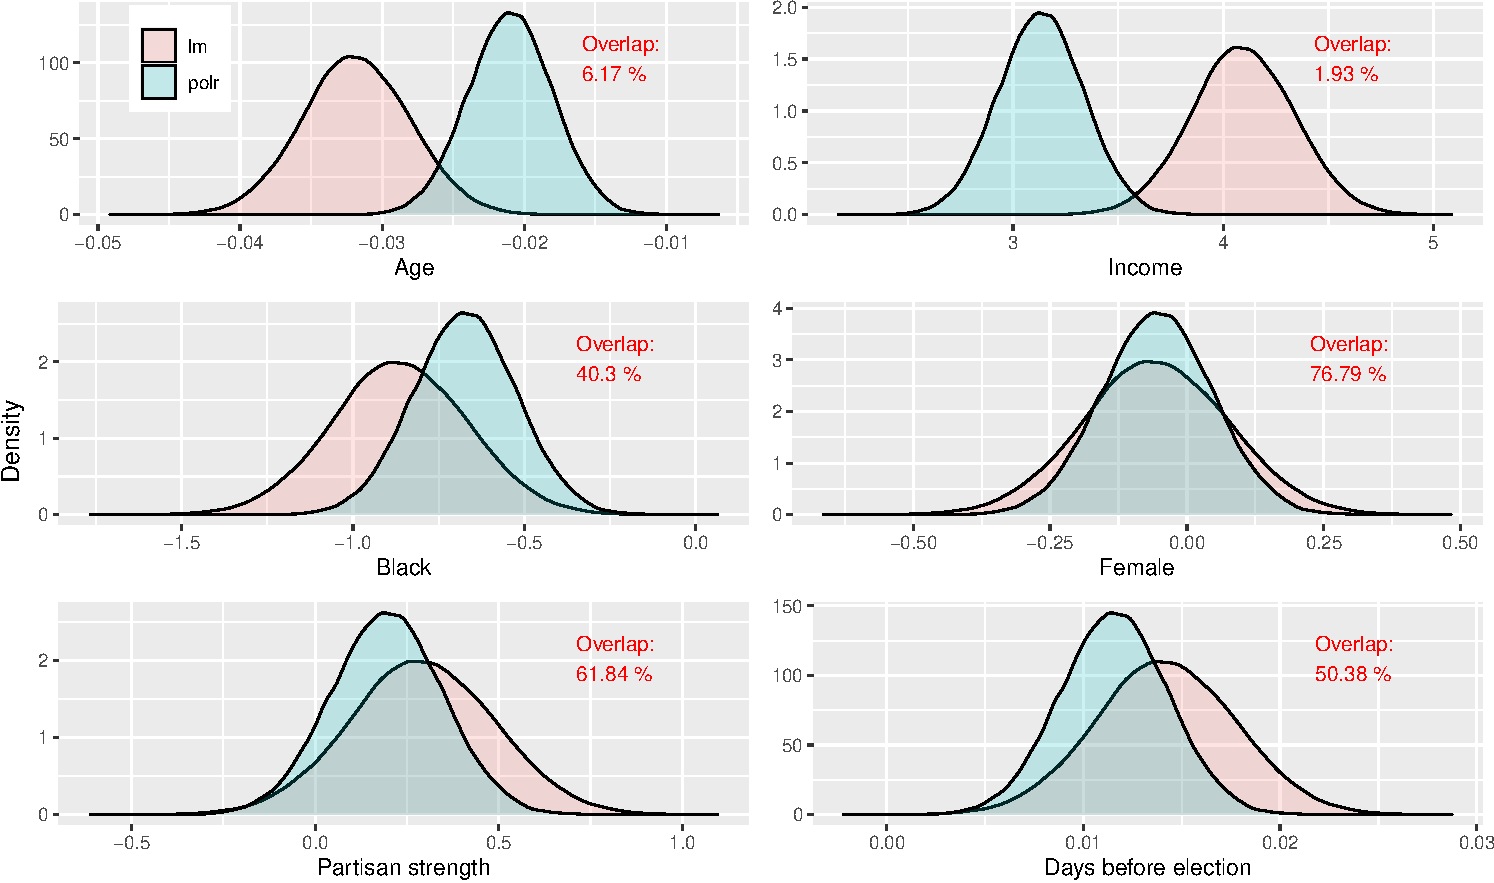
\includegraphics{dissertation_files/figure-latex/Density-Plots-Bartels-1992-1.pdf}
\caption{\label{fig:Density-Plots-Bartels-1992}Distributions of lm and polr coefficients\label{DensBart92}}
\end{figure}
We observe a small posterior percentage of overlay for the distributions of \texttt{Age} and \texttt{Income} (\textless{} 10 percent) and a large posterior percentage of overlay for the distributions of \texttt{Black}, \texttt{Female}, \texttt{Partisan\ strength}, and \texttt{Days\ before\ election} (\textgreater{} 40 percent). Since a large percentage indicates little difference in significance between the two sets of coefficients, these results appear to provide further proof against the importance of re-estimating ordinal variable categories with ordered probit approaches.

Based on evidence from these brief investigative analyses, it thus seems that uneven distances between ordinal variable categories might not actually be of crucial importance when it comes to missing data imputation. These are mere preliminary conclusions, however, and more research is needed to further corroborate this tentative impression.

\hypertarget{ordmiss-conclusion}{%
\section{Conclusion}\label{ordmiss-conclusion}}

I set out to improve multiple imputation results with ordinal variables by accounting for the unevenly spaced ordering contained in ordinal variables. I did so by adapting the multiple hot deck imputation function \texttt{hot.deck} to treat ordinal variables with an ordered probit model in order to estimate numeric thresholds from an assumed underlying latent continuous variable. The results clearly show diverging outcomes from the different algorithms, with each algorithm behaving differently under changing circumstances. While \texttt{hd.ord} did not yield the desired improvements, my analysis provides in-depth insights into and corroborates the robustness of multiple imputation implementations like \texttt{amelia} and \texttt{mice} for a variety of variable types in survey settings.

\texttt{hd.ord} performs on par with some binary variables but overall worse than \texttt{amelia} and \texttt{mice} for data MAR with 5 and with 12 variables with missing values. The difference between the methods is somewhat less pronounced for 12 variables, which could possibly be explained by the thinner spread of missing values across a higher number of variables. The results for the MNAR analyses paint a more mixed but overall unchanged picture. \texttt{hd.ord} performs somewhat better for binary variables but remains the least accurate method for interval and ordinal variables. Increasing the number of ordinal variables included in the \texttt{polr} treatment did not have a positive effect on the performance of \texttt{hd.ord}. In fact, \texttt{hd.ord} consistently performed slightly worse for all variables for both datasets for all mechanisms of missingness. Unlike \texttt{amelia} and \texttt{mice}, \texttt{hd.ord}'s performance also drastically worsens when the percentage of missingness in the data increases to 50 percent and above.

On the positive side, \texttt{hd.ord} performs multiple imputation much more quickly: \texttt{amelia} and \texttt{mice} are at least 3.4 and 19.2 times slower than \texttt{hd.ord} for 20 percent of missing data, respectively. This speed gain is of dubious value, however. While it is necessary to iterate multiple imputation runs many times over for simulation purposes like this one, users likely will not do so, which greatly diminishes the computing time saved. Even if users do opt to run multiple imputation for 1,000 times, the differences in terms of absolute time with \texttt{amelia} are not so great as to be impractical. \texttt{amelia} on average took a little over nine minutes to compute 1,000 iterations of multiple imputation, regardless of the dataset in question. In absolute terms, this is not a lot of time for the general user to invest in data preparation. With an average of around 110 minutes, the same cannot be said for \texttt{mice}. Nonetheless, \texttt{hd.ord}'s speed gain over \texttt{amelia} cannot be considered enough reason to choose \texttt{hd.ord} over \texttt{amelia}, unless the data consists of exclusively binary variables where the difference between \texttt{hd.ord} and \texttt{amelia} are small.

Given all the above, the result of this quality comparison of major missing data solutions is a clear endorsement of \texttt{amelia}. It performs well for all types of variables in all stages of missingness and does so in a reasonably short amount of time. The combination of EM with bootstrapping clearly represents a great improvement in terms of speed over IP used in \texttt{mice}. While it offers a wealth of sophisticated options for specialized users,\texttt{amelia}'s default out-of-the-box settings are simple and intuitive for general users. On top of that, it is notable that \texttt{amelia} produces better results than \texttt{na.omit} when data is MNAR, i.e.~it performs well in a setting it was not designed for. \texttt{amelia} thus represents the best \texttt{R} solution to problems of missing data for general users.

\hypertarget{framing}{%
\chapter{MORAL ARGUMENTS AS A SOURCE OF FRAME STRENGTH}\label{framing}}

Moral conviction literature tells us that people with moralized attitudes hold those attitudes strongly. This indicates that these people's attitudes can't be easily be moved, no matter what frame they are presented with. As a result, we can only move the attitudes of people who don't hold highly moralized attitudes, since there is room for movement here.

(ONE) Give descriptions of what `moral' and `self-interest' is.

Ad hoc examples: ``Moral concerns what people should or should not do'', ``Self-interest concerns actions and attitudes that only suit yourself''.
`Moral' description comes from Ryan, who extended Skitka's moral conviction measure. I extend this further by adding a `self-interest' description, which I still need to find.

(TWO) Ask about respondents' moral conviction towards an issue.

Moral conviction measure from Skitka: ``To what extent is your position on {[}issue{]} a reflection of your core moral beliefs and convictions'' and ``\ldots{} connected to your fundamental beliefs about right and wrong?''.
I ask how `moral' they consider their position on the issue, but without actually asking them what their position is. This is to avoid anchoring.

(THREE) Measure moral conviction towards the issue (1-5 Likert; ``Not at all'', ``Slightly'', ``Moderately'', ``Much'', ``Very much'').

(FOUR) Randomly assign one of the five frames: Opposing moral frame, opposing self-interest frame, control frame, supporting moral frame, supporting self-interest frame.

(FIVE) Measure support/opposition for/to the issue (1-5 Likert; ``Strongly oppose'' \ldots{} ``Strongly approve'').

Expectations:

For the respondents with highly moralized attitudes on the issue, their support/opposition for/to the issue should be statistically the same across all frames, since their attitudes are set and can't easily be moved. For the respondents without highly moralized attitudes on the issue, the frames should move responses towards support or opposition, depending on the direction of the frame. For these people, we can see whether the moral or the self-interest frames cause bigger shifts.

To be gained from this experiment:

-- We can test which issues are considered more moral than others

-- We can test whether people with highly moralized attitudes really stick to their pre-formed attitudes, no matter what they're exposed to

-- We can test whether people with low moralized attitudes are more influenced by moral or self-interest frames

\hypertarget{framing-intro}{%
\section{Introduction}\label{framing-intro}}

Barack Obama presented the first outline of the Affordable Care Act in the summer of 2009. The content of the reform was put online for everyone to see, but since the administration was still working on details, it refrained from actively communicating it. Published press releases simply stated that the ACA would expand coverage and lower health care costs for everyone. This hesitancy turned out to be a big mistake. At the end of July, support for the ACA hovered around 43 percent. Then Sarah Palin, John McCain's choice for running mate in 2008, posted the following statement on Facebook on August 7\textsuperscript{th}: ``The America I know and love is not one in which my parents or my baby with Down Syndrome will have to stand in front of Obama's `death panel' so his bureaucrats can decide, based on a subjective judgment of their `level of productivity in society'\,'' (Palin, 2009). Palin implied that federal government workers would be able to refuse treatment to any patients and thus `decide their fate'. Over the next two weeks, support for the ACA dropped to 35 percent while opposition rose to 52 percent. Republican lawmakers jumped at the opportunity and repeated the claim of `death panels' whenever possible. The reform never recovered from this drop. In December 2009, four months after the statement, support and opposition were virtually identical to August. While the public was still uncertain about the exact contents of the law, Palin had asserted that it would include a Big Brother type panel that decided whether people would live or die. This drowned out any efforts by the Obama administration to show the law as a cost-reducing reform. Palin's frame of the ACA, in other words, drastically influenced public opinion of the reform.

Framing is the practice of presenting an issue to affect the way people see it (Aaroe, 2011; Druckman, 2001a; Gross, 2008). We learn about healthcare reform through articles, reports, speeches, commercials and social media. This mediated communication possesses tremendous potential influence on our perception of political issues (Iyengar, 1996; Kam \& Simas, 2010; Tversky \& Kahneman, 1981). Framing research has established that a variety of frames substantively influence how people view and think about issues, such as the ACA (Andsager, 2000; Callaghan \& Schnell, 2005; Entman, 1993, 2004; Gamson \& Modigliani, 1989; Lahav \& Courtemanche, 2012; Pan \& Kosicki, 1993; Price, Tewksbury, \& Powers, 1997; Slothuus \& Vreese, 2010; Sniderman \& Theriault, 2004; Vreese, 2004). But we do not know why these frames elicit these effects. A major challenge for framing research thus "concerns the identification of factors that make a frame strong'' (Chong \& Druckman, 2007, p. 116).

-- that moral stuff is said to be very powerful
-- that self-interest is said to be very powerful
-- that I'm combining everything.

Both methods developed in chapters II and III are applied in the survey experiment and their performance is analyzed.

\hypertarget{framing-theory}{%
\section{Theory}\label{framing-theory}}

\hypertarget{framing-theory-framing}{%
\subsection{Framing}\label{framing-theory-framing}}

-- Outline differences between equivalency and emphasis frames (I'm looking at emphasis)
-- Outline differences between emphasis frames and new information (Leeper,Slothuus)
-- Clearly express that we do know why frames work (Zaller: Frames move persuasive information to the top of one's mind) but that we don't know why some frames are successful at moving persuasive information to the top of one's mind and others aren't. This was not initially clear to Liz

Despite the mass of experimental framing research, we still have little insight into what makes a frame strong. The larger persuasion literature ``is not as illuminating as one might suppose\ldots{} It is not yet known what it is about the `strong arguments'\ldots{} that makes them persuasive'' (O'Keefe, 2002). One research direction is that frames are stronger overall when they cohere with an individual's personal value system. Feinberg \& Willer (2012) frame environmental issues as a matter of `purity', a theme that supposedly correlates with conservative ideology, and find this approach leads to increased conservative support of environmental policies. (Arceneaux, 2012, p. 280) on the other hand finds that ``individuals are more likely to be persuaded by political arguments that evoke cognitive biases''. Particularly, he asserts that messages which highlight out-group threats resonate to a greater extent than other, more coherent, arguments. In a study investigating the use of scientific data, Druckman \& Bolsen (2011) report that adding factual information to messages about carbon nanotubes does nothing to enhance their strength. Providing more scientific evidence seems to have the opposite effect, making the messages weaker. Overall, ``it seems as if frame strength increases with frames that highlight specific emotions, invoke threat against one's own group interests, contain some incivility, include multiple, frequently appearing, arguments, and/or have been used in the past'' (Druckman, Klar, Robison, \& Gubitz, 2018, p. 22). I attempt to provide an avenue of clarification by testing whether moral arguments are part of what makes frames strong.

\hypertarget{framing-theory-morality-self_interest}{%
\subsection{Morality and Self-Interest}\label{framing-theory-morality-self_interest}}

(Stoker, 1992):
Central claim of economic theory: homo economicus, i.e.~the rational man who pursues his selfish interests (Coleman, 1986). There is weak and little evidence for that (Citrin \& Green, 1990; Mansbridge, 1980; Sears \& Funk, 1990). In a follow-up approach, rational choice theorists claim people simply want to maximize their utility, defining self-interest to include material and immaterial, selfish and altruistic interests (Arrow, 1967; Downs, 1957; Olson, 1965; Opp, 1989). A competing direction defines self-interest narrowly in a contrast between selfish and non-selfish preferences, highlighting the significance of non-selfish motives such as love (Mansbridge, 1990), sympathy (Sen, 1977), and justice (Tyler, 1990). The first apprach casts a wide net and says that people seek whatever they find to be in their interest. People pursue their interests but those interests may include non-selfish ones. The second equals self-interest with self-regarding and juxtaposes self-regarding interests with non-egoist ones. Non-egoist interests are here conceptually different from self-regarding ones. Stoker argues that people don't just want to satisfy their preferences (self-regarding or not self-regarding), but neither do they set aside their self-regarding preferences in favor of some non-self-regarding ones. Instead, they deal with the `central problem of ethics': ``how the lives, interests, and welfare of others make claims on us, and how these claims, of various forms, are to be reconciled with the aim of living our own lives'' (Nagel, 1970, p. 142). Stoker paints citizens as ethical actors.

ME: I ask people to assess issues on relevant moral grounds and in self-interest terms of the consequences for their lives. Then we can see whether people vary in their view of whether a policy advances their interests and whether people differ in the weight they give to different moral criteria when forming policy opinions.

Unenlightened self-interest (Bartels, 2005): A majority of Americans supported the 2001 and 2003 Bush administration tax cuts, even though they were designed to disproportionately benefit the rich. Economic self-interest can't explain this, since the majority of Americans suffered economically from the cuts. As Bartels shows, neither can people's attitudes towards the tax burden born by the rich. Instead, attitude towards the tax cuts was shaped by respodnents' perceived self-interest: The tax burden they had to endure. In grossly exaggerated terms: They felt their tax burden was too high, so they supported the tax cuts, even though, in material terms, the cuts hurt them. Bartels call this ``unenlightened self-interest'' (p.~23). Bartels further shows that highly informed respondents had a very different attitude: They overwhelmingly opposed the cuts. He suggests that it may be unreasonable to expect Americans to make informed decisions on highly complex issues such as tax reform, which is why they might revert to subjective perception (unenlightened self-interest) rather than objective calculation (material self-interest).

Moralization literature conceptually defines moral arguments as (1) near-universal standards of truth, (2) almost objective facts about the world, and (3) independent of institutional authority (Skitka, 2010).
Moral arguments are said to engage a distinctive mode of processing that invokes a whole range of emotions and to be distinct from other forms of arguments (Ryan, 2014b).
Scholars find that moral arguments are ubiquitous in political issues because they are essential to how people perceive and make sense of the world around them (Frank, 2005; Mooney, 2001; Tatalovich, Smith, \& Bobic, 1994).
Ryan (2014b) finds evidence that some people perceive distinctly economic issues such as labor relations laws or social security reform in moral ways.
Other studies similarly assert that the strength of attitudes meaningfully differs when they are held with moral conviction (Baron \& Spranca, 1997; Bennis, Medin, \& Bartels, 2010; Ditto, Pizarro, \& Tannenbaum, 2009; Tetlock, 2003).
It is also asserted that moral conviction represents an important force that guides citizen behavior and development of public opinion (Converse, 1964; Skitka, Bauman, \& Sargis, 2005; Skitka \& Wisneski, 2011; Smith, 2002; Tatalovich \& Daynes, 2011; Zaller, 1992).
It is widely argued that people rely to a disproportionate extent on moral arguments to form their opinions and apply this moralization to political issues (Ryan, 2014a, 2014b; Smith, 2002).
Moral arguments can achieve a much higher emotional connection with people because they invoke people's values and feelings (Haidt, 2003; Skitka et al., 2005; Skitka \& Wisneski, 2011; Tatalovich \& Daynes, 2011).
These conceptual definitions are all encompassed in Moral Foundations Theory (MFT), developed by Haidt (2012) and presented in Table \ref{framing-foundations} below.
\begin{table}[ht]
\caption{Foundations of Moral Arguments}
\centering
\resizebox{\textwidth}{!}{
\begin{tabular}{>{\itshape}l ll >{\itshape}l l}
\bottomrule 
\midrule
\multicolumn{2}{c}{\textbf{Positive}} & & \multicolumn{2}{c}{\textbf{Negative}}\\
\cmidrule{1-2}
\cmidrule{4-5}
Care & Cherishing, protecting others & & Harm & Hurting others\\
Fairness & Rendering justice by shared rules & & Cheating & Flouting justice, shared rules\\
Loyalty & Standing with your group & & Betrayal & Opposing your group\\
Respect & Submitting to tradition, authority & & Subversion & Resisting tradition, authority\\
Sanctity & Repulsion at disgust & & Degradation & Enjoyment of disgust \\
\bottomrule
\multicolumn{5}{l}{\footnotesize{Based on Haidt (2012). Positive and negative foundations are conceptual opposites.}} \\
\end{tabular}}
\label{framing-foundations}
\end{table}
These aspects of moralization theory have not been applied to frame strength in experimental research. An abundance of framing research has shown that frames elicit significant changes in issue positioning (Chong \& Druckman, 2010, 2013; Druckman, 2001b; Druckman, Fein, \& Leeper, 2012; Druckman et al., 2013; Nelson, Clawson, \& Oxley, 1997; Slothuus, 2008). Brewer \& Gross (2005), for instance, find significant effects for the frames `School vouchers create an unfair advantage' and `School vouchers provide help for those who need it'. Druckman et al. (2012) provide similar evidence for `The Affordable Care Act gives more people equal access to health insurance' and `The ACA increases government costs', while Druckman et al. (2013) do so for `Oil drilling provides economic benefits' and `Oil drilling endangers marine life'. While we know these frames elicit changes, we do not know why they do so. We do not know why these frames `work'. I propose a way to understand why some of these frames work, which is based on moralization theory: The presence of moral arguments.

Applying Moral Foundation Theory, both frames in Brewer \& Gross (2005) could be categorized as containing moral arguments, even though the authors do not explicitly do so. `School vouchers create an unfair advantage' can be argued to contain the negative moral foundation of \textit{Cheating}, while `School vouchers provide help for those who need it' contains the positive moral foundations of \textit{Care} and \textit{Fairness}. `The ACA gives more people equal access to health insurance' (Druckman et al., 2012) also could be said to contain the positive moral foundations of \textit{Care} and \textit{Fairness}, while `Oil drilling endangers marine life' (Druckman et al., 2013) contains the negative moral foundation of \textit{Harm}.

It is important to note that `The ACA increases government costs' (Druckman et al., 2012) and `Oil drilling provides economic benefits' (Druckman et al., 2013) do not directly appeal to morality, yet research has shown them to be strong. Of course, some people might see increasing costs immediately as bad and thus morally detrimental for the future of the country, but these frames do not make such an appeal directly, on the surface. This distinguishes them from moral frames.

This might lead one to assert that moral arguments do not form a part of frame strength -- after all, if a frame does not contain a direct moral argument but is proven to be strong nonetheless, surely then frame strength does not depend on the presence of moral arguments. This hypothetical argument is flawed, however. For one, the search for the source of frame strength is not the search for a universal `holy grail' argument whose presence is a precondition for frame strength. There probably are many aspects that can make a frame strong, with moral arguments potentially being one of them, not the only one. Second, the studies with these two amoral and two moral arguments do not distinguish between the directions in which the moral and amoral frames act.

In the case of Druckman et al. (2012), `The Affordable Care Act gives more people equal access to health insurance' contains a positive, i.e.~support-inducing, moral argument, while `The ACA increases government costs' contains a negative, i.e.~opposition-inducing, amoral argument. They act in opposite directions. A comparison of these frames alone does not yield sufficient results as we would not be able to identify the exact cause of the framing effect. Is `The Affordable Care Act gives more people equal access to health insurance' strong because it supports the issue or because it contains a moral argument? Similarly, is `The ACA increases government costs' strong because it opposes the issue or because it contains a amoral argument? This set-up cannot answer these questions.

To establish whether moral arguments are part of what makes a frame strong, we need a design that assesses the strength of frames with moral and amoral arguments whilst accounting for both signs, opposing and supporting, in both sets of frames. I provide such a design.

Overall, experimental framing research has shown that many frames have significant framing effects. It is still unclear, however, what makes these, or indeed any, frame strong (Druckman et al., 2018). Moralization theory claims that moral arguments possess enormous power shape human behavior and influence public opinion (Haidt, 2003). I combine these two sets of literature and analyze whether moral arguments form a part of what makes frames strong. I use a variety of data sources to investigate the following hypothesis:

\hypertarget{framing-theory-hypothesis}{%
\subsection{Hypothesis}\label{framing-theory-hypothesis}}

\vspace{0.3cm}
\begin{adjustwidth*}{+1cm}{+1cm}
\textbf{H.} Moral arguments form a part of what makes political frames strong.
\end{adjustwidth*}
\hypertarget{framing-data}{%
\section{Data}\label{framing-data}}

\hypertarget{framing-data-pre_test}{%
\subsection{Pre-Tests}\label{framing-data-pre_test}}

Survey questions are best designed if researchers have a firm grasp of the underlying realities that participants have to report (Carpini \& Keeter, 1993; Conover, Crewe, \& Searing, 1991; Stanley, 2016). Following this line of argument, pre-testing frames with participants who are not part of the main survey experiment is crucial in frame analysis. These participants are exposed to the designed frames and asked whether they reflect the core ideas behind `moral' and `self-interest'. This pre-test structure builds on work by Slothuus \& Vreese (2010) and Chong \& Druckman (2007), following the mass communication and persuasion literature (O'Keefe, 2002). The pre-test is carried out on Amazon's online platform MTurk. MTurk is a service where researchers can host tasks to be completed by anonymous participants. Participants receive financial compensation for their work and Amazon collects a commission. MTurk samples have been shown to be internally valid in survey experiments (Berinsky, Huber, \& Lenz, 2012). The use of MTurk in political science experiments has increased dramatically over the past decade and is now common practice (Hauser \& Schwarz, 2016). This pre-test represents a thorough, robust safety net to ensure that the designed frames connect with participants, which in turn ensures meaningful survey results.

\hypertarget{framing-data-survey}{%
\subsection{Survey Experiment}\label{framing-data-survey}}

The survey experiment builds on the insights from the pre-test. It is fielded online for a random sample of U.S. adults with Lucid. Lucid has been shown to be equally reliable and performs well on a national scale in survey experiments (Coppock \& McClellan, 2019).
The experiment features frames with `moral' and `self-interest' arguments, reflecting the respective descriptions.
The survey also collects demographic information on standard political science variables.
The selected issues are chosen from previous research. The form a combination of big-hitter issues (gay marriage, abortion, climate change) and smaller issues (TBD) where you can move the needle.
Respondents are blocked on ordinal variables with the method from chapter I. As part of the analysis, the ordinal variable imputation method from chapter II is applied to inserted missing data. We can assess the performance of ordinal variable imputation method because we know the true values of the completely observed data.

\hypertarget{framing-results}{%
\section{Results}\label{framing-results}}

\hypertarget{framing-results-imputation}{%
\subsection{Imputation}\label{framing-results-imputation}}

\hypertarget{framing-conclusion}{%
\section{Conclusion}\label{framing-conclusion}}

\hypertarget{conclusion}{%
\chapter{CONCLUSION}\label{conclusion}}

Education is the most important predictor of political behavior in political science. It is crucial that we measure and use this variable correctly to obtain results that reflect the true data structure. As an ordinal variable, education contains special characteristics: Its categories are ordered, but unevenly spaced. We need modern statistical methods to fully utilize all this information contained in this variable. So far, this aspect has been largely ignored in the literature. If we want to know what people think and how they act, we need to make sure our measurements are as good as they can possibly be. My dissertation outlines two new methods that contribute to this undertaking. They significantly improve how we handle ordinal variables in surveys and survey experiments in political science and thus increase precision when we analyze public opinion.

Whether my methods are suitable in a specific survey or survey experiment depends on the situation, as no method works for all circumstances. For a survey experiment with a very large sample and few treatment groups, there is no need for my ordered probit method and blocking. Simple randomization does the job here. Similarly, if survey results do not contain important ordinal predictor variables, my method to impute missing data from ordinal variables is not applicable. Overall, my dissertation adds two important new tools to the empirical political scientist's toolbox to choose from.

\appendix

\hypertarget{app-ordblock}{%
\chapter{ORDINAL BLOCKING}\label{app-ordblock}}

In order to conduct this experiment, I created an online survey environment based on \texttt{R} with \texttt{shiny} (Boas \& Hidalgo, 2013), as there currently is no available tool to block sequentially online. Popular online survey platforms, such as Qualtrics, do not have offer this functionality, and none of the attempts to combine \texttt{R} code work with Qualtrics concern the `injection' of \texttt{R} code into the Qualtrics randomization engine, which blocking would require (Barari et al., 2017; Ginn, 2018; Hainmueller, Hopkins, \& Yamamoto, 2014; Testa, 2017). The following is a basic outline of the mechanisms behind this survey environment.

The survey questions, i.e.~questions that collect demographic information and questions that apply treatment, need to be designed as \texttt{.txt} files and incorporated into a local \texttt{shiny} environment. This local environment is then hosted in the cloud and publicly accessible. The hosted website sequentially blocks each incoming participant based on her covariate information and covariate information from all previous participants through constant interaction with the \texttt{R} code. The workflow for any incoming participant is illustrated in Figure \ref{online-workflow} below.

\vspace{0.8cm}
\begin{figure}[ht]
\centering
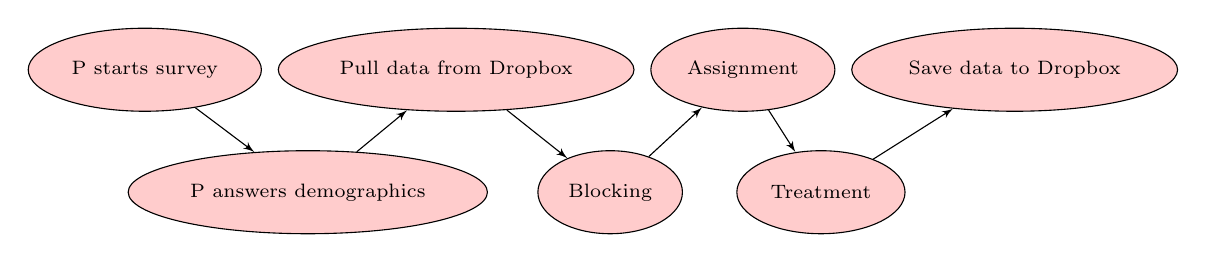
\begin{tikzpicture}
    \node [cloud]  (survey) {\scriptsize{P starts survey}};
    \node [cloud, below right=0.8cm and -0.6cm of survey] (dems) {\scriptsize{P answers demographics}};
    \node [cloud, right= 0.2cm of survey] (pulls) {\scriptsize{Pull data from Dropbox}};
    \node [cloud, below right=0.8cm and -0.3cm of pulls] (blocking) {\scriptsize{Blocking}};
    \node [cloud, right= 0.2cm of pulls] (assignment) {\scriptsize{Assignment}};
    \node [cloud, below right=0.8cm and -0.6cm of assignment] (treatment) {\scriptsize{Treatment}};
    \node [cloud, right= 0.2cm of assignment] (results) {\scriptsize{Save data to Dropbox}};
    \path [line] (survey) -- (dems);
    \path [line] (dems) -- (pulls);
    \path [line] (pulls) -- (blocking);
    \path [line] (blocking) -- (assignment);
    \path [line] (assignment) -- (treatment);
    \path [line] (treatment) -- (results);
\end{tikzpicture}
\caption{Online survey experiment workflow} \label{online-workflow}
\end{figure}
A participant clicks on the survey link and answers the demographic question. After she selects her level of education, \texttt{R} code in the background pulls previous participants' covariate information from a Dropbox server. Based on this information and her chosen education level, the \texttt{R} code sequentially blocks and assigns her to a treatment group. The participant then sees and answers the respective treatment question(s). Her responses are then saved on the same Dropbox server. This process is repeated for all incoming participants. If the participant is the first person to take the survey, i.e.~if there is no covariate information from previous participants yet, the code randomly assigns her to one of the treatment groups. All subsequent participants are then blocked and assigned as just described. To recruit participants, the cloud-based website can easily be linked to online market platforms, such as MTurk or Lucid.

\hypertarget{app-ordmiss}{%
\chapter{ORDINAL MISSING}\label{app-ordmiss}}

\hypertarget{app-ordmiss-allObs}{%
\section{All Observations}\label{app-ordmiss-allObs}}

ANES all obs. 1000 iterations, CCES all obs. 10 iterations (maxed out RAM)
5 variables: Dem, Male, Interest, Inc, Age
MAR (Table \ref{mar.5var.all}) and MNAR (\ref{mnar.5var.all})
\begin{table}[!htbp] \centering 
  \caption{Accuracy of Multiple Imputation Methods. MAR, 5 Variables with NA, all observations} 
  \label{mar.5var.all} 
\begin{threeparttable}
\begin{tabular}{@{\extracolsep{5pt}} D{.}{.}{-3} D{.}{.}{-3} D{.}{.}{-3} D{.}{.}{-3} } 
\\[-1.8ex]\hline 
\hline \\[-1.8ex] 
\multicolumn{1}{c}{Method} & \multicolumn{1}{c}{Variable} & \multicolumn{1}{c}{ANES} & \multicolumn{1}{c}{CCES} \\ 
\hline \\[-1.8ex] 
\multicolumn{1}{c}{true} & \multicolumn{1}{c}{Dem} & \multicolumn{1}{c}{.3370} & \multicolumn{1}{c}{.4032} \\ 
\multicolumn{1}{c}{hot.deck} & \multicolumn{1}{c}{Dem} & \multicolumn{1}{c}{--.0001} & \multicolumn{1}{c}{+.0006} \\ 
\multicolumn{1}{c}{hd.ord} & \multicolumn{1}{c}{Dem} & \multicolumn{1}{c}{--.0002} & \multicolumn{1}{c}{+.0006} \\ 
\multicolumn{1}{c}{amelia} & \multicolumn{1}{c}{Dem} & \multicolumn{1}{c}{+.0000} & \multicolumn{1}{c}{+.0003} \\ 
\multicolumn{1}{c}{mice} & \multicolumn{1}{c}{Dem} & \multicolumn{1}{c}{+.0000} & \multicolumn{1}{c}{+.0003} \\ 
\multicolumn{1}{c}{na.omit} & \multicolumn{1}{c}{Dem} & \multicolumn{1}{c}{--.0302} & \multicolumn{1}{c}{--.0250} \\ 
\multicolumn{1}{c}{true} & \multicolumn{1}{c}{Male} & \multicolumn{1}{c}{.4868} & \multicolumn{1}{c}{.4521} \\ 
\multicolumn{1}{c}{hot.deck} & \multicolumn{1}{c}{Male} & \multicolumn{1}{c}{--.0004} & \multicolumn{1}{c}{--.0001} \\ 
\multicolumn{1}{c}{hd.ord} & \multicolumn{1}{c}{Male} & \multicolumn{1}{c}{--.0008} & \multicolumn{1}{c}{--.0002} \\ 
\multicolumn{1}{c}{amelia} & \multicolumn{1}{c}{Male} & \multicolumn{1}{c}{+.0001} & \multicolumn{1}{c}{+.0001} \\ 
\multicolumn{1}{c}{mice} & \multicolumn{1}{c}{Male} & \multicolumn{1}{c}{+.0001} & \multicolumn{1}{c}{+.0001} \\ 
\multicolumn{1}{c}{na.omit} & \multicolumn{1}{c}{Male} & \multicolumn{1}{c}{--.0365} & \multicolumn{1}{c}{--.0436} \\ 
\multicolumn{1}{c}{true} & \multicolumn{1}{c}{Interest} & \multicolumn{1}{c}{2.8806} & \multicolumn{1}{c}{3.3301} \\ 
\multicolumn{1}{c}{hot.deck} & \multicolumn{1}{c}{Interest} & \multicolumn{1}{c}{--.0087} & \multicolumn{1}{c}{--.0033} \\ 
\multicolumn{1}{c}{hd.ord} & \multicolumn{1}{c}{Interest} & \multicolumn{1}{c}{--.0135} & \multicolumn{1}{c}{--.0046} \\ 
\multicolumn{1}{c}{amelia} & \multicolumn{1}{c}{Interest} & \multicolumn{1}{c}{+.0001} & \multicolumn{1}{c}{+.0001} \\ 
\multicolumn{1}{c}{mice} & \multicolumn{1}{c}{Interest} & \multicolumn{1}{c}{+.0000} & \multicolumn{1}{c}{+.0000} \\ 
\multicolumn{1}{c}{na.omit} & \multicolumn{1}{c}{Interest} & \multicolumn{1}{c}{--.0741} & \multicolumn{1}{c}{--.0763} \\ 
\multicolumn{1}{c}{true} & \multicolumn{1}{c}{Inc} & \multicolumn{1}{c}{16.6894} & \multicolumn{1}{c}{6.5830} \\ 
\multicolumn{1}{c}{hot.deck} & \multicolumn{1}{c}{Inc} & \multicolumn{1}{c}{--.0606} & \multicolumn{1}{c}{--.0009} \\ 
\multicolumn{1}{c}{hd.ord} & \multicolumn{1}{c}{Inc} & \multicolumn{1}{c}{--.1030} & \multicolumn{1}{c}{--.0073} \\ 
\multicolumn{1}{c}{amelia} & \multicolumn{1}{c}{Inc} & \multicolumn{1}{c}{+.0009} & \multicolumn{1}{c}{--.0021} \\ 
\multicolumn{1}{c}{mice} & \multicolumn{1}{c}{Inc} & \multicolumn{1}{c}{--.0007} & \multicolumn{1}{c}{--.0022} \\ 
\multicolumn{1}{c}{na.omit} & \multicolumn{1}{c}{Inc} & \multicolumn{1}{c}{--.5574} & \multicolumn{1}{c}{--.2592} \\ 
\multicolumn{1}{c}{true} & \multicolumn{1}{c}{Age} & \multicolumn{1}{c}{50.3745} & \multicolumn{1}{c}{52.8639} \\ 
\multicolumn{1}{c}{hot.deck} & \multicolumn{1}{c}{Age} & \multicolumn{1}{c}{--.2355} & \multicolumn{1}{c}{--.0221} \\ 
\multicolumn{1}{c}{hd.ord} & \multicolumn{1}{c}{Age} & \multicolumn{1}{c}{--.3698} & \multicolumn{1}{c}{--.0790} \\ 
\multicolumn{1}{c}{amelia} & \multicolumn{1}{c}{Age} & \multicolumn{1}{c}{+.0056} & \multicolumn{1}{c}{--.0006} \\ 
\multicolumn{1}{c}{mice} & \multicolumn{1}{c}{Age} & \multicolumn{1}{c}{+.0053} & \multicolumn{1}{c}{--.0132} \\ 
\multicolumn{1}{c}{na.omit} & \multicolumn{1}{c}{Age} & \multicolumn{1}{c}{--1.2785} & \multicolumn{1}{c}{--1.2190} \\ 
\hline \\[-1.8ex] 
\multicolumn{2}{c}{Observations} & \multicolumn{1}{c}{2395} & \multicolumn{1}{c}{42205} \\ 
\multicolumn{2}{c}{Iterations} & \multicolumn{1}{c}{1000} & \multicolumn{1}{c}{10} \\ 
\hline \\[-1.8ex] 
\end{tabular} 
\begin{tablenotes}[para,flushleft]
\footnotesize{\textit{Note:} Due to the very high number of observations, the CCES data can only be run for a low number of iterations. Anything above that maxes out the 120 GB of RAM available to me. The framing data are not included since their total number of observations (1,003) is virtually identical to the sample of 1,000.}
\end{tablenotes}
\end{threeparttable}
\end{table}
\begin{table}[!htbp] \centering 
  \caption{Accuracy of Multiple Imputation Methods. MNAR, 5 Variables with NA, all observations} 
  \label{mnar.5var.all} 
\begin{threeparttable}
\begin{tabular}{@{\extracolsep{5pt}} D{.}{.}{-3} D{.}{.}{-3} D{.}{.}{-3} D{.}{.}{-3} } 
\\[-1.8ex]\hline 
\hline \\[-1.8ex] 
\multicolumn{1}{c}{Method} & \multicolumn{1}{c}{Variable} & \multicolumn{1}{c}{ANES} & \multicolumn{1}{c}{CCES} \\ 
\hline \\[-1.8ex] 
\multicolumn{1}{c}{true} & \multicolumn{1}{c}{Dem} & \multicolumn{1}{c}{.3370} & \multicolumn{1}{c}{.4032} \\ 
\multicolumn{1}{c}{hot.deck} & \multicolumn{1}{c}{Dem} & \multicolumn{1}{c}{--.0109} & \multicolumn{1}{c}{--.0105} \\ 
\multicolumn{1}{c}{hd.ord} & \multicolumn{1}{c}{Dem} & \multicolumn{1}{c}{--.0113} & \multicolumn{1}{c}{--.0105} \\ 
\multicolumn{1}{c}{amelia} & \multicolumn{1}{c}{Dem} & \multicolumn{1}{c}{--.0110} & \multicolumn{1}{c}{--.0109} \\ 
\multicolumn{1}{c}{mice} & \multicolumn{1}{c}{Dem} & \multicolumn{1}{c}{--.0103} & \multicolumn{1}{c}{--.0106} \\ 
\multicolumn{1}{c}{na.omit} & \multicolumn{1}{c}{Dem} & \multicolumn{1}{c}{--.0185} & \multicolumn{1}{c}{--.0145} \\ 
\multicolumn{1}{c}{true} & \multicolumn{1}{c}{Male} & \multicolumn{1}{c}{.4868} & \multicolumn{1}{c}{.4521} \\ 
\multicolumn{1}{c}{hot.deck} & \multicolumn{1}{c}{Male} & \multicolumn{1}{c}{--.0138} & \multicolumn{1}{c}{--.0129} \\ 
\multicolumn{1}{c}{hd.ord} & \multicolumn{1}{c}{Male} & \multicolumn{1}{c}{--.0136} & \multicolumn{1}{c}{--.0131} \\ 
\multicolumn{1}{c}{amelia} & \multicolumn{1}{c}{Male} & \multicolumn{1}{c}{--.0134} & \multicolumn{1}{c}{--.0132} \\ 
\multicolumn{1}{c}{mice} & \multicolumn{1}{c}{Male} & \multicolumn{1}{c}{--.0134} & \multicolumn{1}{c}{--.0131} \\ 
\multicolumn{1}{c}{na.omit} & \multicolumn{1}{c}{Male} & \multicolumn{1}{c}{--.0196} & \multicolumn{1}{c}{--.0244} \\ 
\multicolumn{1}{c}{true} & \multicolumn{1}{c}{Interest} & \multicolumn{1}{c}{2.8806} & \multicolumn{1}{c}{3.3301} \\ 
\multicolumn{1}{c}{hot.deck} & \multicolumn{1}{c}{Interest} & \multicolumn{1}{c}{--.0257} & \multicolumn{1}{c}{--.0171} \\ 
\multicolumn{1}{c}{hd.ord} & \multicolumn{1}{c}{Interest} & \multicolumn{1}{c}{--.0299} & \multicolumn{1}{c}{--.0179} \\ 
\multicolumn{1}{c}{amelia} & \multicolumn{1}{c}{Interest} & \multicolumn{1}{c}{--.0178} & \multicolumn{1}{c}{--.0147} \\ 
\multicolumn{1}{c}{mice} & \multicolumn{1}{c}{Interest} & \multicolumn{1}{c}{--.0179} & \multicolumn{1}{c}{--.0148} \\ 
\multicolumn{1}{c}{na.omit} & \multicolumn{1}{c}{Interest} & \multicolumn{1}{c}{--.0407} & \multicolumn{1}{c}{--.0418} \\ 
\multicolumn{1}{c}{true} & \multicolumn{1}{c}{Inc} & \multicolumn{1}{c}{16.6894} & \multicolumn{1}{c}{6.5830} \\ 
\multicolumn{1}{c}{hot.deck} & \multicolumn{1}{c}{Inc} & \multicolumn{1}{c}{--.1874} & \multicolumn{1}{c}{--.0691} \\ 
\multicolumn{1}{c}{hd.ord} & \multicolumn{1}{c}{Inc} & \multicolumn{1}{c}{--.2287} & \multicolumn{1}{c}{--.0696} \\ 
\multicolumn{1}{c}{amelia} & \multicolumn{1}{c}{Inc} & \multicolumn{1}{c}{--.1292} & \multicolumn{1}{c}{--.0637} \\ 
\multicolumn{1}{c}{mice} & \multicolumn{1}{c}{Inc} & \multicolumn{1}{c}{--.1297} & \multicolumn{1}{c}{--.0634} \\ 
\multicolumn{1}{c}{na.omit} & \multicolumn{1}{c}{Inc} & \multicolumn{1}{c}{--.2729} & \multicolumn{1}{c}{--.1375} \\ 
\multicolumn{1}{c}{true} & \multicolumn{1}{c}{Age} & \multicolumn{1}{c}{50.3745} & \multicolumn{1}{c}{52.8639} \\ 
\multicolumn{1}{c}{hot.deck} & \multicolumn{1}{c}{Age} & \multicolumn{1}{c}{--.5240} & \multicolumn{1}{c}{--.2331} \\ 
\multicolumn{1}{c}{hd.ord} & \multicolumn{1}{c}{Age} & \multicolumn{1}{c}{--.6609} & \multicolumn{1}{c}{--.2764} \\ 
\multicolumn{1}{c}{amelia} & \multicolumn{1}{c}{Age} & \multicolumn{1}{c}{--.2533} & \multicolumn{1}{c}{--.2342} \\ 
\multicolumn{1}{c}{mice} & \multicolumn{1}{c}{Age} & \multicolumn{1}{c}{--.2474} & \multicolumn{1}{c}{--.2371} \\ 
\multicolumn{1}{c}{na.omit} & \multicolumn{1}{c}{Age} & \multicolumn{1}{c}{--.7188} & \multicolumn{1}{c}{--.6476} \\ 
\hline \\[-1.8ex] 
\multicolumn{2}{c}{Observations} & \multicolumn{1}{c}{2395} & \multicolumn{1}{c}{42205} \\ 
\multicolumn{2}{c}{Iterations} & \multicolumn{1}{c}{1000} & \multicolumn{1}{c}{10} \\ 
\hline \\[-1.8ex] 
\end{tabular} 
\begin{tablenotes}[para,flushleft]
\footnotesize{\textit{Note:} Due to the very high number of observations, the CCES data can only be run for a low number of iterations. Anything above that maxes out the 120 GB of RAM available to me. The framing data are not included since their total number of observations (1,003) is virtually identical to the sample of 1,000.}
\end{tablenotes}
\end{threeparttable}
\end{table}
\clearpage

\hypertarget{app-ordmiss-increaseNA}{%
\section{Increased Missingness}\label{app-ordmiss-increaseNA}}

CCES 10,000 iterations +++
5 variables: Dem, Male, Interest, Inc, Age
MAR
20, 50 percent

\hypertarget{app-ordmiss-speed}{%
\section{Speed}\label{app-ordmiss-speed}}

CCES 10,000 iterations +++
5 variables: Dem, Male, Interest, Inc, Age
MAR
20, 50 percent
\begin{table}[!htbp] \centering 
  \caption{Runtimes of Multiple Imputation Methods (in Minutes) with All Available Observations} 
  \label{run.all.obs} 
\begin{threeparttable}
\begin{tabular}{@{\extracolsep{5pt}} D{.}{.}{-3} D{.}{.}{-3} D{.}{.}{-3} } 
\\[-1.8ex]\hline 
\hline \\[-1.8ex] 
\multicolumn{1}{c}{Method} & \multicolumn{1}{c}{ANES} & \multicolumn{1}{c}{CCES} \\ 
\hline \\[-1.8ex] 
\multicolumn{1}{c}{hd.ord} & \multicolumn{1}{c}{9.406} & \multicolumn{1}{c}{21.829} \\ 
\multicolumn{1}{c}{hot.deck} & \multicolumn{1}{c}{9.374} & \multicolumn{1}{c}{21.429} \\ 
\multicolumn{1}{c}{amelia} & \multicolumn{1}{c}{12.393} & \multicolumn{1}{c}{2.602} \\ 
\multicolumn{1}{c}{mice} & \multicolumn{1}{c}{99.455} & \multicolumn{1}{c}{100.253} \\ 
\hline \\[-1.8ex] 
\multicolumn{1}{c}{Observations} & \multicolumn{1}{c}{2395} & \multicolumn{1}{c}{42205} \\ 
\multicolumn{1}{c}{Iterations} & \multicolumn{1}{c}{1000} & \multicolumn{1}{c}{10} \\ 
\hline \\[-1.8ex] 
\end{tabular} 
\begin{tablenotes}[para,flushleft]
\footnotesize{\textit{Note:} Due to the very high number of observations, the CCES data can only be run for a low number of iterations. Anything above that maxes out the 120 GB of RAM available to me. The framing data are not included since their total number of observations (1,003) is virtually identical to the sample of 1,000.}
\end{tablenotes}
\end{threeparttable}
\end{table}
\begin{table}[!htbp] \centering 
  \caption{Runtimes of Multiple Imputation Methods (in Minutes)} 
  \label{runtimes} 
\begin{tabular}{@{\extracolsep{5pt}} D{.}{.}{-3} D{.}{.}{-3} D{.}{.}{-3} D{.}{.}{-3} D{.}{.}{-3} } 
\\[-1.8ex]\hline 
\hline \\[-1.8ex] 
 & \multicolumn{1}{c}{OldFraming} & \multicolumn{1}{c}{ANES2016} & \multicolumn{1}{c}{ANES2016\_5lev} & \multicolumn{1}{c}{OldFramingQuadrObs} \\ 
\cline{2-2} 
\cline{3-3} 
\cline{4-4}
\cline{5-5}\\[-1.8ex]
\multicolumn{1}{c}{hd.ord} & 34.457 & 32.642 & 32.668 & 31.519 \\ 
\multicolumn{1}{c}{hd.norm} & 34.660 & 32.669 & 32.881 & 31.810 \\ 
\multicolumn{1}{c}{amelia} & 77.956 & 33.051 & 33.691 & 30.035 \\ 
\multicolumn{1}{c}{mice} & 616.023 & 293.722 & 298.919 & 277.021 \\ 
\hline \\[-1.8ex] 
\multicolumn{1}{c}{Observations} & 1,003 & 3,223 & 3,145 & 4,012 \\ 
\multicolumn{1}{c}{Iterations} & 12,500 & 2,396 & 2,500 & 1,500 \\ 
\multicolumn{1}{c}{Levels} & 7 & 16 & 5 & 7 \\ 
\hline \\[-1.8ex] 
\end{tabular} 
\end{table}
As can be seen in Table \ref{runtimes}, \texttt{hd.ord} and \texttt{hot.deck} show virtually identical imputation times for the old framing data (n = 1,003), with \texttt{hd.ord} being 12 seconds faster. \texttt{amelia}, however, is 2.3 times slower than \texttt{hd.ord}. \texttt{mice} is 17.9 times slower than \texttt{hd.ord}. This is a dramatic speed gain. The ANES (n = 3,223) data show only a reduced speed gain. \texttt{mice} is still drastically slower than \texttt{hd.ord} (by a magnitude of 9), but the speed gain is cut in half. The previous speed gain over \texttt{amelia} is no longer observable. \texttt{hd.ord} and \texttt{amelia} now show virtually identical runtimes (with a difference of 25 seconds in favor of \texttt{hd.ord}).

Three factors might explain this sudden and surprising increase in the performance of \texttt{amelia}: The levels of the ordinal variable in question (\texttt{education}), the number of iterations, and the number of observations in a data set. The ANES (n = 3,223) data contain 17 levels of \texttt{education}, whereas the old framing data (n = 1,003) contain only 7. However, when run with 5 levels of \texttt{education} and otherwise virtually identical data, the method performances remain unchanged (see column ``ANES2016\_5lev''). This rules out the levels of the ordinal variable. Another explanation could be the number of observations and the corresponding possible number of iterations. A high number of observations reduces the computationally feasible number of iterations that can be performed before even powerful machines with 120 GB RAM are maxed out. The old framing data (n = 1,003) contain 1,003 observations and can be computationally run for 12,500 iterations. The 2016 ANES data (n = 3,223) contain more than triple the observations than the old framing data (n = 1,003) and can only be run for 2,396 iterations. Indeed, when we quadruple the number of observations in the old framing data (n = 4,012) and are thus forced to reduce the number of possible iterations to 1,500, we observe that \texttt{amelia} is now the fastest method (see column ``OldFramingQuadrObs''). It thus appears that \texttt{amelia} is fast with a low number of iterations and slow with a high number of iterations.

This would lead us to predict that \texttt{amelia} should be the fastest method when the old framing data (n = 1,003) is run for a low number of iterations (2,000). That is not the case: \texttt{amelia} is 2.2 times slower than \texttt{hd.ord} (see column ``OldFraming\_2000it''); on the same level as the 12,500-iteration-run of the old framing data (n = 1,003). This means it's not the number of iterations but the number of observations that affects \texttt{amelia}'s relative lack of speed compared to \texttt{hd.ord}. \texttt{amelia} appears to be much slower than \texttt{hd.ord} for around 1,000 observations but on equal footing for 3,000+ observations.

This is indeed confirmed by Table \ref{runtimes1000n}, where the old framing, the ANES, and the CCES data have all been reduced to 1,000 observations. The left half of the table shows the results for 10,000 iterations and low numbers of variables with NAs (Note: \texttt{education} in the ANES data was reduced to 7 levels to make this number of iterations computationally feasible). The right half of the table shows the results for 1,000 iterations and high numbers of variables with NAs. \texttt{amelia} is consistently between 2.1 and 2.9 times slower than \texttt{hd.ord} for all three data sets, regardless of the number of iterations and the number of variables with NAs.
\begin{table}[!htbp] \centering 
  \caption{Runtimes of Multiple Imputation Methods (in Minutes), 1000 Observations} 
  \label{runtimes1000n} 
\begin{tabular}{@{\extracolsep{5pt}} D{.}{.}{-3} D{.}{.}{-3} D{.}{.}{-3} D{.}{.}{-3} D{.}{.}{-3} D{.}{.}{-3} D{.}{.}{-3} } 
\\[-1.8ex]\hline 
\hline \\[-1.8ex] 
 & \multicolumn{3}{c}{10,000 Iterations} & \multicolumn{3}{c}{1,000 Iterations}\\
\cline{2-7} \\[-1.8ex]
 & \multicolumn{1}{c}{CCES} & \multicolumn{1}{c}{OldFraming} & \multicolumn{1}{c}{ANES} & \multicolumn{1}{c}{CCES} & \multicolumn{1}{c}{OldFraming} & \multicolumn{1}{c}{ANES} \\ 
\cline{2-4} 
\cline{5-7} \\[-1.8ex]
\multicolumn{1}{c}{hd.ord} & 24.394 & 26.461 & 24.294 & 2.714 & 2.588 & 4.103 \\ 
\multicolumn{1}{c}{hd.norm} & 24.540 & 26.620 & 24.316 & 2.723 & 2.617 & 4.300 \\ 
\multicolumn{1}{c}{amelia} & 57.403 & 68.862 & 50.630 & 7.787 & 6.926 & 8.758 \\ 
\multicolumn{1}{c}{mice} & 449.027 & 527.532 & 390.690 & 158.583 & 116.609 & 336.038 \\ 
\hline \\[-1.8ex] 
\multicolumn{1}{c}{Ordinal Levels} & 6 & 7 & 7 & 6 & 7 & 7 \\ 
\multicolumn{1}{c}{Variables with NAs} & 5 & 5 & 5 & 16 & 13 & 22 \\ 
\hline \\[-1.8ex] 
\end{tabular} 
\end{table}
\hypertarget{app-ordmiss-modified.ampute}{%
\section{\texorpdfstring{With Modified \texttt{ampute()}}{With Modified ampute()}}\label{app-ordmiss-modified.ampute}}

Table \ref{amp.oldframe.bycases.acc} shows the results of using \texttt{ampute()} with the options \texttt{bycases=FALSE} and \texttt{cont=FALSE} on the old framing data (n = 1,003) and inserts NAs MAR for 5 variables at 20 percent for 9,644 iterations. \texttt{hd.ord} overall performs worse in this scenario.
\begin{table}[!htbp] \centering 
  \caption{Accuracy of Multiple Imputation Method. ampute() with bycases, old framing data (n = 1,003)} 
  \label{amp.oldframe.bycases.acc} 
\begin{tabular}{@{\extracolsep{5pt}} D{.}{.}{-4} D{.}{.}{-4} D{.}{.}{-4} D{.}{.}{-4} } 
\\[-1.8ex]\hline 
\hline \\[-1.8ex] 
\multicolumn{1}{c}{Method} & \multicolumn{1}{c}{Variable} & \multicolumn{1}{c}{Value} & \multicolumn{1}{c}{Diff} \\ 
\hline \\[-1.8ex] 
\multicolumn{1}{c}{true} & \multicolumn{1}{c}{Dem} & \multicolumn{1}{c}{.4666} & \multicolumn{1}{c}{.0000} \\ 
\multicolumn{1}{c}{hd.ord} & \multicolumn{1}{c}{Dem} & \multicolumn{1}{c}{.4674} & \multicolumn{1}{c}{.0008} \\ 
\multicolumn{1}{c}{hd.norm.orig} & \multicolumn{1}{c}{Dem} & \multicolumn{1}{c}{.4686} & \multicolumn{1}{c}{.0020} \\ 
\multicolumn{1}{c}{amelia} & \multicolumn{1}{c}{Dem} & \multicolumn{1}{c}{.4669} & \multicolumn{1}{c}{.0003} \\ 
\multicolumn{1}{c}{mice} & \multicolumn{1}{c}{Dem} & \multicolumn{1}{c}{.4667} & \multicolumn{1}{c}{.0001} \\ 
\multicolumn{1}{c}{na.omit} & \multicolumn{1}{c}{Dem} & \multicolumn{1}{c}{.2363} & \multicolumn{1}{c}{.2303} \\ 
\multicolumn{1}{c}{true} & \multicolumn{1}{c}{inc} & \multicolumn{1}{c}{3.0927} & \multicolumn{1}{c}{.0000} \\ 
\multicolumn{1}{c}{hd.ord} & \multicolumn{1}{c}{inc} & \multicolumn{1}{c}{3.0466} & \multicolumn{1}{c}{.0461} \\ 
\multicolumn{1}{c}{hd.norm.orig} & \multicolumn{1}{c}{inc} & \multicolumn{1}{c}{3.0245} & \multicolumn{1}{c}{.0682} \\ 
\multicolumn{1}{c}{amelia} & \multicolumn{1}{c}{inc} & \multicolumn{1}{c}{3.0941} & \multicolumn{1}{c}{.0014} \\ 
\multicolumn{1}{c}{mice} & \multicolumn{1}{c}{inc} & \multicolumn{1}{c}{3.0973} & \multicolumn{1}{c}{.0046} \\ 
\multicolumn{1}{c}{na.omit} & \multicolumn{1}{c}{inc} & \multicolumn{1}{c}{2.4208} & \multicolumn{1}{c}{.6719} \\ 
\multicolumn{1}{c}{true} & \multicolumn{1}{c}{age} & \multicolumn{1}{c}{37.9252} & \multicolumn{1}{c}{.0000} \\ 
\multicolumn{1}{c}{hd.ord} & \multicolumn{1}{c}{age} & \multicolumn{1}{c}{36.5063} & \multicolumn{1}{c}{1.4189} \\ 
\multicolumn{1}{c}{hd.norm.orig} & \multicolumn{1}{c}{age} & \multicolumn{1}{c}{36.3438} & \multicolumn{1}{c}{1.5814} \\ 
\multicolumn{1}{c}{amelia} & \multicolumn{1}{c}{age} & \multicolumn{1}{c}{37.9287} & \multicolumn{1}{c}{.0035} \\ 
\multicolumn{1}{c}{mice} & \multicolumn{1}{c}{age} & \multicolumn{1}{c}{37.9398} & \multicolumn{1}{c}{.0146} \\ 
\multicolumn{1}{c}{na.omit} & \multicolumn{1}{c}{age} & \multicolumn{1}{c}{31.6958} & \multicolumn{1}{c}{6.2294} \\ 
\multicolumn{1}{c}{true} & \multicolumn{1}{c}{Female} & \multicolumn{1}{c}{.4666} & \multicolumn{1}{c}{.0000} \\ 
\multicolumn{1}{c}{hd.ord} & \multicolumn{1}{c}{Female} & \multicolumn{1}{c}{.4619} & \multicolumn{1}{c}{.0047} \\ 
\multicolumn{1}{c}{hd.norm.orig} & \multicolumn{1}{c}{Female} & \multicolumn{1}{c}{.4600} & \multicolumn{1}{c}{.0066} \\ 
\multicolumn{1}{c}{amelia} & \multicolumn{1}{c}{Female} & \multicolumn{1}{c}{.4663} & \multicolumn{1}{c}{.0003} \\ 
\multicolumn{1}{c}{mice} & \multicolumn{1}{c}{Female} & \multicolumn{1}{c}{.4666} & \multicolumn{1}{c}{.0000} \\ 
\multicolumn{1}{c}{na.omit} & \multicolumn{1}{c}{Female} & \multicolumn{1}{c}{.2168} & \multicolumn{1}{c}{.2498} \\ 
\multicolumn{1}{c}{true} & \multicolumn{1}{c}{interest} & \multicolumn{1}{c}{3.2164} & \multicolumn{1}{c}{.0000} \\ 
\multicolumn{1}{c}{hd.ord} & \multicolumn{1}{c}{interest} & \multicolumn{1}{c}{3.1362} & \multicolumn{1}{c}{.0802} \\ 
\multicolumn{1}{c}{hd.norm.orig} & \multicolumn{1}{c}{interest} & \multicolumn{1}{c}{3.1223} & \multicolumn{1}{c}{.0941} \\ 
\multicolumn{1}{c}{amelia} & \multicolumn{1}{c}{interest} & \multicolumn{1}{c}{3.2150} & \multicolumn{1}{c}{.0014} \\ 
\multicolumn{1}{c}{mice} & \multicolumn{1}{c}{interest} & \multicolumn{1}{c}{3.2147} & \multicolumn{1}{c}{.0017} \\ 
\multicolumn{1}{c}{na.omit} & \multicolumn{1}{c}{interest} & \multicolumn{1}{c}{2.7280} & \multicolumn{1}{c}{.4884} \\ 
\hline \\[-1.8ex] 
\end{tabular} 
\end{table}
\hypertarget{app-ordmiss-own}{%
\section{With My Own Amputation Methods}\label{app-ordmiss-own}}

Table \ref{own.NA.oldframe.acc} shows the results of using my own function, \texttt{own.NA()}, to insert 20 percent NAs MAR into three variables in the old framing data (n = 1,003). In general, something is MAR if you ampute values in column A based on values in column B, e.g.~if you ampute the values for \texttt{age} where \texttt{income\ =\ 1} and where \texttt{income\ =\ 5}. \texttt{own.NA()} applies this procedure for any combination of columns. Here, the chosen columns to be amputed are \texttt{Dem}, \texttt{age}, and \texttt{interest}. The chosen columns the amputations depend on are \texttt{inc}, \texttt{Female}, and \texttt{Black}. The function samples 20 percent of observations for each unique value of \texttt{inc}. For those observations, the values of \texttt{Dem} are amputed. Accordingly, the function samples 20 percent of observations for each unique value of \texttt{Female}. For those observations, the values of \texttt{age} are amputed. The same occurs for \texttt{Black} and \texttt{interest}. The resulting data frame is then imputed. Note that the number of amputed and imputed variables is generally lower, as a pair of variables is needed to ampute one variable. As Table \ref{own.NA.oldframe.acc} shows, \texttt{hd.ord} does not perform particularly well. It beats \texttt{hd.norm} for all three variables but falls considerably short of \texttt{amelia} and \texttt{mice}. It is notable, however, that my method seems closer to being MCAR than MAR, as \texttt{na.omit} performs well and sometimes even outperforms other methods, for instance for \texttt{interest}. It is thus questionable how much use \texttt{own.NA()} is in its current form.
\begin{table}[!htbp] \centering 
  \caption{Accuracy of Multiple Imputation Methods. own.NA(), old framing data (n = 1,003)} 
  \label{own.NA.oldframe.acc} 
\begin{tabular}{@{\extracolsep{5pt}} D{.}{.}{-4} D{.}{.}{-4} D{.}{.}{-4} D{.}{.}{-4} } 
\\[-1.8ex]\hline 
\hline \\[-1.8ex] 
\multicolumn{1}{c}{Method} & \multicolumn{1}{c}{Variable} & \multicolumn{1}{c}{Value} & \multicolumn{1}{c}{Diff} \\ 
\hline \\[-1.8ex] 
\multicolumn{1}{c}{true} & \multicolumn{1}{c}{Dem} & \multicolumn{1}{c}{.4666} & \multicolumn{1}{c}{.0000} \\ 
\multicolumn{1}{c}{hd.ord} & \multicolumn{1}{c}{Dem} & \multicolumn{1}{c}{.4695} & \multicolumn{1}{c}{.0029} \\ 
\multicolumn{1}{c}{hd.norm.orig} & \multicolumn{1}{c}{Dem} & \multicolumn{1}{c}{.4721} & \multicolumn{1}{c}{.0055} \\ 
\multicolumn{1}{c}{amelia} & \multicolumn{1}{c}{Dem} & \multicolumn{1}{c}{.4667} & \multicolumn{1}{c}{.0001} \\ 
\multicolumn{1}{c}{mice} & \multicolumn{1}{c}{Dem} & \multicolumn{1}{c}{.4669} & \multicolumn{1}{c}{.0003} \\ 
\multicolumn{1}{c}{na.omit} & \multicolumn{1}{c}{Dem} & \multicolumn{1}{c}{.4668} & \multicolumn{1}{c}{.0002} \\ 
\multicolumn{1}{c}{true} & \multicolumn{1}{c}{age} & \multicolumn{1}{c}{37.9252} & \multicolumn{1}{c}{.0000} \\ 
\multicolumn{1}{c}{hd.ord} & \multicolumn{1}{c}{age} & \multicolumn{1}{c}{36.1537} & \multicolumn{1}{c}{1.7715} \\ 
\multicolumn{1}{c}{hd.norm.orig} & \multicolumn{1}{c}{age} & \multicolumn{1}{c}{35.8843} & \multicolumn{1}{c}{2.0409} \\ 
\multicolumn{1}{c}{amelia} & \multicolumn{1}{c}{age} & \multicolumn{1}{c}{37.9245} & \multicolumn{1}{c}{.0007} \\ 
\multicolumn{1}{c}{mice} & \multicolumn{1}{c}{age} & \multicolumn{1}{c}{37.9371} & \multicolumn{1}{c}{.0119} \\ 
\multicolumn{1}{c}{na.omit} & \multicolumn{1}{c}{age} & \multicolumn{1}{c}{37.9221} & \multicolumn{1}{c}{.0031} \\ 
\multicolumn{1}{c}{true} & \multicolumn{1}{c}{interest} & \multicolumn{1}{c}{3.2164} & \multicolumn{1}{c}{.0000} \\ 
\multicolumn{1}{c}{hd.ord} & \multicolumn{1}{c}{interest} & \multicolumn{1}{c}{3.1160} & \multicolumn{1}{c}{.1004} \\ 
\multicolumn{1}{c}{hd.norm.orig} & \multicolumn{1}{c}{interest} & \multicolumn{1}{c}{3.1012} & \multicolumn{1}{c}{.1152} \\ 
\multicolumn{1}{c}{amelia} & \multicolumn{1}{c}{interest} & \multicolumn{1}{c}{3.2166} & \multicolumn{1}{c}{.0002} \\ 
\multicolumn{1}{c}{mice} & \multicolumn{1}{c}{interest} & \multicolumn{1}{c}{3.2156} & \multicolumn{1}{c}{.0008} \\ 
\multicolumn{1}{c}{na.omit} & \multicolumn{1}{c}{interest} & \multicolumn{1}{c}{3.2165} & \multicolumn{1}{c}{.0001} \\ 
\hline \\[-1.8ex] 
\end{tabular} 
\end{table}
\texttt{ampute()} seems to spread NAs evenly across columns. This means that observations are mostly complete, with not more than one or two missing values. I wrote another function, \texttt{own.NA.rows()}, that changes this. \texttt{own.NA.rows()} inserts missingness for a percentage of observations MAR across all columns except \texttt{education}. This means that the majority of observations are complete but a percentage of observations misses data on almost all variables. Table \ref{own.NA.rows.oldframe.acc} shows the results, with the missingess percentage set to 20 and NAs inserted into 17 variables.

\ssp
\begin{longtable}{@{\extracolsep{5pt}} D{.}{.}{-4} D{.}{.}{-4} D{.}{.}{-4} D{.}{.}{-4} } 
  \caption{Accuracy of Multiple Imputation Methods. own.NA.rows(), old framing data (n = 1,003)} 
  \label{own.NA.rows.oldframe.acc} 
\\[-1.8ex]\hline 
\hline \\[-1.8ex] 
\multicolumn{1}{c}{Method} & \multicolumn{1}{c}{Variable} & \multicolumn{1}{c}{Value} & \multicolumn{1}{c}{Diff} \\ 
\hline \\[-1.8ex] 
\multicolumn{1}{c}{true} & \multicolumn{1}{c}{Dem} & .4666 & 0 \\ 
\multicolumn{1}{c}{hd.ord} & \multicolumn{1}{c}{Dem} & .4666 & 0 \\ 
\multicolumn{1}{c}{hd.norm} & \multicolumn{1}{c}{Dem} & .4667 & .0001 \\ 
\multicolumn{1}{c}{amelia} & \multicolumn{1}{c}{Dem} & .4667 & .0001 \\ 
\multicolumn{1}{c}{mice} & \multicolumn{1}{c}{Dem} & .4670 & .0004 \\ 
\multicolumn{1}{c}{na.omit} & \multicolumn{1}{c}{Dem} & .4667 & .0001 \\ 
\multicolumn{1}{c}{true} & \multicolumn{1}{c}{Ind} & .2802 & 0 \\ 
\multicolumn{1}{c}{hd.ord} & \multicolumn{1}{c}{Ind} & .2795 & .0007 \\ 
\multicolumn{1}{c}{hd.norm} & \multicolumn{1}{c}{Ind} & .2801 & .0001 \\ 
\multicolumn{1}{c}{amelia} & \multicolumn{1}{c}{Ind} & .2801 & .0001 \\ 
\multicolumn{1}{c}{mice} & \multicolumn{1}{c}{Ind} & .2817 & .0015 \\ 
\multicolumn{1}{c}{na.omit} & \multicolumn{1}{c}{Ind} & .2801 & .0001 \\ 
\multicolumn{1}{c}{true} & \multicolumn{1}{c}{Cons} & .2832 & 0 \\ 
\multicolumn{1}{c}{hd.ord} & \multicolumn{1}{c}{Cons} & .2830 & .0002 \\ 
\multicolumn{1}{c}{hd.norm} & \multicolumn{1}{c}{Cons} & .2831 & .0001 \\ 
\multicolumn{1}{c}{amelia} & \multicolumn{1}{c}{Cons} & .2831 & .0001 \\ 
\multicolumn{1}{c}{mice} & \multicolumn{1}{c}{Cons} & .2823 & .0009 \\ 
\multicolumn{1}{c}{na.omit} & \multicolumn{1}{c}{Cons} & .2831 & .0001 \\ 
\multicolumn{1}{c}{true} & \multicolumn{1}{c}{Lib} & .5174 & 0 \\ 
\multicolumn{1}{c}{hd.ord} & \multicolumn{1}{c}{Lib} & .5182 & .0008 \\ 
\multicolumn{1}{c}{hd.norm} & \multicolumn{1}{c}{Lib} & .5176 & .0002 \\ 
\multicolumn{1}{c}{amelia} & \multicolumn{1}{c}{Lib} & .5176 & .0002 \\ 
\multicolumn{1}{c}{mice} & \multicolumn{1}{c}{Lib} & .5173 & .0001 \\ 
\multicolumn{1}{c}{na.omit} & \multicolumn{1}{c}{Lib} & .5176 & .0002 \\ 
\multicolumn{1}{c}{true} & \multicolumn{1}{c}{Black} & .0698 & 0 \\ 
\multicolumn{1}{c}{hd.ord} & \multicolumn{1}{c}{Black} & .0702 & .0004 \\ 
\multicolumn{1}{c}{hd.norm} & \multicolumn{1}{c}{Black} & .0698 & 0 \\ 
\multicolumn{1}{c}{amelia} & \multicolumn{1}{c}{Black} & .0698 & 0 \\ 
\multicolumn{1}{c}{mice} & \multicolumn{1}{c}{Black} & .0731 & .0033 \\ 
\multicolumn{1}{c}{na.omit} & \multicolumn{1}{c}{Black} & .0698 & 0 \\ 
\multicolumn{1}{c}{true} & \multicolumn{1}{c}{Hisp} & .0548 & 0 \\ 
\multicolumn{1}{c}{hd.ord} & \multicolumn{1}{c}{Hisp} & .0546 & .0002 \\ 
\multicolumn{1}{c}{hd.norm} & \multicolumn{1}{c}{Hisp} & .0548 & 0 \\ 
\multicolumn{1}{c}{amelia} & \multicolumn{1}{c}{Hisp} & .0548 & 0 \\ 
\multicolumn{1}{c}{mice} & \multicolumn{1}{c}{Hisp} & .0589 & .0041 \\ 
\multicolumn{1}{c}{na.omit} & \multicolumn{1}{c}{Hisp} & .0548 & 0 \\ 
\multicolumn{1}{c}{true} & \multicolumn{1}{c}{White} & .7717 & 0 \\ 
\multicolumn{1}{c}{hd.ord} & \multicolumn{1}{c}{White} & .7712 & .0005 \\ 
\multicolumn{1}{c}{hd.norm} & \multicolumn{1}{c}{White} & .7717 & 0 \\ 
\multicolumn{1}{c}{amelia} & \multicolumn{1}{c}{White} & .7717 & 0 \\ 
\multicolumn{1}{c}{mice} & \multicolumn{1}{c}{White} & .7613 & .0104 \\ 
\multicolumn{1}{c}{na.omit} & \multicolumn{1}{c}{White} & .7717 & 0 \\ 
\multicolumn{1}{c}{true} & \multicolumn{1}{c}{Asian} & .0808 & 0 \\ 
\multicolumn{1}{c}{hd.ord} & \multicolumn{1}{c}{Asian} & .0812 & .0004 \\ 
\multicolumn{1}{c}{hd.norm} & \multicolumn{1}{c}{Asian} & .0808 & 0 \\ 
\multicolumn{1}{c}{amelia} & \multicolumn{1}{c}{Asian} & .0809 & .0001 \\ 
\multicolumn{1}{c}{mice} & \multicolumn{1}{c}{Asian} & .0835 & .0027 \\ 
\multicolumn{1}{c}{na.omit} & \multicolumn{1}{c}{Asian} & .0808 & 0 \\ 
\multicolumn{1}{c}{true} & \multicolumn{1}{c}{Female} & .4666 & 0 \\ 
\multicolumn{1}{c}{hd.ord} & \multicolumn{1}{c}{Female} & .4665 & .0001 \\ 
\multicolumn{1}{c}{hd.norm} & \multicolumn{1}{c}{Female} & .4665 & .0001 \\ 
\multicolumn{1}{c}{amelia} & \multicolumn{1}{c}{Female} & .4665 & .0001 \\ 
\multicolumn{1}{c}{mice} & \multicolumn{1}{c}{Female} & .4673 & .0007 \\ 
\multicolumn{1}{c}{na.omit} & \multicolumn{1}{c}{Female} & .4665 & .0001 \\ 
\multicolumn{1}{c}{true} & \multicolumn{1}{c}{Unempl} & .1615 & 0 \\ 
\multicolumn{1}{c}{hd.ord} & \multicolumn{1}{c}{Unempl} & .1610 & .0005 \\ 
\multicolumn{1}{c}{hd.norm} & \multicolumn{1}{c}{Unempl} & .1616 & .0001 \\ 
\multicolumn{1}{c}{amelia} & \multicolumn{1}{c}{Unempl} & .1616 & .0001 \\ 
\multicolumn{1}{c}{mice} & \multicolumn{1}{c}{Unempl} & .1624 & .0009 \\ 
\multicolumn{1}{c}{na.omit} & \multicolumn{1}{c}{Unempl} & .1616 & .0001 \\ 
\multicolumn{1}{c}{true} & \multicolumn{1}{c}{Ret} & .0508 & 0 \\ 
\multicolumn{1}{c}{hd.ord} & \multicolumn{1}{c}{Ret} & .0506 & .0002 \\ 
\multicolumn{1}{c}{hd.norm} & \multicolumn{1}{c}{Ret} & .0508 & 0 \\ 
\multicolumn{1}{c}{amelia} & \multicolumn{1}{c}{Ret} & .0509 & .0001 \\ 
\multicolumn{1}{c}{mice} & \multicolumn{1}{c}{Ret} & .0505 & .0003 \\ 
\multicolumn{1}{c}{na.omit} & \multicolumn{1}{c}{Ret} & .0509 & .0001 \\ 
\multicolumn{1}{c}{true} & \multicolumn{1}{c}{Stud} & .0439 & 0 \\ 
\multicolumn{1}{c}{hd.ord} & \multicolumn{1}{c}{Stud} & .0446 & .0007 \\ 
\multicolumn{1}{c}{hd.norm} & \multicolumn{1}{c}{Stud} & .0439 & 0 \\ 
\multicolumn{1}{c}{amelia} & \multicolumn{1}{c}{Stud} & .0439 & 0 \\ 
\multicolumn{1}{c}{mice} & \multicolumn{1}{c}{Stud} & .0466 & .0027 \\ 
\multicolumn{1}{c}{na.omit} & \multicolumn{1}{c}{Stud} & .0439 & 0 \\ 
\multicolumn{1}{c}{true} & \multicolumn{1}{c}{interest} & 3.2164 & 0 \\ 
\multicolumn{1}{c}{hd.ord} & \multicolumn{1}{c}{interest} & 3.2161 & .0003 \\ 
\multicolumn{1}{c}{hd.norm} & \multicolumn{1}{c}{interest} & 3.2163 & .0001 \\ 
\multicolumn{1}{c}{amelia} & \multicolumn{1}{c}{interest} & 3.2164 & 0 \\ 
\multicolumn{1}{c}{mice} & \multicolumn{1}{c}{interest} & 3.2122 & .0042 \\ 
\multicolumn{1}{c}{na.omit} & \multicolumn{1}{c}{interest} & 3.2163 & .0001 \\ 
\multicolumn{1}{c}{true} & \multicolumn{1}{c}{media} & 1.7268 & 0 \\ 
\multicolumn{1}{c}{hd.ord} & \multicolumn{1}{c}{media} & 1.7294 & .0026 \\ 
\multicolumn{1}{c}{hd.norm} & \multicolumn{1}{c}{media} & 1.7270 & .0002 \\ 
\multicolumn{1}{c}{amelia} & \multicolumn{1}{c}{media} & 1.7270 & .0002 \\ 
\multicolumn{1}{c}{mice} & \multicolumn{1}{c}{media} & 1.7259 & .0009 \\ 
\multicolumn{1}{c}{na.omit} & \multicolumn{1}{c}{media} & 1.7269 & .0001 \\ 
\multicolumn{1}{c}{true} & \multicolumn{1}{c}{part} & .9561 & 0 \\ 
\multicolumn{1}{c}{hd.ord} & \multicolumn{1}{c}{part} & .9575 & .0014 \\ 
\multicolumn{1}{c}{hd.norm} & \multicolumn{1}{c}{part} & .9560 & .0001 \\ 
\multicolumn{1}{c}{amelia} & \multicolumn{1}{c}{part} & .9561 & 0 \\ 
\multicolumn{1}{c}{mice} & \multicolumn{1}{c}{part} & .9546 & .0015 \\ 
\multicolumn{1}{c}{na.omit} & \multicolumn{1}{c}{part} & .9561 & 0 \\ 
\multicolumn{1}{c}{true} & \multicolumn{1}{c}{inc} & 3.0927 & 0 \\ 
\multicolumn{1}{c}{hd.ord} & \multicolumn{1}{c}{inc} & 3.0906 & .0021 \\ 
\multicolumn{1}{c}{hd.norm} & \multicolumn{1}{c}{inc} & 3.0926 & .0001 \\ 
\multicolumn{1}{c}{amelia} & \multicolumn{1}{c}{inc} & 3.0926 & .0001 \\ 
\multicolumn{1}{c}{mice} & \multicolumn{1}{c}{inc} & 3.0949 & .0022 \\ 
\multicolumn{1}{c}{na.omit} & \multicolumn{1}{c}{inc} & 3.0926 & .0001 \\ 
\multicolumn{1}{c}{true} & \multicolumn{1}{c}{age} & 37.9252 & 0 \\ 
\multicolumn{1}{c}{hd.ord} & \multicolumn{1}{c}{age} & 37.9000 & .0252 \\ 
\multicolumn{1}{c}{hd.norm} & \multicolumn{1}{c}{age} & 37.9250 & .0002 \\ 
\multicolumn{1}{c}{amelia} & \multicolumn{1}{c}{age} & 37.9243 & .0009 \\ 
\multicolumn{1}{c}{mice} & \multicolumn{1}{c}{age} & 37.8789 & .0463 \\ 
\multicolumn{1}{c}{na.omit} & \multicolumn{1}{c}{age} & 37.9250 & .0002 \\ 
\hline \\[-1.8ex] 
\end{longtable}
\dsp

\texttt{hd.norm}, \texttt{amelia}, and \texttt{na.omit} perform very well. No difference to the true value for any variable is greater than .0009 and most are .

\texttt{hd.ord} performs on similar levels except for the nominal variables (\texttt{media} (.0026), \texttt{part} (.0014), \texttt{inc} (.0021), \texttt{age} (.0252)).

Somewhat surprisingly, \texttt{mice} performs worst overall for many variables (\texttt{Ind} (.0015), \texttt{Black} (.0033), \texttt{Hisp} (.0041), \texttt{White} (.0104), \texttt{Asian} (.0027), \texttt{Stud} (.0027), \texttt{interest} (.0042), \texttt{part} (.0015), \texttt{inc} (.0022), \texttt{age} (.0463)) by some margin.

It is also noteable how often the difference amounts to zero and how well \texttt{na.omit} performs overall. Overall, \texttt{own.NA} and \texttt{own.NA.rows} result in a strong performance of \texttt{na.omit}, which should not happen in a missingness mechanism that is supposed to be MAR. The functions thus likely represents a version of MCAR, which puts the usefulness of their imputation results in doubt.

\hypertarget{references}{%
\chapter*{REFERENCES}\label{references}}
\addcontentsline{toc}{chapter}{REFERENCES}

\noindent

\ssp

\hypertarget{refs}{}
\leavevmode\hypertarget{ref-aaroe_investigating_2011}{}%
Aaroe, L. (2011). Investigating Frame Strength: The Case of Episodic and Thematic Frames. \emph{Political Communication}, \emph{28}(2), 207--226.

\leavevmode\hypertarget{ref-abramowitz_disappearing_2010}{}%
Abramowitz, A. I. (2010). \emph{The Disappearing Center: Engaged Citizens, Polarization, and American Democracy}. New Haven, CT: Yale University Press.

\leavevmode\hypertarget{ref-agresti_1990_categorical}{}%
Agresti, A. (1990). \emph{Categorical data analysis}. Hoboken, NJ: Wiley-Interscience.

\leavevmode\hypertarget{ref-agresti_1996_introduction}{}%
Agresti, A. (1996). \emph{An Introduction to Categorical Data Analysis}. Hoboken, NJ: Wiley-Interscience.

\leavevmode\hypertarget{ref-agresti_2010_analysis}{}%
Agresti, A. (2010). \emph{Analysis of ordinal categorical data} (2nd ed.). Hoboken, NJ: Wiley-Interscience.

\leavevmode\hypertarget{ref-allison_2002_missing}{}%
Allison, P. D. (2002). \emph{Missing Data}. Thousand Oaks, CA: SAGE Publications.

\leavevmode\hypertarget{ref-andridge_2010_review}{}%
Andridge, R. R., \& Little, R. J. (2010). A Review of Hot Deck Imputation for Survey Non-Response. \emph{International Statistical Review}, \emph{78}(1), 40--64.

\leavevmode\hypertarget{ref-andsager_how_2000}{}%
Andsager, J. (2000). How Interest Groups Attempt to Shape Public Opinion with Competing News Frames. \emph{Journalism and Mass Communication Quarterly}, \emph{77}(3), 577--592.

\leavevmode\hypertarget{ref-arceneaux_cognitive_2012}{}%
Arceneaux, K. (2012). Cognitive Biases and the Strength of Political Arguments. \emph{American Journal of Political Science}, \emph{56}(2), 271--285.

\leavevmode\hypertarget{ref-arrow_1967_values}{}%
Arrow, K. J. (1967). Values and Collective Decision-Making. In P. Laslett \& W. G. Runciman (Eds.), \emph{Philosophy, Politics, and Society} (pp. 215--232). New York, NY: Basic Books.

\leavevmode\hypertarget{ref-bailar_1997_comparison}{}%
Bailar, J. C., \& Bailar, B. A. (1997). Comparison of the Biases of the ``Hot Deck'' Imputation Procedure with an ``Equal Weights'' Imputation Procedure. \emph{Symposium on Incomplete Data: Panel on Incomplete Data of the Committee on National Statistics, National Research Council}, 422--447.

\leavevmode\hypertarget{ref-barari_2017_package}{}%
Barari, S., Berwick, E., Hainmueller, J., Hopkins, D. J., Liu, S., Strezhnev, A., \& Yamamoto, T. (2017). \emph{Package ``cjoint''}. https://cran.r-project.org/web/packages/cjoint/cjoint.pdf, package version 2.0.6.

\leavevmode\hypertarget{ref-baron_protected_1997}{}%
Baron, J., \& Spranca, M. (1997). Protected Values. \emph{Organizational Behavior and Human Decision Processes}, \emph{70}, 1--16.

\leavevmode\hypertarget{ref-bartels_2005_homer}{}%
Bartels, L. (2005). Homer Gets a Tax Cut: Inequality and Public Policy in the American Mind. \emph{Perspectives on Politics}, \emph{3}(1), 15--31.

\leavevmode\hypertarget{ref-bartels_1999_panel}{}%
Bartels, L. M. (1999). Panel Effects in the American National Election Studies. \emph{Political Analysis}, \emph{8}(1), 1--8.

\leavevmode\hypertarget{ref-bennis_costs_2010}{}%
Bennis, W. M., Medin, D. L., \& Bartels, D. M. (2010). The Costs and Benefits of Calculation and Moral Rules. \emph{Perspectives on Psychological Science}, \emph{5}, 187--202.

\leavevmode\hypertarget{ref-berinsky_evaluating_2012}{}%
Berinsky, A. J., Huber, G. A., \& Lenz, G. S. (2012). Evaluating Online Labor Markets for Experimental Research: Amazon.Com's Mechanical Turk. \emph{Political Analysis}, \emph{20}(3), 351--368.

\leavevmode\hypertarget{ref-boas_fielding_2013}{}%
Boas, T. C., \& Hidalgo, F. D. (2013). Fielding Complex Online Surveys Using rApache and Qualtrics. \emph{The Political Methodologist}, \emph{20}(2), 21--26.

\leavevmode\hypertarget{ref-bodner_2008_what}{}%
Bodner, T. E. (2008). What Improves with Increased Missing Data Imputations? \emph{Structural Equation Modeling}, \emph{15}, 651--675.

\leavevmode\hypertarget{ref-brand_1999_development}{}%
Brand, J. P. (1999). \emph{Development, Implementation and Evaluation of Multiple Imputation Strategies for the Statistical Analysis of Incomplete Data Sets} (PhD thesis). Erasmus University, Rotterdam.

\leavevmode\hypertarget{ref-brewer_values_2005}{}%
Brewer, P., \& Gross, K. (2005). Values, Framing, and Citizens' Thoughts About Policy Issues: Effects on Content and Quantity. \emph{Political Psychology}, \emph{26}(6), 929--948.

\leavevmode\hypertarget{ref-brown_1994_efficacy}{}%
Brown, R. L. (1994). Efficacy of the Indirect Approach for Estimating Structural Equation Models with Missing Data: A Comparison of Five Methods. \emph{Structural Equation Modeling}, \emph{1}, 287--316.

\leavevmode\hypertarget{ref-buuren_2007_multiple}{}%
Buuren, S. van. (2007). Multiple Imputation of Discrete and Continuous Data by Fully Conditional Specification. \emph{Statistical Methods in Medical Research}, \emph{16}(3), 219--242.

\leavevmode\hypertarget{ref-buuren_2006_fully}{}%
Buuren, S. van, Brand, J. P., Groothuis-Oudshoorn, C., \& Rubin, D. (2006). Fully Conditional Specification in Multivariate Imputation. \emph{Journal of Statistical Computation and Simulation}, \emph{76}(12), 1049--1064.

\leavevmode\hypertarget{ref-buuren_2011_mice}{}%
Buuren, S. van, \& Groothuis-Oudshoorn, K. (2011). MICE: Multivariate Imputation by Chained Equations in R. \emph{Journal of Statistical Software}, \emph{45}(3), 1--67.

\leavevmode\hypertarget{ref-buuren_2020_package}{}%
Buuren, S. van, Groothuis-Oudshoorn, K., Vink, G., Schouten, R., Robitzsch, A., Doove, L., \ldots{} Gray, B. (2020). \emph{Package ``mice''}. https://cran.r-project.org/web/packages/mice/mice.pdf, R package version 3.9.0.

\leavevmode\hypertarget{ref-buuren_2000_multiple}{}%
Buuren, S. van, \& Oudshoorn, K. (2000). \emph{Multiple Imputation by Chained Equations: MICE V1.0 User's Manual}. TNO Prevention; Health, Leiden.

\leavevmode\hypertarget{ref-callaghan_introduction_2005}{}%
Callaghan, K., \& Schnell, F. (2005). Introduction: Framing Political Issues in American Politics. In K. Callaghan \& F. Schnell (Eds.), \emph{Framing American politics} (pp. 1--17). Pittsburgh, PA: University of Pittsburgh Press.

\leavevmode\hypertarget{ref-carpini_1993_measuring}{}%
Carpini, M. X. D., \& Keeter, S. (1993). Measuring political knowledge: Putting first things first. \emph{American Journal of Political Science}, \emph{37}(4), 1179--1206.

\leavevmode\hypertarget{ref-chong_framing_2007}{}%
Chong, D., \& Druckman, J. (2007). Framing Public Opinion in Competitive Democracies. \emph{American Political Science Review}, \emph{101}(4), 637--655.

\leavevmode\hypertarget{ref-chong_dynamic_2010}{}%
Chong, D., \& Druckman, J. (2010). Dynamic Public Opinion: Communication Effects Over Time. \emph{American Political Science Review}, \emph{104}(4), 663--680.

\leavevmode\hypertarget{ref-chong_counterframing_2013}{}%
Chong, D., \& Druckman, J. (2013). Counterframing Effects. \emph{Journal of Politics}, \emph{75}(1), 1--16.

\leavevmode\hypertarget{ref-chow_2007_adaptive}{}%
Chow, S.-C., \& Chang, M. (2007). \emph{Adaptive design methods in clinical trials}. Boca Raton, FL: Chapman; Hall.

\leavevmode\hypertarget{ref-citrin_1990_self-interest}{}%
Citrin, J., \& Green, D. P. (1990). The Self-Interest Motive in American Public Opinion. \emph{Research in Micropolitics}, \emph{3}, 1--28.

\leavevmode\hypertarget{ref-coleman_1986_individual}{}%
Coleman, J. S. (1986). \emph{Individual Interests and Collective Action}. Cambridge, MA: Cambridge University Press.

\leavevmode\hypertarget{ref-collins_2001_comparison}{}%
Collins, L. M., Schafer, J. L., \& Kam, C. M. (2001). A Comparison of Inclusive and Restrictive Strategies in Modern Missing-Data Procedures. \emph{Psychological Methods}, \emph{6}, 330--351.

\leavevmode\hypertarget{ref-conover_1991_nature}{}%
Conover, P., Crewe, I., \& Searing, D. (1991). The nature of citizenship in the united states and great britain: Empirical comments on theoretical themes. \emph{Journal of Politics}, \emph{53}(3), 800--832.

\leavevmode\hypertarget{ref-converse_nature_1964}{}%
Converse, P. E. (1964). The Nature of Mass Belief Systems. In D. Apter (Ed.), \emph{Ideology and Discontent} (pp. 206--261). New York, NY: Free Press.

\leavevmode\hypertarget{ref-coppock_2019_validating}{}%
Coppock, A., \& McClellan, O. A. (2019). Validating the Demographic, Political, Psychological, and Experimental Results Obtained from a New Source of Online Survey Respondents. \emph{Research and Politics}, 1--14.

\leavevmode\hypertarget{ref-cox_1980_weighted}{}%
Cox, B. G. (1980). The Weighted Sequential Hot Deck Imputation Procedure. \emph{Proceedings of the Survey Research Methods Section, American Statistical Association}, 721--726.

\leavevmode\hypertarget{ref-david_1986_alternative}{}%
David, M., Little, R. J., Samuhel, M. E., \& Triest, R. K. (1986). Alternative Methods for CPS Income Imputation. \emph{Journal of the American Statistical Association}, \emph{81}(393), 29--41.

\leavevmode\hypertarget{ref-dawood_campaign_2015}{}%
Dawood, Y. (2015). Campaign Finance and American Democracy. \emph{Annual Review of Political Science}, \emph{18}, 329--348.

\leavevmode\hypertarget{ref-dempster_1977_maximum}{}%
Dempster, A. P., Laird, N., \& Rubin, D. (1977). Maximum Likelihood Estimation from Incomplete Data via the EM Algorithm (with Discussion). \emph{Journal of the Royal Statistical Society, Series B}, \emph{39}, 1--38.

\leavevmode\hypertarget{ref-diggle_1994_informative}{}%
Diggle, P. J., \& Kenward, M. G. (1994). Informative Dropout in Longitudinal Data Analysis (with Discussion). \emph{Applied Statistics}, \emph{43}, 49--73.

\leavevmode\hypertarget{ref-ditto_motivated_2009}{}%
Ditto, P. H., Pizarro, D. A., \& Tannenbaum, D. (2009). Motivated Moral Reasoning. In B. H. Ross, D. M. Bartels, C. W. Bauman, L. J. Skitka, \& D. L. Medin (Eds.), \emph{Moral Judgment and Decision-Making} (pp. 307--338). San Diego, CA: Academic Press.

\leavevmode\hypertarget{ref-downs_economic_1957}{}%
Downs, A. (1957). \emph{An Economic Theory of Democracy}. New York, NY: Harper \& Row.

\leavevmode\hypertarget{ref-drechsler_2008_does}{}%
Drechsler, J., \& Rassler, S. (2008). Does Convergence Really Matter? In C. Shalabh (Ed.), \emph{Recent Advances in Linear Models and Related Areas} (pp. 341--355). Berlin, GER: Springer.

\leavevmode\hypertarget{ref-druckman_evaluating_2001}{}%
Druckman, J. (2001a). Evaluating Framing Effects. \emph{Journal of Economic Psychology}, \emph{22}, 91--101.

\leavevmode\hypertarget{ref-druckman_limits_2001}{}%
Druckman, J. (2001b). On the Limits of Framing Effects: Who Can Frame? \emph{Journal of Politics}, \emph{63}(4), 1041--1066.

\leavevmode\hypertarget{ref-druckman_framing_2011}{}%
Druckman, J., \& Bolsen, T. (2011). Framing, Motivated Reasoning, and Opinions About Emergent Technologies. \emph{Journal of Communication}, \emph{61}, 659--688.

\leavevmode\hypertarget{ref-druckman_source_2012}{}%
Druckman, J., Fein, J., \& Leeper, T. J. (2012). A Source of Bias in Public Opinion Stability. \emph{American Political Science Review}, \emph{106}(2), 430--454. \url{http://doi.org/10.1017/S0003055412000123}

\leavevmode\hypertarget{ref-druckman_political_2018}{}%
Druckman, J., Klar, S., Robison, J., \& Gubitz, S. R. (2018). Political Dynamics of Framing. In T. N. Ridout (Ed.), \emph{New Directions in Media and Politics} (2nd ed.). New York, NY: Routledge.

\leavevmode\hypertarget{ref-druckman_how_2013}{}%
Druckman, J., Peterson, E., \& Slothuus, R. (2013). How Elite Partisan Polarization Affects Public Opinion Formation. \emph{American Political Science Review}, \emph{107}(1), 57--79.

\leavevmode\hypertarget{ref-efron_1971_forcing}{}%
Efron, B. (1971). Forcing a sequential experiment to be balanced. \emph{Biometrika}, \emph{58}, 403--417.

\leavevmode\hypertarget{ref-efron_1994_missing}{}%
Efron, B. (1994). Missing Data, Imputation, and the Bootstrap. \emph{Journal of the American Statistical Association}, \emph{89}(426), 463--475.

\leavevmode\hypertarget{ref-eisele_1995_biased}{}%
Eisele, J. R. (1995). Biased coin designs: Some properties and applications. \emph{Institute of Mathematical Statistics Lecture Notes -- Monograph Series}, \emph{25}, 48--64.

\leavevmode\hypertarget{ref-entman_framing_1993}{}%
Entman, R. M. (1993). Framing: Towards Clarification of a Fractured Paradigm. \emph{Journal of Communication}, \emph{43}(4), 51--58.

\leavevmode\hypertarget{ref-entman_projections_2004}{}%
Entman, R. M. (2004). \emph{Projections of Power: Framing News, Public Opinion, and US Foreign Policy}. Chicago, IL: Chicago University Press.

\leavevmode\hypertarget{ref-epstein_2002_rules}{}%
Epstein, L., \& King, G. (2002). The rules of inference. \emph{University of Chicago Law Review}, \emph{69}, 1--133.

\leavevmode\hypertarget{ref-ernst_1978_weighting}{}%
Ernst, L. R. (1978). Weighting to Adjust for Partial Nonresponse. \emph{Proceedings of the American Statistical Association}.

\leavevmode\hypertarget{ref-ezzati-rice_1995_simulation}{}%
Ezzati-Rice, T. M., Johnson, W., Khare, M., Little, R. J., Rubin, D., \& Schafer, J. L. (1995). A Simulation Study to Evaluate the Performance of Model-Based Multiple Imputations in NCHS Health Examination Surveys. In \emph{Proceedings of the Annual Research Conference} (pp. 257--266). Washington, DC: Bureau of the Census.

\leavevmode\hypertarget{ref-fay_1996_alternative}{}%
Fay, R. E. (1996). Alternative Paradigms for the Analysis of Imputed Survey Data. \emph{Journal of the American Statistical Association}, \emph{91}, 490--8.

\leavevmode\hypertarget{ref-feinberg_2012_moral}{}%
Feinberg, M., \& Willer, R. (2012). The moral roots of environmental attitudes. \emph{Psychological Science}, \emph{24}, 56--62.

\leavevmode\hypertarget{ref-fiorina_disconnect_2009}{}%
Fiorina, M. P., \& Abrams, S. J. (2009). \emph{Disconnect: The Breakdown of Representation in American Politics}. Norman, OK: University of Oklahoma Press.

\leavevmode\hypertarget{ref-fiorina_culture_2011}{}%
Fiorina, M. P., Abrams, S. J., \& Pope, J. C. (2011). \emph{Culture War? The Myth of a Polarized Electorate} (3rd ed.). New York, NY: Longman.

\leavevmode\hypertarget{ref-ford_1983_overview}{}%
Ford, B. L. (1983). \emph{An Overview of Hot-Deck Procedures: Incomplete Data in Sample Surveys} (Vol. 2). New York, NY: Academic Press.

\leavevmode\hypertarget{ref-fox_applied_2015}{}%
Fox, J. (2015). \emph{Applied Regression Analysis and Generalized Linear Models}. Washington, DC: Sage.

\leavevmode\hypertarget{ref-frank_whats_2005}{}%
Frank, T. (2005). \emph{What's the Matter with Kansas? How Conservatives Won the Heart of America}. New York, NY: Henry Holt.

\leavevmode\hypertarget{ref-fuller_2005_deck}{}%
Fuller, W., \& Kim, J. K. (2005). Hot Deck Imputation for the Response Model. \emph{Survey Methodology}, \emph{31}(2), 139--149.

\leavevmode\hypertarget{ref-gamson_media_1989}{}%
Gamson, W., \& Modigliani, A. (1989). Media Discourse and Public Opinion on Nuclear Power. \emph{American Journal of Sociology}, \emph{95}(1), 1--37.

\leavevmode\hypertarget{ref-gelfand_1990_sampling-based}{}%
Gelfand, A. E., \& Smith, A. F. (1990). Sampling-Based Approaches to Calculating Marginal Densities. \emph{Journal of the American Statistical Association}, \emph{85}, 398--409.

\leavevmode\hypertarget{ref-gelman_2013_bayesian}{}%
Gelman, A., Carlin, J. B., Stern, H. S., Dunson, D. B., Vehtari, A., \& Rubin, D. (2013). \emph{Bayesian data analysis}. (3rd, Ed.). Boca Raton, FL: CRC Press.

\leavevmode\hypertarget{ref-gertheiss_2008_penalized}{}%
Gertheiss, J., \& Tutz, G. (2008). Penalized regression with ordinal predictors. \emph{Technical Report Number 015, Department of Statistics, University of Munich}.

\leavevmode\hypertarget{ref-gill_2014_bayesian}{}%
Gill, J. (2014). \emph{Bayesian methods: A social and behavioral sciences approach} (3rd ed.). Boca Raton, FL: CRC Press.

\leavevmode\hypertarget{ref-gill_2012_have}{}%
Gill, J., \& Cranmer, S. J. (2012). We Have to Be Discrete About This: A Non-Parametric Imputation Technique for Missing Categorical Data. \emph{British Journal of Political Science}, \emph{43}, 425--449.

\leavevmode\hypertarget{ref-gill_2013_bayesian}{}%
Gill, J., \& Witko, C. (2013). Bayesian Analytical Methods: A Methodological Prescription for Public Administration. \emph{Journal of Public Administration Research and Theory}, \emph{23}, 457--494.

\leavevmode\hypertarget{ref-ginn_2018_package}{}%
Ginn, J. (2018). \emph{Package ``qualtRics''}. https://cran.r-project.org/web/packages/qualtRics/qualtRics.pdf, package version 3.0.

\leavevmode\hypertarget{ref-giorgi_2008_performance}{}%
Giorgi, R., Belot, A., Gaudart, J., \& Launoy, G. (2008). The Performance of Multiple Imputation for Missing Covariate Data within the Context of Regression Relative Survival Analysis. \emph{Statistics in Medicine}, \emph{27}(30), 6310--6331.

\leavevmode\hypertarget{ref-glynn_1993_multiple}{}%
Glynn, R. J., Laird, N., \& Rubin, D. (1993). Multiple Imputation in Mixture Models for Nonignorable Nonresponse with Followups. \emph{Journal of the American Statistical Association}, \emph{88}, 984--993.

\leavevmode\hypertarget{ref-graham_1997_analysis}{}%
Graham, J. W., Hofer, S. M., Donaldson, S. I., MacKinnon, D. P., \& Schafer, J. L. (1997). Analysis with Missing Data in Prevention Research. In K. Bryant, M. Windle, \& S. West (Eds.), \emph{The Science of Prevention: Methodological Advances from Alcohol and Substance Abuse Research} (pp. 325--366). American Psychological Association.

\leavevmode\hypertarget{ref-graham_1996_maximizing}{}%
Graham, J. W., Hofer, S. M., \& MacKinnon, D. P. (1996). Maximizing the Usefulness of Data Obtained with Planned Missing Value Patterns: An Application of Maximum Likelihood Procedures. \emph{Multivariate Behavioral Research}, \emph{31}, 197--218.

\leavevmode\hypertarget{ref-graham_1999_performance}{}%
Graham, J. W., \& Schafer, J. L. (1999). On the Performance of Multiple Imputation for Multivariate Data with Small Sample Size. In R. Hoyle (Ed.), \emph{Statistical Strategies for Small Sample Research} (pp. 1--33). Thousand Oaks, CA: Sage.

\leavevmode\hypertarget{ref-grimmer_2015_social}{}%
Grimmer, J. (2015). We Are All Social Scientists Now: How Big Data, Machine Learning, and Causal Inference Work Together. \emph{PS: Political Science \& Politics}, \emph{48}(1), 80--83.

\leavevmode\hypertarget{ref-gross_framing_2008}{}%
Gross, K. (2008). Framing Persuasive Appeals: Episodic and Thematic Framing, Emotional Response, and Policy Opinion. \emph{Political Psychology}, \emph{29}(2), 169--192.

\leavevmode\hypertarget{ref-groves_survey_2009}{}%
Groves, R. M., Fowler, F. J., Couper, M. P., Lepkowski, J. M., Singer, E., \& Tourangeau, R. (2009). \emph{Survey Methodology} (2nd ed.). Hoboken, NJ: Wiley-Interscience.

\leavevmode\hypertarget{ref-haidt_moral_2003}{}%
Haidt, J. (2003). The Moral Emotions. In R. J. Davidson, K. R. Scherer, \& H. H. Goldsmith (Eds.), \emph{Handbook of Affective Sciences} (pp. 852--870). New York, NY: Oxford University Press.

\leavevmode\hypertarget{ref-haidt_2012_righteous}{}%
Haidt, J. (2012). \emph{The righteous mind: Why good people are divided by politics and religion}. New York, NY: Pantheon Books.

\leavevmode\hypertarget{ref-hainmueller_2014_causal}{}%
Hainmueller, J., Hopkins, D. J., \& Yamamoto, T. (2014). Causal inference in conjoint analysis: Understanding multidimensional choices via stated preference experiments. \emph{Political Analysis}, \emph{22}(1), 1--30.

\leavevmode\hypertarget{ref-haitovsky_1968_missing}{}%
Haitovsky, Y. (1968). Missing Data in Regression Analysis. \emph{Royal Statistical Society}, \emph{30}(1), 67--82.

\leavevmode\hypertarget{ref-hauser_attentive_2016}{}%
Hauser, D. J., \& Schwarz, N. (2016). Attentive Turkers: MTurk Participations Perform Better On Online Attention Checks Than Do Subject Pool Participants. \emph{Behavior Research Methods}, \emph{48}(1), 400--407.

\leavevmode\hypertarget{ref-heitjan_1991_ignorability}{}%
Heitjan, D. F., \& Rubin, D. (1991). Ignorability and Coarse Data. \emph{Annals of Statistics}, \emph{19}, 2244--2253.

\leavevmode\hypertarget{ref-holland_1986_statistics}{}%
Holland, P. (1986). Statistics and causal inference. \emph{Journal of the American Statistical Association}, \emph{81}(396), 945--960.

\leavevmode\hypertarget{ref-honaker_1998_amelia}{}%
Honaker, J., Joseph, A., King, G., Scheve, K., \& Singh, N. (1998). \emph{AMELIA: A Program for Missing Data}. http://gking.harvard.edu/amelia.

\leavevmode\hypertarget{ref-honaker_2010_what}{}%
Honaker, J., \& King, G. (2010). What to Do About Missing Values in Time-Series Cross-Section Data. \emph{American Journal of Political Science}, \emph{54}(2), 561--581.

\leavevmode\hypertarget{ref-honaker_2012_amelia}{}%
Honaker, J., King, G., \& Blackwell, M. (2012). \emph{Amelia II: A Program for Missing Data}.

\leavevmode\hypertarget{ref-horton_2007_much}{}%
Horton, N. J., \& Kleinman, K. P. (2007). Much Ado About Nothing: A Comparison of Missing Data Methods and Software to Fit Incomplete Data. \emph{The American Statistician}, \emph{61}(1), 79--90.

\leavevmode\hypertarget{ref-horton_2001_multiple}{}%
Horton, N. J., \& Lipsitz, S. R. (2001). Multiple Imputation in Practice: Comparison of Software Packages for Regression Models with Missing Variables. \emph{American Statistician}, \emph{55}, 244--254.

\leavevmode\hypertarget{ref-imai_quantitative_2018}{}%
Imai, K. (2018). \emph{Quantitative Social Science}. Princeton, NJ: Princeton University Press.

\leavevmode\hypertarget{ref-imai_2008_misunderstandings}{}%
Imai, K., King, G., \& Elizabeth A. Stuart. (2008). Misunderstandings between experimentalists and observationalists about causal inference. \emph{Journal of the Royal Statistical Society, Series A}, \emph{171}, 481--502.

\leavevmode\hypertarget{ref-imai_2009_essential}{}%
Imai, K., King, G., \& Nall, C. (2009). The essential role of pair-matching in cluster-randomized experiments, with application to the mexican universal health insurance evaluation. \emph{Statistical Science}, \emph{24}, 29--53.

\leavevmode\hypertarget{ref-iyengar_framing_1996}{}%
Iyengar, S. (1996). Framing Responsibility for Political Issues. \emph{The ANNALS of the American Academy of Political and Social Science}, \emph{546}(59-70).

\leavevmode\hypertarget{ref-jackman_2000_estimation}{}%
Jackman, S. (2000). Estimation and Inference via Bayesian Simulation: An Introduction to Markov Chain Monte Carlo. \emph{American Journal of Political Science}, \emph{44}(2), 375--404.

\leavevmode\hypertarget{ref-jackman_2018_does}{}%
Jackman, S., \& Spahn, B. (2018). Why does the american national election study overestimate voter turnout? \emph{Political Analysis}, \emph{forthcoming}.

\leavevmode\hypertarget{ref-kaiser_1983_effectiveness}{}%
Kaiser, J. (1983). The Effectiveness of Hot-Deck Procedures in Small Samples. \emph{Meeting of the American Statistical Association}.

\leavevmode\hypertarget{ref-kalton_1981_efficient}{}%
Kalton, G., \& Kish, L. (1981). Two Efficient Random Imputation Procedures. \emph{Proceedings of the Survey Research Methods Section}, 146--151.

\leavevmode\hypertarget{ref-kam_risk_2010}{}%
Kam, C. D., \& Simas, E. N. (2010). Risk Orientations and Policy Frames. \emph{Journal of Politics}, \emph{72}(2), 381--396.

\leavevmode\hypertarget{ref-kim_2004_finite}{}%
Kim, J. K. (2004). Finite Sample Properties of Multiple Imputation Estimators. \emph{Annals of Statistics}, \emph{32}(2), 766--783.

\leavevmode\hypertarget{ref-kim_2004_fractional}{}%
Kim, J. K., \& Fuller, W. (2004). Fractional Hot Deck Imputation. \emph{Biometrika}, \emph{91}(3), 559--578.

\leavevmode\hypertarget{ref-king_polarization_1997}{}%
King, D. C. (1997). The Polarization of American Parties and Mistrust of Government. In J. S. Nye, P. D. Zelikow, \& D. C. King (Eds.), \emph{Why People Don't Trust Government}. Cambridge, MA: Harvard University Press.

\leavevmode\hypertarget{ref-king_a-politically_2007}{}%
King, G., Gakidou, E., Ravishankar, N., Moore, R. T., Lakin, J., Vargas, M., \ldots{} Llamas, H. H. (2007). A ``politically robust" experimental design for public policy evaluation, with application to the mexican universal health insurance program. \emph{Journal of Policy Analysis and Management}, \emph{26}, 479--509.

\leavevmode\hypertarget{ref-king_2001_analyzing}{}%
King, G., Honaker, J., Joseph, A., \& Scheve, K. (2001). Analyzing Incomplete Political Science Data: An Alternative Algorithm for Multiple Imputation. \emph{American Political Science Review}, \emph{95}, 49--69.

\leavevmode\hypertarget{ref-king_designing_1994}{}%
King, G., Keohane, R., \& Verba, S. (1994). \emph{Designing Social Inquiry: Scientific Inference in Qualitative Research}. Princeton, NJ: Princeton University Press.

\leavevmode\hypertarget{ref-kroh_2006_taking}{}%
Kroh, M. (2006). Taking 'Don't Knows' as Valid Responses: A Multiple Complete Random Imputation of Missing Data. \emph{Quality and Quantity}, \emph{40}, 225--244.

\leavevmode\hypertarget{ref-lachin_1988_properties}{}%
Lachin, J. M. (1988). Properties of simple randomization in clinical trials. \emph{Controlled Clinical Trials}, \emph{9}, 312--326.

\leavevmode\hypertarget{ref-lahav_ideological_2012}{}%
Lahav, G., \& Courtemanche, M. (2012). The Ideological Effects of Framing Threat on Immigration and Civil Liberties. \emph{Political Behavior}, \emph{34}, 477--505.

\leavevmode\hypertarget{ref-lahlrl_2003_impact}{}%
Lahlrl, P. (2003). On the Impact of Bootstrapping in Survey Sampling and Small Area Estimation. \emph{Statistical Science}, \emph{18}(2), 199--210.

\leavevmode\hypertarget{ref-leighley_who_2014}{}%
Leighley, J., \& Nagler, J. (2014). \emph{Who Votes Now? Demographics, Issues, Inequality, and Turnout in the United States}. Princeton, NJ: Princeton University Press.

\leavevmode\hypertarget{ref-little_2002_statistical}{}%
Little, R. J., \& Rubin, D. (2002). \emph{Statistical Analysis with Missing Data} (2nd ed.). Hoboken, NJ: Wiley-Interscience.

\leavevmode\hypertarget{ref-lucadamoa_2014_scaling}{}%
Lucadamoa, A., \& Amenta, P. (2014). A new scaling proposal for handling ordinal categorical variables in co-inertia (-pls) analysis. \emph{Procedia Economics and Finance}, \emph{17}, 10--19.

\leavevmode\hypertarget{ref-mansbridge_1980_beyond}{}%
Mansbridge, J. J. (1980). \emph{Beyond Adversary Democracy}. New York, NY: Basic Books.

\leavevmode\hypertarget{ref-mansbridge_1990_relation}{}%
Mansbridge, J. J. (1990). On the Relation of Altruism and Self-Interest. In \emph{Beyond Self-Interest}. Chicago, IL: Chicago University Press.

\leavevmode\hypertarget{ref-markaryan_2010_exact}{}%
Markaryan, T., \& Rosenberger, W. F. (2010). Exact properties of efron's biased coin randomization procedure. \emph{The Annals of Statistics}, \emph{38}(3), 1546--1567.

\leavevmode\hypertarget{ref-marker_2002_large-scale}{}%
Marker, D. A., Judkins, D. R., \& Winglee, M. (2002). Large-Scale Imputation for Complex Surveys. In R. Groves \& D. A. Dillman (Eds.), \emph{Survey Nonresponse} (pp. 329--342). New York, NY: Wiley-Blackwell.

\leavevmode\hypertarget{ref-mclachlan_1997_algorithm}{}%
McLachlan, G. J., \& Krishan, T. (1997). \emph{The EM Algorithm and Extensions}. New York, NY: Wiley-Blackwell.

\leavevmode\hypertarget{ref-molenberghs_2007_missing}{}%
Molenberghs, G., \& Kenward, M. G. (2007). \emph{Missing Data in Clinical Studies}. New York, NY: Wiley-Interscience.

\leavevmode\hypertarget{ref-mooney_public_2001}{}%
Mooney, C. Z. (2001). \emph{The Public Clash of Private Values: The Politics of Morality Policy}. Washington, DC: CQ Press.

\leavevmode\hypertarget{ref-moons_2006_using}{}%
Moons, K. G., Donders, R., Stijnen, T., \& Harrell, F. (2006). Using the Outcome for Imputation of Missing Predictor Values Was Preferred. \emph{Journal of Clinical Epidemiology}, \emph{59}(10), 1092--1101.

\leavevmode\hypertarget{ref-moore_2012_multivariate}{}%
Moore, R. T. (2012). Multivariate continuous blocking to improve political science experiments. \emph{Political Analysis}, \emph{20}, 460--479.

\leavevmode\hypertarget{ref-moore_blocking_2013}{}%
Moore, R. T., \& Moore, S. A. (2013). Blocking for Sequential Political Experiments. \emph{Political Analysis}, \emph{21}(4), 507--523.

\leavevmode\hypertarget{ref-nagel_1970_possibility}{}%
Nagel, T. (1970). \emph{The Possibility of Altruism}. Oxford, UK: Clarendon.

\leavevmode\hypertarget{ref-education-statistics_2002_nces}{}%
NCES. (2002). \emph{NCES Statistical Standards}. National Center for Education Statistics.

\leavevmode\hypertarget{ref-nelson_media_1997}{}%
Nelson, T., Clawson, R., \& Oxley, Z. (1997). Media Framing of a Civil Liberties Conflict and Its Effect on Tolerance. \emph{American Political Science Review}, \emph{91}(3), 567--583.

\leavevmode\hypertarget{ref-obrien_1981_using}{}%
O'Brien, R. M. (1981). Using Rank Category Variables to Represent Continuous Variables: Defects of Common Practice. \emph{Soc. Forces}, \emph{59}, 1149--1162.

\leavevmode\hypertarget{ref-okeefe_2002_persuasion}{}%
O'Keefe, D. J. (2002). \emph{Persuasion: Theory \& research} (2nd ed.). Thousand Oaks, CA: SAGE Publications.

\leavevmode\hypertarget{ref-olson_logic_1965}{}%
Olson, M. (1965). \emph{The Logic of Collective Action: Public Goods and the Theory of Groups}. Cambridge, MA: Harvard University Press.

\leavevmode\hypertarget{ref-opp_rationality_1989}{}%
Opp, K.-D. (1989). \emph{The Rationality of Political Protest: A Comparative Analysis of Rational Choice Theory}. Boulder: Westview.

\leavevmode\hypertarget{ref-palin_statement_2009}{}%
Palin, S. (2009). Statement on the Current Health Care Debate. Retrieved from \url{https://www.facebook.com/notes/sarah-palin/statement-on-the-current-health-care-debate/113851103434/}

\leavevmode\hypertarget{ref-pan_framing_1993}{}%
Pan, Z., \& Kosicki, G. M. (1993). Framing Analysis: An Approach to News Discourse. \emph{Political Communication}, \emph{10}(1), 55--75.

\leavevmode\hypertarget{ref-pigott_review_2001}{}%
Pigott, T. (2001). A Review of Methods for Missing Data. \emph{Research and Evaluation}, \emph{7}(4), 353--383.

\leavevmode\hypertarget{ref-pocock_1975_sequential}{}%
Pocock, S. J., \& Simon, R. (1975). Sequential treatment assignment with balancing for prognostic factors in the controlled clinical trial. \emph{Biometrics}, \emph{31}, 103--115.

\leavevmode\hypertarget{ref-price_switching_1997}{}%
Price, V., Tewksbury, D., \& Powers, E. (1997). Switching Trains of Thought: The Impact of News Frames on Readers' Cognitive Responses. \emph{Communication Research}, \emph{24}(5), 481--506.

\leavevmode\hypertarget{ref-raghunathan_2016_missing}{}%
Raghunathan, T. (2016). \emph{Missing Data Analysis in Practice}. Boca Raton, FL: CRC Press.

\leavevmode\hypertarget{ref-rees_1997_methods}{}%
Rees, P. H., \& Duke-Williams, O. (1997). Methods for Estimating Missing Data on Migrants in the 1991 British Census. \emph{International Journal of Population Geography}, \emph{3}, 323--68.

\leavevmode\hypertarget{ref-reilly_1993_data}{}%
Reilly, M. (1993). Data Analysis Using Hot Deck Multiple Imputation. \emph{The Statistician}, \emph{42}, 307--13.

\leavevmode\hypertarget{ref-ripley_2020_package}{}%
Ripley, B., Venables, B., Bates, D. M., Hornik, K., Gebhardt, A., \& Firth, D. (2020). \emph{Package ``MASS''}. https://cran.r-project.org/web/packages/MASS/MASS.pdf, R package version 7.3-51.6.

\leavevmode\hypertarget{ref-robins_1998_semiparametric}{}%
Robins, J. M., Rotznitzky, A., \& Scharfstein, D. O. (1998). Semiparametric Regression for Repeated Outcomes with Non-Ignorable Non-Response. \emph{Journal of the American Statistical Association}, \emph{93}, 1321--1339.

\leavevmode\hypertarget{ref-rockwell_1975_investigation}{}%
Rockwell, R. C. (1975). An Investigation of Imputation and Differential Quality of Data in the 1970 Census. \emph{Journal of the American Statistical Association}, \emph{70}, 39--42.

\leavevmode\hypertarget{ref-rosenberger_2002_randomization}{}%
Rosenberger, W. F., \& Lachin, J. (2002). \emph{Randomization in clinical trials}. New York, NY: John Wiley \& Sons.

\leavevmode\hypertarget{ref-rubin_1974_estimating}{}%
Rubin, D. (1974). Estimating causal effects of treatments in randomized and nonrandomized studies. \emph{Journal of Educational Psychology}, \emph{66}, 688--701.

\leavevmode\hypertarget{ref-rubin_1976_inference}{}%
Rubin, D. (1976). Inference and Missing Data. \emph{Biometrika}, \emph{63}(3), 581--592.

\leavevmode\hypertarget{ref-rubin_1987_multiple}{}%
Rubin, D. (1987). \emph{Multiple Imputation for Nonresponse in Surveys}. New York, NY: Wiley-Blackwell.

\leavevmode\hypertarget{ref-rubin_1994_missing}{}%
Rubin, D. (1994). Missing Data, Imputation, and the Bootstrap: Comment. \emph{Journal of the American Statistical Association}, \emph{89}(426), 475--478.

\leavevmode\hypertarget{ref-rubin_1996_multiple}{}%
Rubin, D. (1996). Multiple Imputation after 18+ Years. \emph{Journal of the American Statistical Association}, \emph{91}, 473--489.

\leavevmode\hypertarget{ref-rubin_1986_multiple}{}%
Rubin, D., \& Schenker, N. (1986). Multiple Imputation for Interval Estimation from Simple Random Samples with Ignorable Non-Response. \emph{Journal of the American Statistical Association}, \emph{81}(394), 366--374.

\leavevmode\hypertarget{ref-ryan_no_2014}{}%
Ryan, T. J. (2014a). \emph{No Compromise: The Politics of Moral Conviction} (Ph.D. Thesis). University of Michigan.

\leavevmode\hypertarget{ref-ryan_reconsidering_2014}{}%
Ryan, T. J. (2014b). Reconsidering Moral Issues in Politics. \emph{Journal of Politics}, \emph{76}(2), 380--397.

\leavevmode\hypertarget{ref-schafer_1997_analysis}{}%
Schafer, J. L. (1997). \emph{Analysis of Incomplete Multivariate Data}. London, UK: Chapman; Hall.

\leavevmode\hypertarget{ref-schafer_2002_missing}{}%
Schafer, J. L., \& Graham, J. W. (2002). Missing Data: Our View of the State of the Art. \emph{Psychological Methods}, \emph{7}(2), 147--177.

\leavevmode\hypertarget{ref-schouten_2018_generating}{}%
Schouten, R. M., Lugtig, P., \& Vink, G. (2018). Generating Missing Values For Simulation Purposes: A Multivariate Amputation Procedure. \emph{Journal of Statistical Computation and Simulation}, \emph{88}(15), 2909--2930.

\leavevmode\hypertarget{ref-schunk_2008_markov}{}%
Schunk, D. (2008). A Markov Chain Monte Carlo Algorithm for Multiple Imputation in Large Surveys. \emph{Advances in Statistical Analysis}, \emph{92}(1), 101--114.

\leavevmode\hypertarget{ref-sears_self-interest_1990}{}%
Sears, D. O., \& Funk, C. L. (1990). Self-Interest in Americans' Political Opinions. In \emph{Beyond Self-Interest} (pp. 147--171). Chicago, IL: The University of Chicago Press.

\leavevmode\hypertarget{ref-sen_rational_1977}{}%
Sen, A. K. (1977). Rational Fools: A Critique of the Behavioral Foundations of Economic Theory. \emph{Philosophy and Public Affairs}, \emph{6}, 317--344.

\leavevmode\hypertarget{ref-shao_1996_bootstrap}{}%
Shao, J., \& Sitter, R. R. (1996). Bootstrap for Imputed Survey Data. \emph{Journal of the American Statistical Association}, \emph{91}(435), 1278--1288.

\leavevmode\hypertarget{ref-skitka_psychology_2010}{}%
Skitka, L. J. (2010). The Psychology of Moral Conviction. \emph{Social and Personality Psychology Compass}, \emph{4}, 267--281.

\leavevmode\hypertarget{ref-skitka_moral_2005}{}%
Skitka, L. J., Bauman, C. W., \& Sargis, E. G. (2005). Moral Conviction: Another Contributor to Attitude Strength or Something More? \emph{Journal of Personality and Social Psychology}, \emph{88}(6), 895--917.

\leavevmode\hypertarget{ref-skitka_moral_2011}{}%
Skitka, L. J., \& Wisneski, D. C. (2011). Moral Conviction and Emotion. \emph{Emotion Review}, \emph{3}(3), 328--330.

\leavevmode\hypertarget{ref-slothuus_more_2008}{}%
Slothuus, R. (2008). More Than Weighting Cognitive Importance: A Dual-Process Model of Issue Framing Effects. \emph{Political Psychology}, \emph{29}(1), 1--28.

\leavevmode\hypertarget{ref-slothuus_political_2010}{}%
Slothuus, R., \& Vreese, C. de. (2010). Political Parties, Motivated Reasoning, and Issue Framing Effects. \emph{Journal of Politics}, \emph{72}(3), 630--645.

\leavevmode\hypertarget{ref-smith_typologies_2002}{}%
Smith, K. B. (2002). Typologies, Taxonomies, and the Benefits of Policy Classification. \emph{Policy Studies Journal}, \emph{30}(3), 379--395.

\leavevmode\hypertarget{ref-sniderman_structure_2004}{}%
Sniderman, P. M., \& Theriault, S. M. (2004). The Structure of Political Argument and the Logic of Issue Framing. In W. E. Saris \& P. M. Sniderman (Eds.), \emph{Studies in Public Opinion: Attitudes, Non-Attitudes, Measurement Error, and Change} (pp. 133--165). Princeton, NJ: Princeton University Press.

\leavevmode\hypertarget{ref-stanley_2016_using}{}%
Stanley, L. (2016). Using focus groups in political science and international relations. \emph{Politics}, \emph{36}(3), 236--249.

\leavevmode\hypertarget{ref-stoker_1992_interest}{}%
Stoker, L. (1992). Interest and Ethics in Politics. \emph{American Political Science Review}, \emph{86}(2), 369--380.

\leavevmode\hypertarget{ref-tanner_1996_tools}{}%
Tanner, M. A. (1996). \emph{Tools for Statistical Inference: Methods for the Exploration of Posterior Distributions and Likelihood Functions} (3rd ed.). New York, NY: Springer.

\leavevmode\hypertarget{ref-tatalovich_moral_2011}{}%
Tatalovich, R., \& Daynes, B. W. (2011). \emph{Moral Controversies in American Politics} (4th ed.). Armonk, NY: M.E. Sharpe.

\leavevmode\hypertarget{ref-tatalovich_moral_1994}{}%
Tatalovich, R., Smith, A., \& Bobic, M. P. (1994). Moral Conflict and the Policy Process. \emph{Policy Currents}, \emph{4}, 1--7.

\leavevmode\hypertarget{ref-testa_2017_qualtricstools}{}%
Testa, C. (2017). \emph{QualtricsTools}. https://github.com/emmamorgan-tufts/QualtricsTools/, package version 0.1.0.

\leavevmode\hypertarget{ref-tetlock_correspondence_2003}{}%
Tetlock, P. E. (2003). Correspondence and Coherence Indicators of Good Judgment in World Politics. In D. Hardman \& L. Macchi (Eds.), \emph{Thinking: Psychological Perspectives on Reasoning, Judgment and Decision-Making} (pp. 233--250). New York, NY: Cambridge University Press.

\leavevmode\hypertarget{ref-tversky_framing_1981}{}%
Tversky, A., \& Kahneman, D. (1981). The Framing of Decisions and the Psychology of Choice. \emph{Science}, \emph{211}, 453--458.

\leavevmode\hypertarget{ref-tyler_1990_people}{}%
Tyler, T. R. (1990). \emph{Why People Obey the Law}. Chicago, IL: Chicago University Press.

\leavevmode\hypertarget{ref-urdan_statistics_2010}{}%
Urdan, T. C. (2010). \emph{Statistics in Plain English}. New York, NY: Routledge.

\leavevmode\hypertarget{ref-census_2002_current}{}%
USBC. (2002). \emph{Current Population Survey: Design and Methodology} (Vol. 63). U.S. Bureau of the Census.

\leavevmode\hypertarget{ref-vreese_effects_2004}{}%
Vreese, C. de. (2004). The Effects of Frames in Political Television News on Issue Interpretation and Frame Salience. \emph{Journalism and Mass Communication Quarterly}, \emph{81}(1), 36--52.

\leavevmode\hypertarget{ref-wei_1990_monte}{}%
Wei, G. C., \& Tanner, M. A. (1990). A Monte Carlo Implementation of the EM Algorithm and the Poor Man's Data Augmentation Algorithms. \emph{Journal of the American Statistical Association}, \emph{85}, 699--704.

\leavevmode\hypertarget{ref-white_2011_multiple}{}%
White, I. R., Royston, P., \& Wood, A. M. (2011). Multiple Imputation Using Chained Equations: Issues and Guidance for Practice. \emph{Statistics in Medicine}, \emph{30}, 377--399.

\leavevmode\hypertarget{ref-winship_1984_regression}{}%
Winship, C., \& Mare, R. D. (1984). Regression models with ordinal variables. \emph{American Sociological Review}, \emph{49}(4), 512--525.

\leavevmode\hypertarget{ref-wothke_2000_longitudinal}{}%
Wothke, W. (2000). Longitudinal and Multi-Group Modeling with Missing Data. In T. D. Little, K. U. Schnabel, \& J. Baumert (Eds.), \emph{Modeling Longitudinal and Multiple-Group Data: Practical Issues, Applied Approaches, and Specific Examples} (pp. 219--240). Hillsdale, NJ: Erlbaum.

\leavevmode\hypertarget{ref-young_2011_survey}{}%
Young, W., Weckman, G., \& Holland, W. (2011). A Survey of Methodologies for the Treatment of Missing Values within Datasets: Limitations and Benefits. \emph{Theoretical Issues in Ergonomics Science}, \emph{12}(1), 15--43.

\leavevmode\hypertarget{ref-yu_2007_evaluation}{}%
Yu, L. M., Burton, A., \& Rivero-Arias, O. (2007). Evaluation of Software for Multiple Imputation of Semi-Continuous Data. \emph{Statistical Methods in Medical Research}, \emph{16}, 243--258.

\leavevmode\hypertarget{ref-zaller_nature_1992}{}%
Zaller, J. (1992). \emph{The Nature and Origins of Mass Opinion}. New York, NY: Cambridge University Press.


\end{document}

